\documentclass[openany,11pt,a4paper]{report}

\usepackage{titlesec}
\titleformat{\chapter}
  {\normalfont\LARGE\bfseries}{\thechapter}{1em}{}
\titlespacing*{\chapter}{0pt}{-40pt}{10pt}

%{3.5ex plus 1ex minus .2ex}{2.3ex plus .2ex}

\usepackage{xcolor}
\usepackage{url}
\usepackage{array}
\usepackage{caption}
\usepackage{float}
%\usepackage{times}


\usepackage{amsmath} 
\usepackage{amssymb} 
\usepackage{bm}
\usepackage[colorlinks=true,breaklinks]{hyperref} 
\usepackage[hyphenbreaks]{breakurl} %
\usepackage{xcolor}
\definecolor{c1}{rgb}{0,0,1} % blue
\definecolor{c2}{rgb}{0,0.3,0.9} % light blue
\definecolor{c3}{rgb}{0.3,0,0.9} % red blue
\hypersetup{
linkcolor={c1}, 
citecolor={c2}, 
urlcolor={c3} 
}

\usepackage[nottoc]{tocbibind} 
\usepackage{graphicx}
\usepackage{longtable} 
\usepackage{bigstrut} 
\usepackage{enumerate}
\usepackage{todonotes} 
\usepackage{makeidx} 
\usepackage{color}


\usepackage{siunitx}
\usepackage{booktabs}




\usepackage{blindtext}


\makeindex

\usepackage[top=1.5cm, bottom=1.5cm,left=2.5cm,right=2.5cm]{geometry} % needed for page border settings
\parindent=0cm % for space of first line of new text block
\sloppy % for writing with hyphenless justification (tries to)
\hyphenation{} % use hyphenation of tolerance parameters, http://www.jr-x.de/publikationen/latex/tipps/zeilenumbruch.html
\hyphenpenalty=10000
\exhyphenpenalty=10000
\usepackage{fancyhdr}
%\usepackage[pdftex]{graphicx}
\usepackage{array,siunitx}
\usepackage{afterpage}

\usepackage{subfig}

\begin{document}

\pagestyle{empty}


\begin{titlepage}

\newcommand{\HRule}{\rule{\linewidth}{0.5mm}} 
\center 

\textsc{\LARGE University of Cologne}\\[1.5cm]
\textsc{\Large Advanced Lab Course}\\[0.5cm] 

\vfill


\HRule \\[0.4cm]
{\huge \textbf {Experiment M2.4:
Magnetization of a superconductor}}

 
\vfill

\begin{minipage}{0.4\textwidth}
\begin{flushleft} \large
\emph{Group 27}\\
Panagiota \textsc{Kardala}\\
Rabia \textsc{Zahid}
 
\end{flushleft}
\end{minipage}
~
\begin{minipage}{0.4\textwidth}
\begin{flushright} \large
\emph{Tutor:} \\
{Dingxun Fan } 
\end{flushright}
\end{minipage}\\[4cm]

Experiment Date: 19.07.2019 

\vfill

{\large October 15, 2019}\\[3cm] 

\vfill

\end{titlepage}



\pagestyle{plain}

\tableofcontents







\begin{abstract}
In this experiment we evaluate the magnetization of the sample as a function of the applied magnetic field and the temperature. We obtained the critical temperature and the critical field value in great accordance to the theoretical values for Lead. The values obtained for the Meisnner fraction were lower than one as expected.

\end{abstract}


\chapter{Theoretical Background}

In this chapter we briefly introduce the necessary theoretical background, guided through the pre-lab questions \cite{script}, to understand the thermodynamics of the superconducting phase transition in order to interpret
our results. 






\section{Superconductivity}
Superconductivity describes a phenomenon where the
electrical resistivity of a material disappears
below some temperature, often in the liquid helium range and it was discovered by  Kamerlingh Onnes in 1911, stating two important phenomena:\\
Firstly, at critical temperature $T_{c}$ the electrical resistivity of many metals, intermetallic compounds and alloys drops to zero (or almost zero) as illustrated in Fig \ref{Fig:temp}, while the material undergoes a phase transition from the normal electrical resistivity state to the superconducting, where the electrical currents can flow without any reductions inside the superconducting rings even for years. In a few words, a superconductor is a normal conductor with zero electrical resistivity \cite{kittel}. The transition at $T_{C}$ is sudden and complete since it's a transition to a different phase of matter; the superconducting phase which is described by the BCS theory relying upon electron pairs coupled by lattice vibration interactions, that we will provide in the following sections. \cite{1}



\begin{figure}[H]
\centering
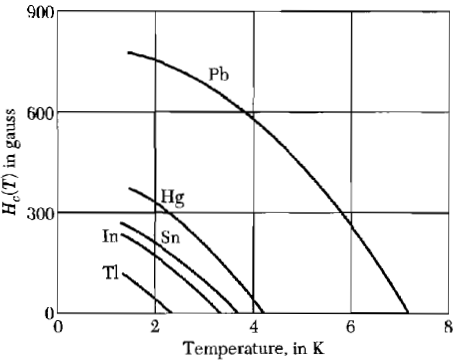
\includegraphics[scale=0.6]{Tcmaterials.PNG}
\caption{"Experimental threshold
curves of the critical field $H_{c}(T)$
versus temperature for several superconductors.
A specimen is superconducting
below the curve and
normal above the curve." \cite{kittel}}
\label{Fig:temp}
\end{figure}

Secondly, a superconductor placed in a weak magnetic
field acts as a perfect diamagnet with zero magnetic induction in the interior,  since the conduction electrons are in a specific order of paired electrons, as  explained by Bardeen, Copper and Schrieffer in 1957. The phenomenon happening inside the superconductor is called Meissner effect, where Meissner and Ochsenfeld observed that the magnetic magnetic field lines are expelled from the sample when it is cooled below $T_{c}$, as illustrated bellow, thus the magnetic field inside the sample is zero along with the magnetic flux.


\begin{figure}[H]
\centering
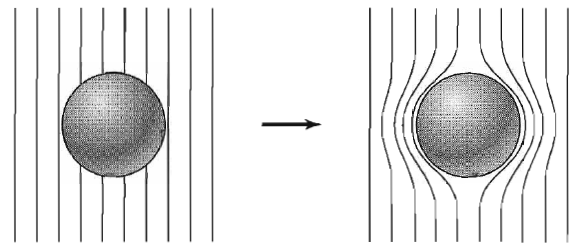
\includegraphics[scale=.5]{Meissner.PNG}
\caption{"Meissner effect in a superconducting sphere cooled in a constant applied magnetic field;
on passing below the transition temperature the lines of induction B are ejected from the sphere."  \cite{kittel}}
\end{figure}

We should mention here that some materials become superconducting only under high pressure, for example Si has a critical temperature at $8.3$ K under $165$ kbar pressure. In this report we will discuss superconductivity  under zero pressure. The resulting $B = 0$ inside the superconductor cannot be derived assuming a medium of zero resistivity, since Ohm's law $\textbf{E} = \rho \textbf{j}$, for $\rho \sim 0$ with $j\sim \infty$ indicates $E=0$, where we obtain $\nabla \times \textbf{E}= -\frac{d \textbf{B}}{dt} =0$ according to Maxwell equation, stating that the flux through the medium cannot change through cooling instead of $B=0$, contradicting Meissner effect, concluding to the fact that perfect diamagnetism is an essential property of the  superconducting state.\\ 



\begin{figure}[H]
\centering
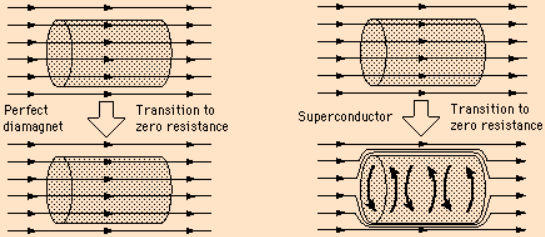
\includegraphics[scale=.9]{diam.PNG}
\caption{\cite{meis}}
\end{figure}




The difference between a superconductor and a perfect
conductor, is that when the latter is placed in a magnetic field cannot produce a permanent eddy current screen, i.e. field penetration. The three factors that come into play are that: below $T_{c}$, the resistivity of the superconductor is zero (Fig \ref{resist} ), above $H_{c}$ the superconductor becomes non-superconducting and the critical current density is the maximum value that a superconductor can carry with zero resistance.\\ 
 
\begin{figure}[H]
\centering
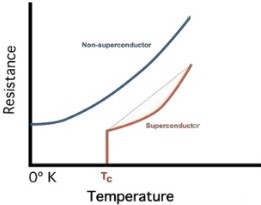
\includegraphics[scale=.9]{Inkedresistancetypes.jpg}
\caption{ \cite{slides}}
\label{resist}
\end{figure}

 
Superconductivity is destroyed by sufficiently strong magnetic field at the critical field value $H_{c}(T)$ which is a function of temperature, as illustrated in Fig \ref{Fig:1}, with $H_{c}(T_{c})=0$.\\

\begin{figure}[H]
\centering
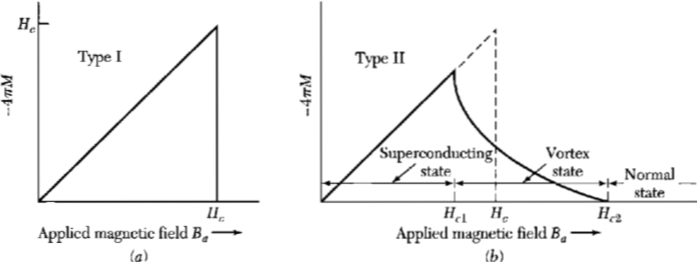
\includegraphics[scale=0.90]{type12.PNG}  
\caption{ Magnetization curves of Type I and II according to the applied magnetic field. \cite{kittel}}
\label{Fig:1}
\end{figure} 
 
 

The magnetization of the superconductor is given by 

\begin{equation}
M = - \dfrac{B_{a}}{4\pi}  \quad (\text{ CGS}) \quad \quad or \quad \quad 
M = - \dfrac{B_{a}}{\mu_{0}}  \quad (\text { SI })
\label{magnetization}
\end{equation}

where $B_{a}$ is the applied magnetic field.\\
 
In Fig \ref{Fig:1}(a) the magnetization curve for a long solid cylinder placed in a longitudinal magnetic field is illustrated, where materials obeying this curve are called Type $I$ superconductors- soft (27 pure metals) because they are characterised by really small $H_{C}$ where the superconducting state disappears suddenly at $T_{C}$. The soft superconductors can tolerate impurities without affecting their superconducting properties and the superconducting current flows only on their surface. \\ Concerning Fig \ref{Fig:1}(b) the materials (alloys or transition metals with short electronic mean free path in the normal state) are referred to as Type $II$ superconductors-hard maintaining a superconducting phase upto higher critical field $H_{c2}$ and critical temperature. For the latter, the flux density is non zero and the Meissner effect is incomplete at the Vortex state where the superconductor is threaded with flux lines, i.e. in the phase between the lower $H_{c1}$ and the upper critical field $H_{c2}$, with the latter being usually 100 times bigger than $H_{c}$. The hard superconductors cannot tolerate impurities without affecting their superconducting properties and the current is found to flow throughout their material. In this experiment we used a Type $I$ superconductor, so we will restrain to its description.\\


 






\section{Magnetization of a superconductor}

Magnetic susceptibility $\chi$ is the degree of Magnetization of a material $M$, in response to an applied magnetic field intensity $H$, given by

\begin{equation}
M = \chi H
\end{equation}

\begin{equation}
B= \mu_{0}(1+\chi) M
\end{equation}


The superconducting materials have very large and negative susceptibility $\chi=-1$. The temperature dependence of their magnetization exists only under the critical temperature as described  through the Meissner effect.
Referring to diamagnetic atoms, that are non-magnetic atoms, the valence electron rotating the nucleus induces a magnetic moment, but due to the different orientations of the atomic orbits their net magnetic moment is zero. When a magnetic field $H$ is applied, the induced magnetic moment is in the opposite direction of the applied field

\begin{equation}
M=-H
\end{equation}

As described through the Meissner effect, superconductivity is a quantum state of matter with zero electrical resistance and magnetic field expulsion below $T_{c}$. If we approach a superconductor with a magnet, the change of the magnetic flux $\dfrac{d\Phi}{dt}$ must be zero, since we started without a magnetic flux. Thus the superconductor induces a magnetic field that repels that of the magnet (principle of quantum levitation) implying the magnetic susceptibility $\chi=-1$ (SI).\

The magnetic permeability of the free space, as well as of the Normal phase in a superconductors, is by definition 

\begin{equation}
\mu \equiv \frac{B}{H}=1
\end{equation}

In a cylindrical specimen in the Meissner state, due
to continuity of the tangential component of H, inside it we have $B=0$ and $H_{i}=H$.



\subsubsection{Demagnetizing factor}
When the applied magnetic field is near the critical value, the shape of the sample becomes important because depending on its geometry the field lines are not equally dense around the sample's surface thus the magnetic field is increased locally over some areas, as illustrated in Fig \ref{diamshap}.
The demagnetizing factor $\eta$ is well defined for ellipsoidal shapes through the relation 
\begin{equation}
1- \eta < \dfrac{H}{H_{C}} <1
\end{equation}


\begin{figure}[hbtp]
\centering
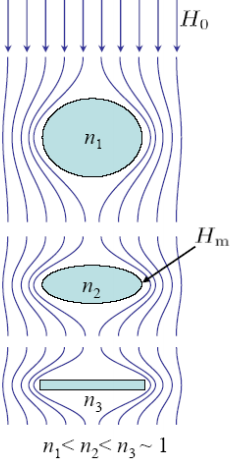
\includegraphics[scale=.8]{demagsha.PNG}
\caption{Demagnetizing factor of typical shapes. $H_{0}$ corresponds to the apllied magnetic field $H$ and $H_{m}$ to the critical field referenced to the surface $H_{C}$, according to our notation. \cite{demag}}
\label{diamshap}
\end{figure}



Specifically, for a long thin cylinder or a thin plate parallel to the field is zero, $1/3$ for a sphere and $1/2$  for a cylinder in a transverse field. An infinite flat slab placed in a perpendicular field has a factor of one.\\

The demagnetizing field of an ellipsoid is uniform and parallel to the applied external field thus $H_{d}=-\chi DM$ and $H_{i}=\chi M$, allowing us to derive the formula for $\eta$, that will be named D from now on, considering the magnetic field inside the sample

\begin{equation}
M=\chi H_{i} =\chi H_{a}- \chi D M
\end{equation}

giving  


\begin{equation}
M= \dfrac{\chi}{1+\chi D} H_{a}
\end{equation}

Naming $H_{m}$ the field corresponding to $-Mmax$ for $H<H_{C}$, according to 
Fig \ref{magtan}

\begin{figure}[H]
\centering
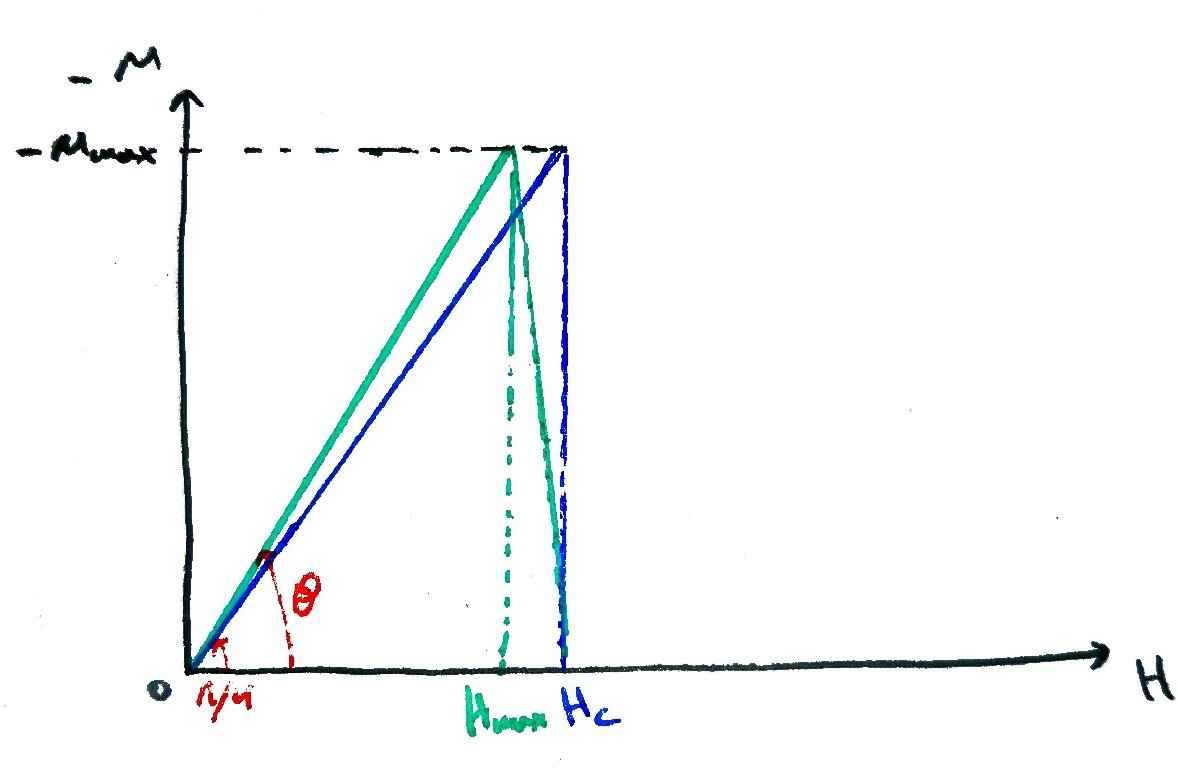
\includegraphics[scale=.5]{magtan.jpg}
\caption{\label{magtan}}
\end{figure}


\begin{equation}
tan\dfrac{\pi}{4}=1=-\dfrac{M_{max}}{H_{C}}
\end{equation}

and

\begin{equation}
tan \theta =-\dfrac{M_{max}}{H_{m}}=\dfrac{1}{1-D}
\end{equation}


where substituting $-M_{max}=H_{C}$
we obtain 



\begin{equation}
D= 1- \dfrac{H_{max}}{H_{C}}
\label{D}
\end{equation}


As it will be explained in the next section, the areas  included in the two curves should be the same, once they correspond to the free Gibbs energy.






\subsubsection{London Equation}


First, Ohm's law was modified to obtain the Meisnner effect describing the conduction in the superconducting state.  London equation was derived assuming that the current density in the superconducting state is directly proportional to the vector potential $\textbf{A}$ of the magnetic field where $\textbf{B}= \nabla \times \textbf{A}$.
The London equation is given in two forms as
\begin{equation}
 \textbf{j}=-\frac{1}{\mu_{0} \lambda_{L}^{2}} \mathbf{A}
\quad or \quad
  \nabla \times \mathbf{j}=-\frac{1}{\mu_{0} \lambda_{L}^{2}} \mathbf{B} \quad (\text { SI })
\end{equation}

where the first one
applies to a simply connected superconductor, where additional terms may be present in a ring or cylinder, and the second form holds true independent of geometry. Here $\lambda_{L}$ is a constant with the dimensions of length.\\

Using Maxwell equation under static conditions
\begin{equation}
\nabla \times \textbf{B}=\mu_{0} \textbf{j}
\end{equation}

curling both sides

\begin{equation}
\text { curl curl } \mathbf{B}=-\nabla^{2} \mathbf{B}=\mu_{0} \nabla \times \mathbf{j}
\end{equation}

we combine it with London equation to obtain

\begin{equation}
\nabla^{2} \mathbf{B}=\mathbf{B} / \lambda_{L}^{2}
\label{Meissnereq}
\end{equation}


The above equation (\ref{Meissnereq}) represents the Meissner effect, since it does not have a solution uniform in space, so a uniform magnetic field cannot
exist in a superconductor, i.e. the only acceptable solution is $\textbf{B}(\textbf{r})=const=0$, ensuring that $\textbf{j}=0$ always (for $B=0$). 


\begin{figure}[H]
\centering
\caption{\cite{kittel}}
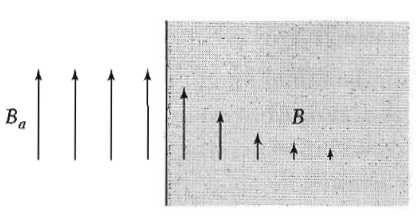
\includegraphics[scale=0.7]{penetration.PNG}    
\label{Fig:pen}
\end{figure}

As illustrated above in Fig \ref{Fig:pen}, in the pure superconducting state the only field allowed is exponentially
damped as we go in from an external surface.

Inside a semi-infinite superconductor, the field is given by
\begin{equation}
B(x)=B(0) \exp \left(-x / \lambda_{L}\right)
\label{penetr}
\end{equation}
where $B(0)$ is the field at the boundary of the plane and $\lambda_{L}$ now is the London penetration depth giving the depth of the magnetic field, characterizing
a superconductor 

\begin{equation}
\lambda_{L}=\left(\epsilon_{0} m c^{2} / n q^{2}\right)^{1 / 2} \quad (SI)
\end{equation}

with $q$ the particle charge, $m$ the mass and $n$ the concentration.\\

An applied magnetic field B, will penetrate a thin film fairly uniformly if
the thickness is much less than $\lambda_{L}$; thus in a thin film the Meissner effect is not
complete. In a thin film the induced field is much less than $B_{a}$ and there is
little effect of $B_{a}$, on the energy density of the superconducting state, so that
(6) does not apply. follows that the critical field H, of thin films in parallel
magnetic fields will be very high.

\subsubsection{Coherence Length}
The coherence length  $\xi_{0}$ is a measure of the distance within which the superconducting electron concentration cannot change drastically in a spatially varying magnetic field and is a measure of the range over
which we should average \textbf{A} to obtain \textbf{j}.


Coherence length is described by the Landau-Ginzburg equations and depends on the Fermi velocity and the energy gap of a superconductor, supporting the fact that the electron density of a superconductor cannot change rapidly. The intrinsic coherence length is given by
\begin{equation}
\xi_{0}=-\frac{2 \hbar v_{F}}{\pi E_{g}}
\end{equation} 

where, $V_{F}$is the Fermi velocity and $E_{g}$ is the superconducting band gap. The coherence length provides a criterion for the purity of the superconductor, the bigger the purer, for each material.
 
\subsubsection{Intermediate state}

"Intermediate state is defined as a thermodynamically equilibrium state in which a type-I
superconductor is split for domains of superconducting and normal phases " \cite{intermediate}.


Concerning to a field strong enough to ruin superconductivity, we have to consider the effect of the demagnetizing factor (when $\neq0$) because everywhere along the surface of a thin layer comparing to $\lambda _{L}$, $B\neq0$. Within the sample according to Eq (\ref{penetr}), B will penetrate in the sample according to its geometry for $H_{i}<H<H_{C}$, leading to the so called intermediate state.

\begin{figure}[H]
\centering
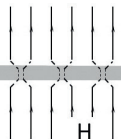
\includegraphics[scale=1]{flatslab.PNG}
\caption{Cross-sectional view of an infinite slab ($D=1$) in a weak magnetic field H, in the intermediate state starting from any H exceeding zero. \cite{intermediate}}
\end{figure}

Inside a uniform ellipsoid when H is parallel to its axis, $H_{i}= \frac{H}{1- D}$, thus near the poles the field will be zero and near the equator $H_{C}=2H$, so when H is increased beyond this value superconductivity will be destroyed, but not completely because there is still left a lot of condensation energy in the specimen. \cite{intermediate} Concluding, the outer thin layer of the ellipsoid will be in the normal state and the inner superconducting. In reality an inhomogeneous superconductor has different  critical temperatures along its bulk, usually $T_{C1}<T<T_{C2}$ with $T_{C1}$ and  $T_{C2}$ random, so the intermediate state consists of regions of normal and superconducting material, as illustrated in Fig \ref{intermediate}.


\begin{figure}[hbtp]
\centering
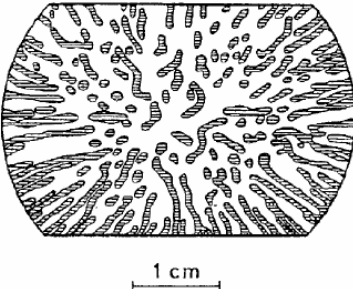
\includegraphics[scale=.61]{intermediate.PNG}
\caption{Distribution of superconducting and normal regions in a tin sphere. \cite{demag}}
\label{intermediate}
\end{figure}
 
 
 \subsubsection{ Meissner fraction}

 The magnetization of a sample including its volume factor is $M=-\frac{B}{V \mu}$, where we obtain the superconducting volume fraction called Meissner fraction, as the magnetization of the whole sample will be given by $M=-\dfrac{V_{S}}{V_{N}} \dfrac{B_{a}}{\mu}$ obtaining $- \chi =- \dfrac{M}{H}=\dfrac{V_{S}}{V_{N}} <1$
 


\subsection{Thermodynamical approach of superconductivity}


Thermodynamics provided a theoretical understanding of the phenomena associated with supercondnctivity, where many results are described by the phenomenological
equations of London and Landau-Ginzburg, because the transition between the normal and superconducting states is thermodynamically
reversible, thus we can obtain an expression for the entropy difference between the
normal and superconducting states in terms of the critical field curve $H_{c}$ versus T.


In a type $I$ superconductor with a complete Meissner effect ($B=0$ inside the superconductor) $H_{c}$ is a quantitative
measure of the free energy difference between the superconducting and
normal states at constant temperature, which can be determined by calorimetric or magnetic measurements.
In the latter method the stabilization free energy is found from the
value of the applied magnetic field that will destroy the superconducting
state at constant temperature. 
The work done on a superconductor when it is brought reversibly at constant temperature from a position at infinity (where the applied field is zero) to a position
$\textbf{r}$ in the field of a permanent magnet per unit volume of specimen

\begin{equation}
W= -\int _{0}^{Ba} \textbf{M} \cdot d \textbf{B}_{a}
\end{equation}

appears in the magnetic field energy as

\begin{equation*}
dF= - \textbf{M} \cdot d\textbf{B}_{a} =  -\dfrac{ B_{a} dB_{a}}{\mu_{0}} \quad (SI)
\end{equation*}
according to Eq \ref{magnetization}, thus the increase of the Free energy density of the superconductor being brought from a position where the applied field is zero to a position
where the applied field is $B_{a}$, is given by 
\begin{equation}
\Delta F_{s} =F_{s}(B_{a})-F_{s}(0)= \dfrac{B_{a}^{2}}{2\mu_{0}} \quad (SI)
\end{equation}



\begin{figure}[H]
\centering
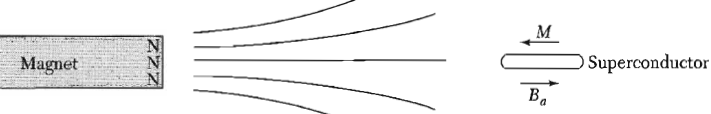
\includegraphics[scale=0.6]{work.PNG}
\caption{Complete Meissner effect in a Type $I$ superconductor. \cite{kittel}}
\label{work}
\end{figure}

We should stress here that $H_{c}=B_{a,c}/ \mu_{0} $ in (SI) and $H_{c}=B_{a,c}$ in (CGS).\\

Now considering a normal nonmagnetic metal, neglecting the small
susceptibility in the normal state, $M = 0$ thus its energy is independent of the applied magnetic field, so 

\begin{equation}
F_{N}(B_{a,c)}=F_{N}(0)
\label{normal}
\end{equation}

Combining Eq \ref{work} and \ref{normal}, including that at $B_{a,c}$ the energies are equal in the normal and superconducting
states, we obtain

\begin{equation}
F_{N}(B_{a,c})= F_{S}(B_{a,c})= F_{S}(0) + \dfrac{B_{a}^{2}}{2 \mu_{0}} \quad (SI)
\label{freeE}
\end{equation}



 
The critical field $H_{C}$ is associated with the energy per volume required to hold out the applied magnetic field, empirically found that is approximated by the parabolic law as \cite{tinkham}

 
 \begin{equation}
H_{C}\simeq H_{C0} [1- (\dfrac{T}{T_{C}})^{2}]
\label{HC}
\end{equation}
 
 
 \begin{figure}[H]
\centering
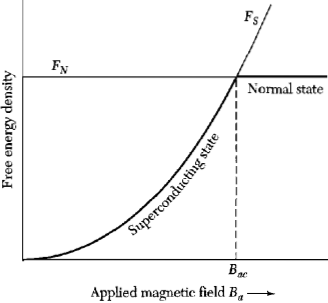
\includegraphics[scale=.7]{freeEn.PNG}
\caption{The free energy density F occurring in the normal and superconducting state. \cite{kittel}}
\end{figure} 
 
 
 
 
 
\subsection{BCS theory of Superconductivity} 
 
The quantum theory of superconductivity was given by Bardeen, Cooper, and Schrieffer in 1957, providing the basis to Josephson and Anderson who discovered the importance of the phase of the superconducting wavefunction. The disappearance of electrical resistivity in the superconductors was modelled in terms of electron pairing in the crystal lattice, called BCS theory. \cite{1},\cite{kittel}\  
BCS theory explains the attractive interaction between electrons responsible for the electron pairing leading to a ground state separated from the excited states by an energy gap, and how the latter affects the thermal and electromagnetic properties, including $T_{C}$. The so called indirect electron-lattice-electron interaction is observed when an electron sees the deformation of another electron interaction with the lattice and adjusts itself to take advantage of the deformation to lower its energy interacting with the first electron, responsible finally for the energy gap in the superconductors on the order of $0.001$ eV which inhibits the kind of collision interactions leading to ordinary resistivity, thus for temperatures corresponding to thermal energy less than the band gap, the material exhibits zero resistivity. The coupling to the lattice is called phonon interaction and the energy gap is related to the coherence length. Furthermore, the BCS theory supports the penetration depth and the coherence length because the Meissner effect is obtained naturally once the London equation is obtained for slowly varying magnetic fields. The criterion for the transition temperature is provided by the electrical
resistivity at room temperature, once it is a measure of the electron-phonon interaction, where the higher the resistivity at room temperature the more likely it is that the metal will be a superconductor when it gets cooled. The best conductors at room temperature (gold, silver, and copper) do not become superconducting at all because they have the smallest lattice vibrations, so their behavior correlates well with the BCS Theory. On the other hand, the superconductors are really poor conductors. Finally the  quantization of the magnetic flux in the superconducting ring is quantized and the macroscopically occupied single quantum state - condensate flowing without resistanve known as the BCS ground state occuring below $T_{C}$ consists of pairs of electrons close to the Fermi level, the so called Cooper pairs, where the one-particle orbitals are filled in pairs behaving like bosons with zero spin; if a particle with wavevector and spin $k\uparrow$ is occupied then the particle with wavevector $k\downarrow$ is also occupied.  \cite{kittel} 



\subsubsection{Superconducting ring} 

The flux quantization mentioned above is a long-range quantum effect in which
the coherence of the superconducting state extends over a ring.
The energy density of an electric field containing a large number of photons is given by
\begin{equation}
E^{*}(\mathbf{r}) E(\mathbf{r}) / 4 \pi \cong n(\mathbf{r}) \hbar \omega
\end{equation}

where $E(\textbf{r})$ is the electric field intensity and $n(\textbf{r})$ the number density of photons. Using the semi-classical approximation we obtain a probability amplitude that describes the Cooper pairs
\begin{equation}
E(\mathbf{r}) \cong(4 \pi \hbar \omega)^{1 / 2} n(\mathbf{r})^{1 / 2} e^{i\theta r} 
\end{equation}

with $\theta(r)$ the phase of the field.\
Assuming a boson gas with a large number of bosons in the same orbital, the amplitude and phase are significant quantities. The quantization of the magnetic flux is a result of proving that a boson gas obeys the London equation.\
Supposing that the pair concentration $n=\psi^{*} \psi$ is constant, at absolute zero it will be equal to half of the concentration of the electrons in the conduction band, giving a pair probability amplitude 

\begin{equation}
\psi=n^{1 / 2} e^{i \theta(r)}  \quad \psi^{*}=n^{1 / 2} e^{-i \theta(r)}
\end{equation}

The pair velocity is given by

\begin{equation}
\mathbf{v}=\frac{1}{m}\left(-i \hbar \nabla-\frac{q}{c} \mathbf{A}\right)
\end{equation}

and the flux by

\begin{equation}
\psi^{*} \mathbf{v} \psi=\frac{n}{m}\left(\hbar \nabla \theta-\frac{q}{c} \mathbf{A}\right)
\end{equation}

thus the electric current density is

\begin{equation}
\mathbf{j}-q \psi^{*} \mathbf{v} \psi=\frac{n q}{m}\left(\hbar \nabla \theta-\frac{q}{c} \mathbf{A}\right)
\label{current}
\end{equation}


where taking the curl on both sides we obtain the London equation
\begin{equation}
\nabla \times \mathbf{j}=-\frac{n q^{2}}{m c} \mathbf{B}
\end{equation}

Taking a closed path on the inside of a superconducting ring away from its surface, as illustrated in Fig \ref{Fig:ring}, the Meissner effect imposes $\textbf{B}$ and $\textbf{j}$ to be zero, so according to Eq \ref{current} we obtain 

\begin{equation}
\hbar c \nabla \theta = q\textbf{A}
\end{equation}


The phase change completing a full circle once gives $\theta_{2}-\theta_{1}=2 \pi s$, with $s$ an integer number.

\begin{figure}[H]
\centering
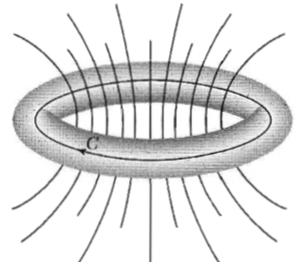
\includegraphics[scale=0.60]{ring.png}   
\caption{Flux lines emurcing from the superconducting currents flowing on the surface of the supoerconducting ring. \cite{kittel}}
\label{Fig:ring}
\end{figure}
 


Using Stoke's theorem $
\oint_{C} \mathbf{A} \cdot d l=\int_{C}(\nabla \times \mathbf{A}) \cdot d \sigma=\int_{C} \mathbf{B} \cdot d \sigma=\Phi$, with $d\sigma$ the area, we finally obtain the quantized magnetic flux $\Phi$ through the ring contour $C$ by
\begin{equation}
\Phi=(2 \pi \hbar c / q) s
\end{equation}

For a cooper pair the appropriate 'particle' charge is $q=-2e$ and by substituting $s=1$, we obtain the fluxation quanta called fluxoid $\Phi_{0}=2 \pi \hbar / 2e  $.














\chapter{Experimental Setup}

The main part of the apparatus are the coils producing and measuring the magnetic fields. Specifically, the primary coil (1)\ref{setup} produces the magnetic external field and the astatic pair of identical coils (3)\ref{setup} measures the sample's magnetic moment. To obtain the magnetization of the sample, a superconducting flux transformer transfers the magnetic flux to a flux-gate magnetometer \ref{fluxmag}, where its probe is located in the magnetometer coil which is part of the flux
transformer. The flux heater (6)\ref{setup} 
is in thermal contact to a part of the flux transformer circuit, used to heat a part
of the wire to its normal state to remove any super current flowing in the circuit. The sample heater (4)\ref{setup} heats up the sample, who's temperature is measured by a resistor (5)\ref{setup} with a given calibration curve.

\begin{figure}[H]
\centering
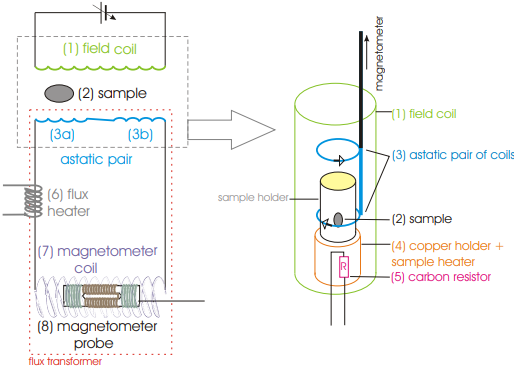
\includegraphics[scale=1.15]{experiment.PNG}   
\caption{ Experimental assembly and coil positions. \cite{script}}
\label{setup}
\end{figure}

\begin{figure}[H]
\centering
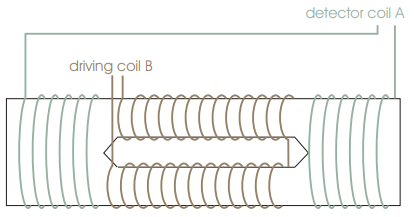
\includegraphics[scale=0.90]{Magnetometerprobe.PNG}    
\caption{Probe of the flux gate magnetometer.\cite{script}}
\label{fluxmag}
\end{figure}


Coil (3a) measures both the
primary field and the induction due to the magnetized sample, while (3b) only the primary field having the same value as at the sample position. Their  windings are opposite in
order to counterbalance the signal produced by the primary field, but the compensation is not exact, so a signal proportional to the primary field survives which appearing as a linear background in the field dependent measurements.


\begin{figure}[hbtp]
\centering
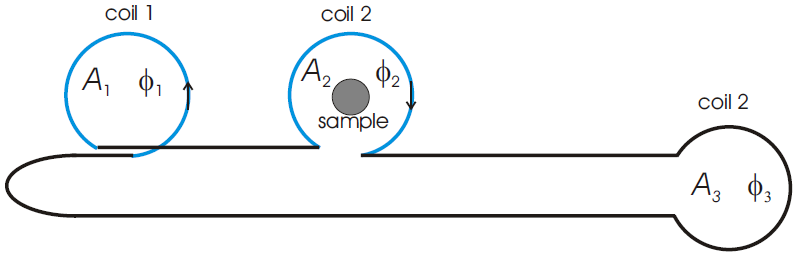
\includegraphics[scale=0.6]{fluxtrans.PNG}
\caption{flux transformer}
\end{figure}



The flux transformer is based on the principle that the magnetic flux around the area surrounding the superconductor does not change. The total flux is given by
\begin{equation}
\begin{array}{c}{\Phi _{tot}= A_{1} \Phi_{1} +A_{2} \Phi _{2} + A_{3} \Phi _{3}= const
}\end{array}
\end{equation}

with $\Phi _{1}= \mu H$, $\Phi_{2}=\mu (H+M)$ and $\Phi _{3}$ measured, assuming $A_{1}=A_{2}$.

The blue coils $1$ and $2$ are the astatic pair and coil $3$ the magnetometer coil.\\

Measuring a change in $H$ and ${\Phi} _{3}$ we can calculate the change in $M$.\\

Considering the change through the two areas

\begin{equation}
         \begin{array}{c}{   0 =\Delta \Phi_{1}+\Delta \Phi_{2}=A_{1} N_{1} \Delta B_{1}+A_{2} N_{2} \Delta B_{2}} \\  \\ {\Delta B_{2}=-\frac{A_{1} N_{1}}{A_{2} N_{2}} \Delta B_{1}}\end{array}
\end{equation}

with A the area of the superconducting circuit and N the number of windings of the coil.\\

The coil system is contained in a bath of liquid He at $4.2K$. Moreover, the sample heater is coiled on the copper holder where the sample is placed. \\
 It consists of a ferrite core which is wounded by a driving coil and the detector coil. The coil goes through hysteresis because of the alternating current since the permeabily $\mu$ of a ferromagnet depends on the field. As a result, an electrical current is produced in the second coil which is then measured by a detector. When an external constant field $H_{G1}$ is applied, it changes the hysteresis curve. The core is more easily aligned in the direction of the field. As a consequence, output current and the alternating magnetic field will not be in phase with the input current.\\
In this experiment, the driving coil does not pay any role in the output signal since the magnetic flux remains within the ferrite core. The flux $\Phi=\mu(H(t)) \mu_{0} H_{G 1} A$ generated by the constant field $H_{G1}$ is measured by the detector. Therefore, the current changes with the constant field. 


















\chapter{Analysis}

We performed the two main tasks of this experiment: Firstly the Magnetization Curves were obtained for twelve different temperatures, secondly the Meissner-Ochsenfeld effect was observed from the magnetization curves of ten different field strengths.



 
 
\section{Magnetization curves characterized by temperature} 
To obtain the magnetization curves, we increased the heater current from $0.025 \rightarrow 0.365 A$ in steps of approximately $0.025A$ to acquire the full range of the temperature of interest, setting a swiping rate of $0.2 A/min$ and then recorded the voltage against the coil current $(0 \rightarrow 1A)$. For each plot we used the equation \begin{equation}
T=1.017+6.07 * \exp (-R / 1700)+40.6 * \exp (-R / 170)  \quad
 K
\end{equation}

provided from the script to convert the resistance given from the heater current to temperature.\\

Our task was to subtract the linear background signal, fitting it in the high field region using the OriginLab program, in order to determine the $H_{C}$ values and plot them as a function of temperature using the fitting equation \ref{HC}.


Bellow, the magnetization curves are illustrated starting from the lowest temperature. We excluded from our analysis the curve corresponding to $4.26 K$ measurement because a proper background subtraction was not possible due to the anomaly in the beginning of the data acquisition, where something that we are not aware of, went wrong in the lab equipment for a second resulting to this. Also the plot corresponding to $7.17 K$ was excluded because it contains only background noise. 




 

\begin{figure}[H]
\begin{center}
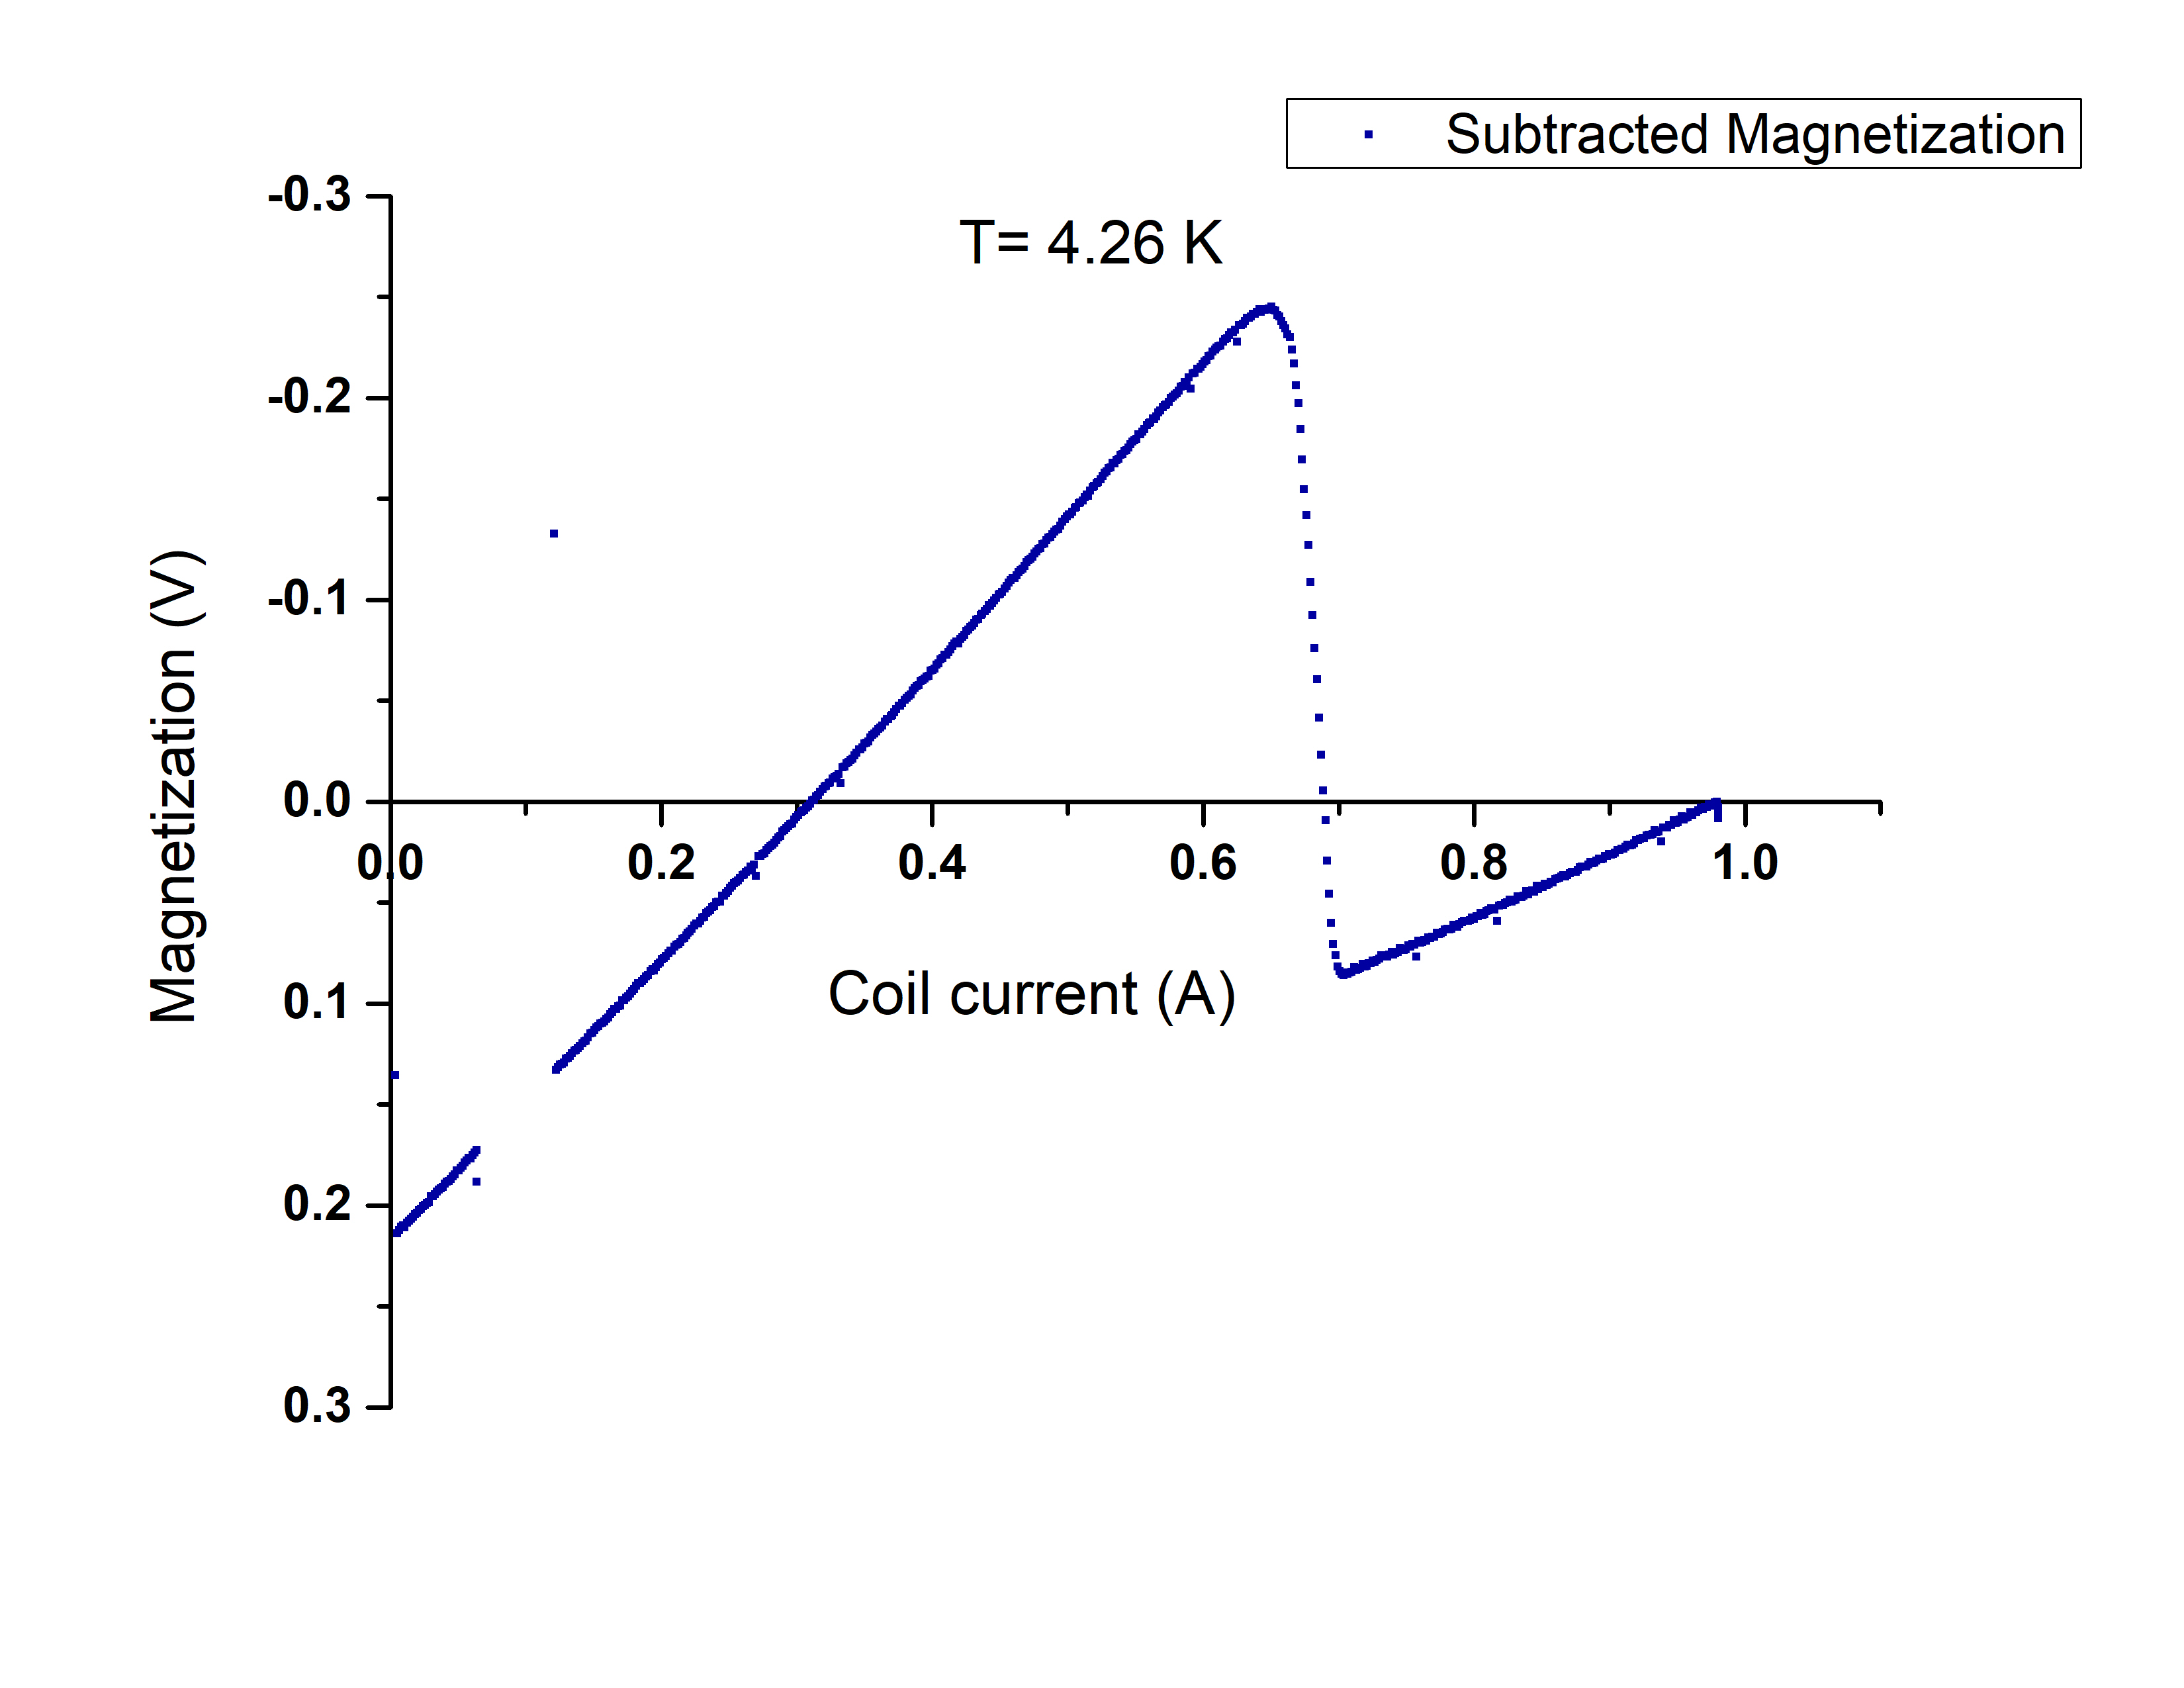
\includegraphics[scale=0.5]{426.jpg}
\end{center}
\end{figure}



\begin{figure}[H]
\begin{center}
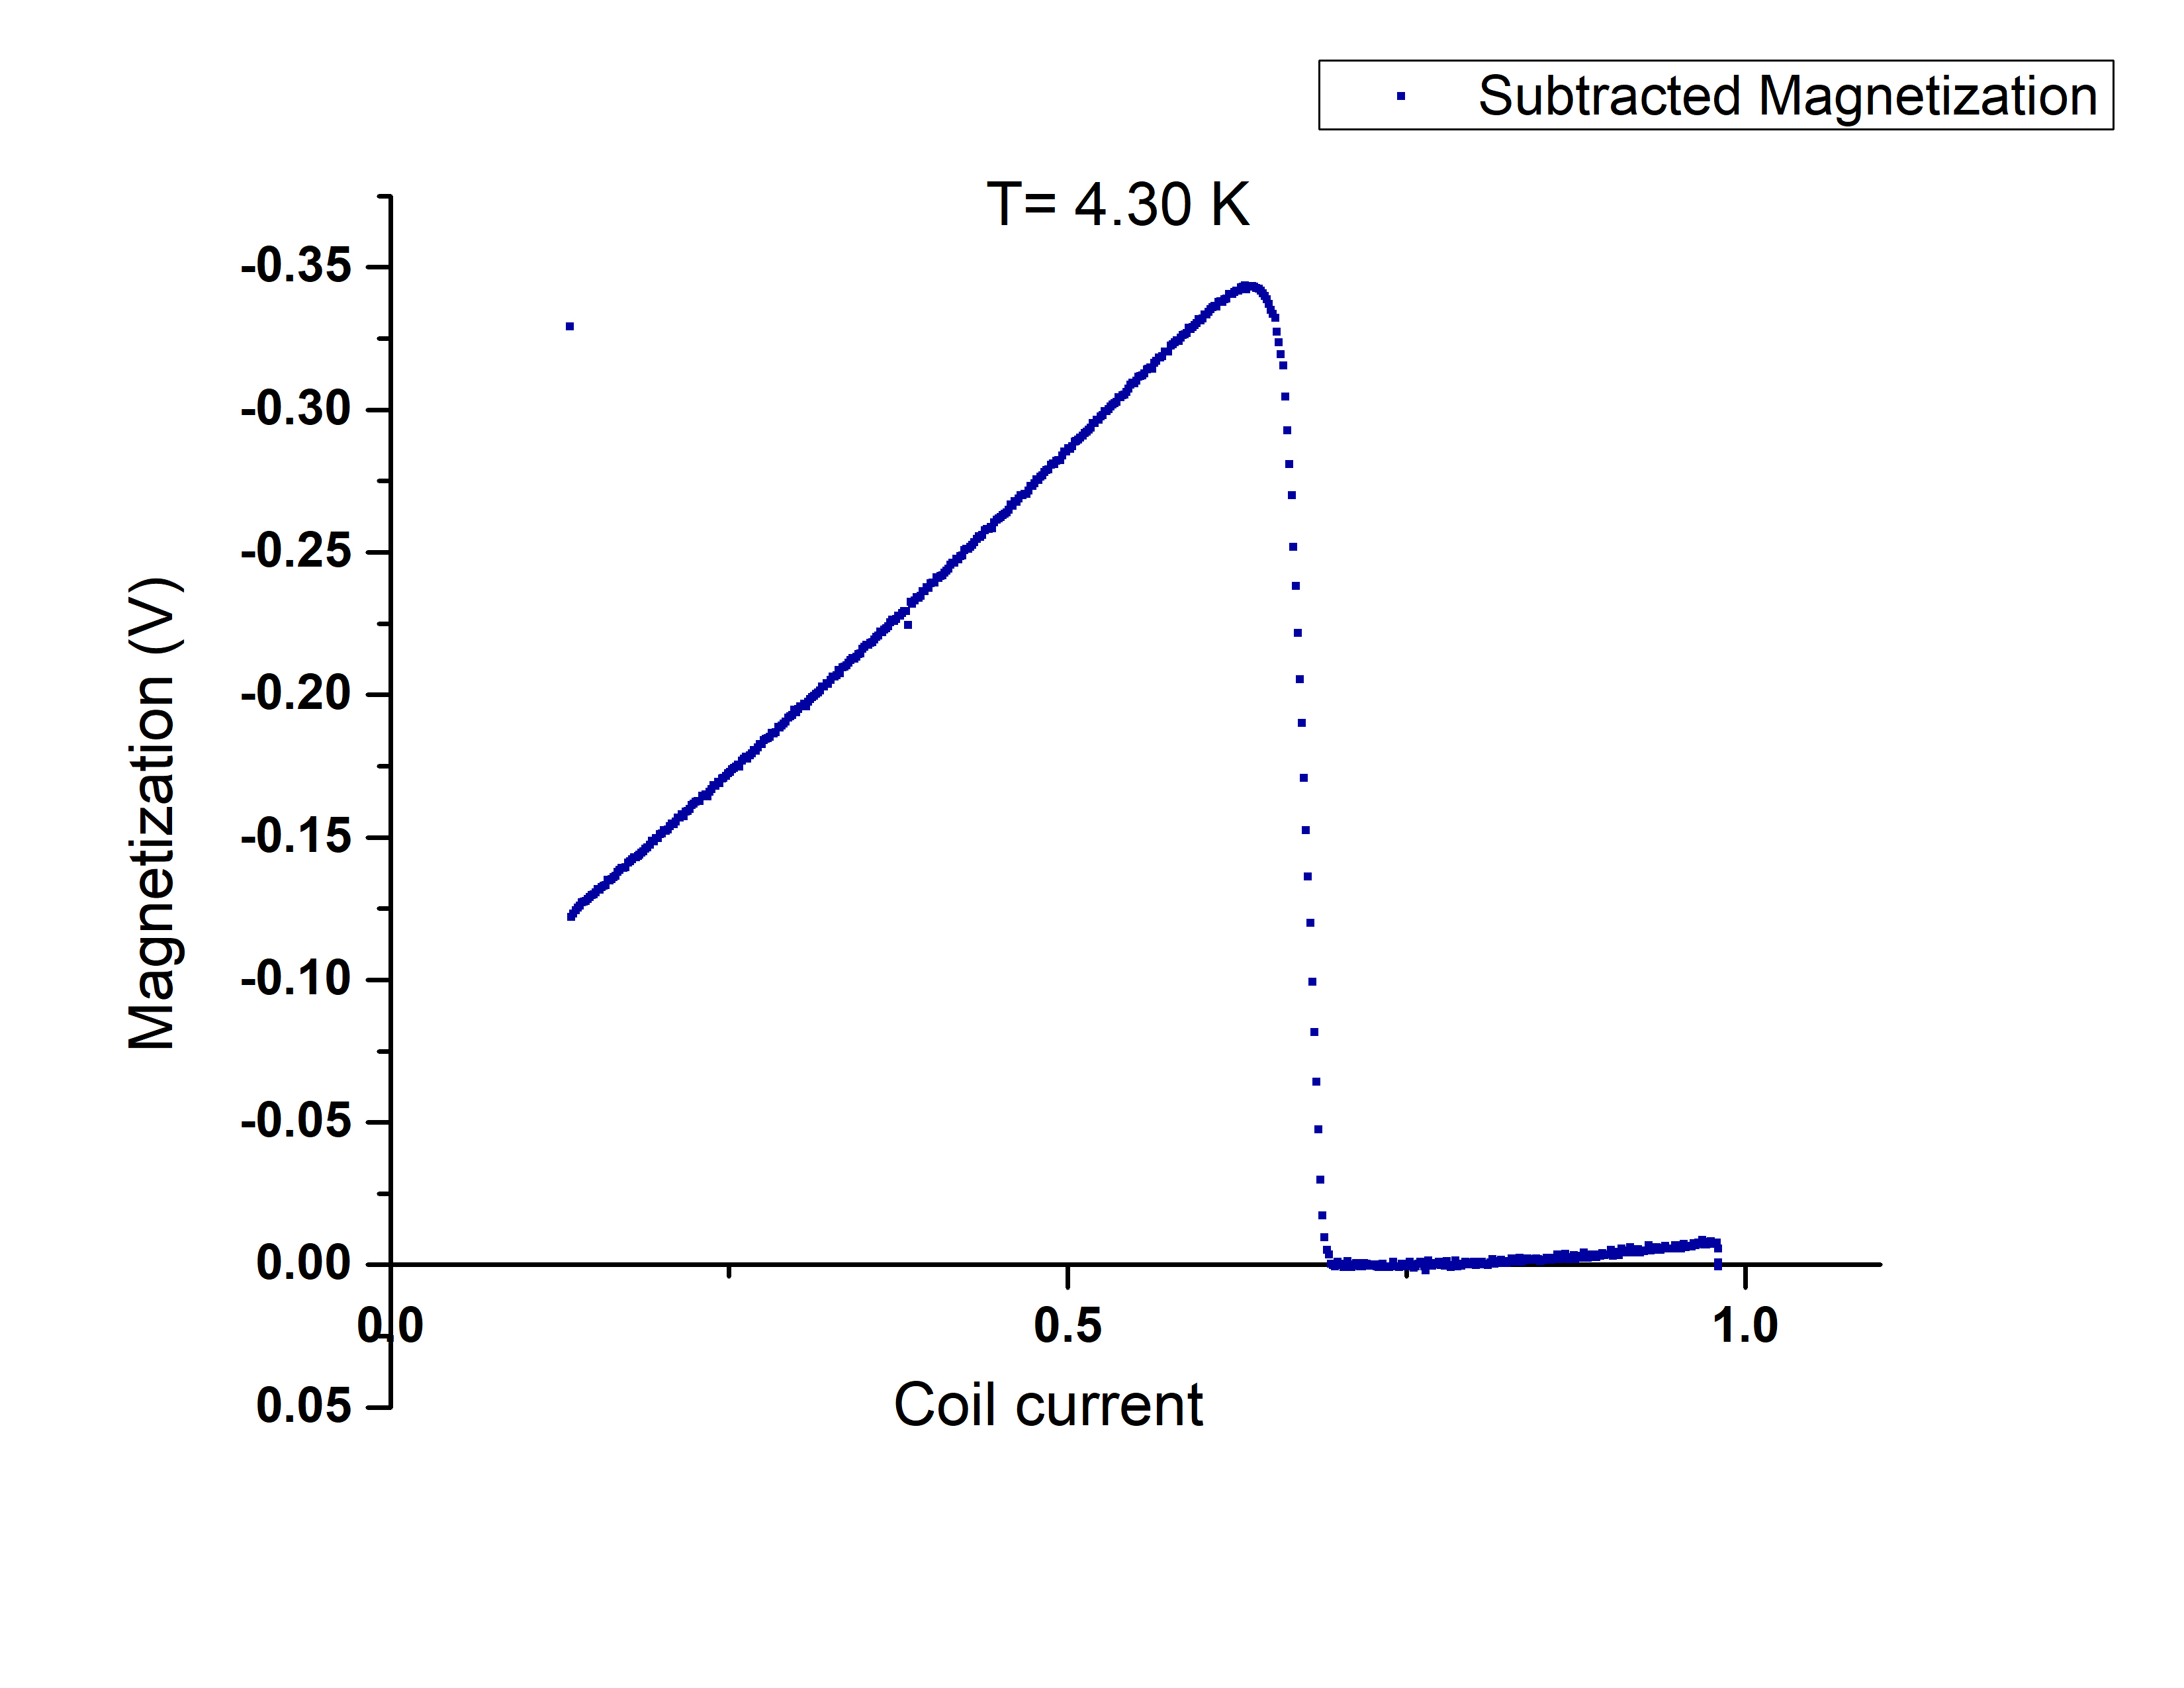
\includegraphics[scale=0.5]{430.jpg}
\end{center}
\end{figure}



\begin{figure}[H]
\begin{center}
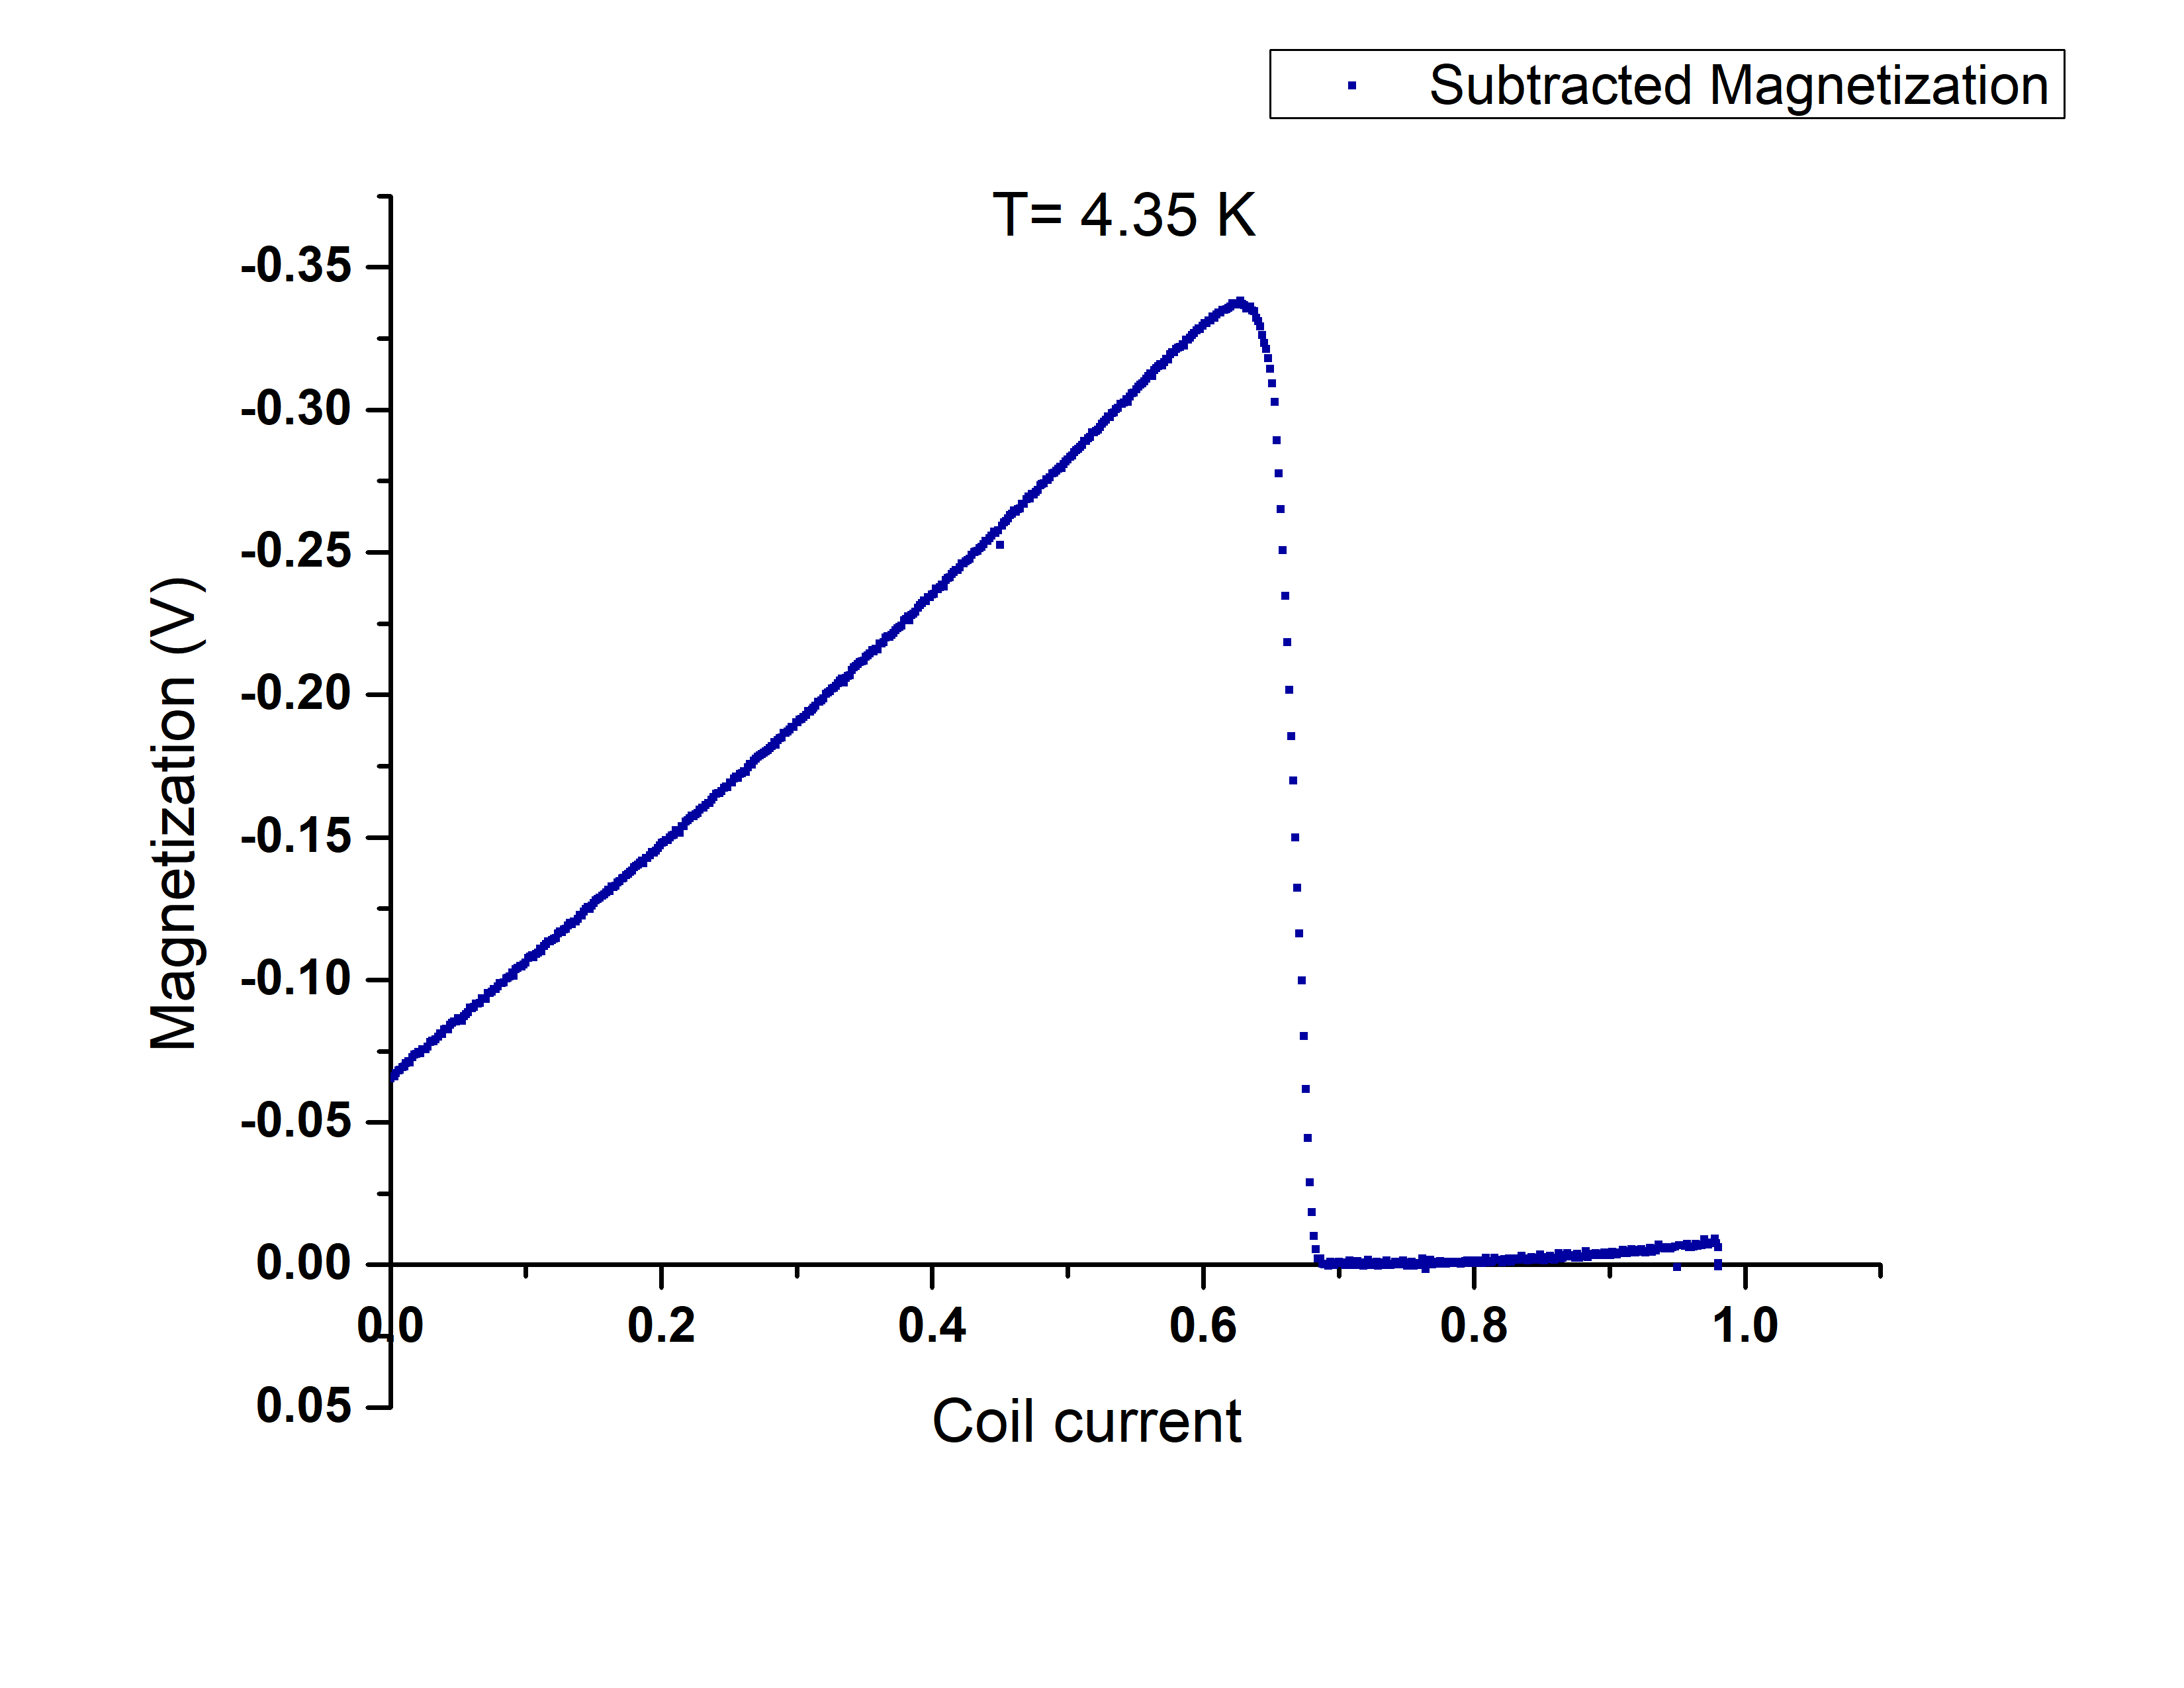
\includegraphics[scale=0.5]{435.jpg}
\end{center}
\end{figure}


\begin{figure}[H]
\begin{center}
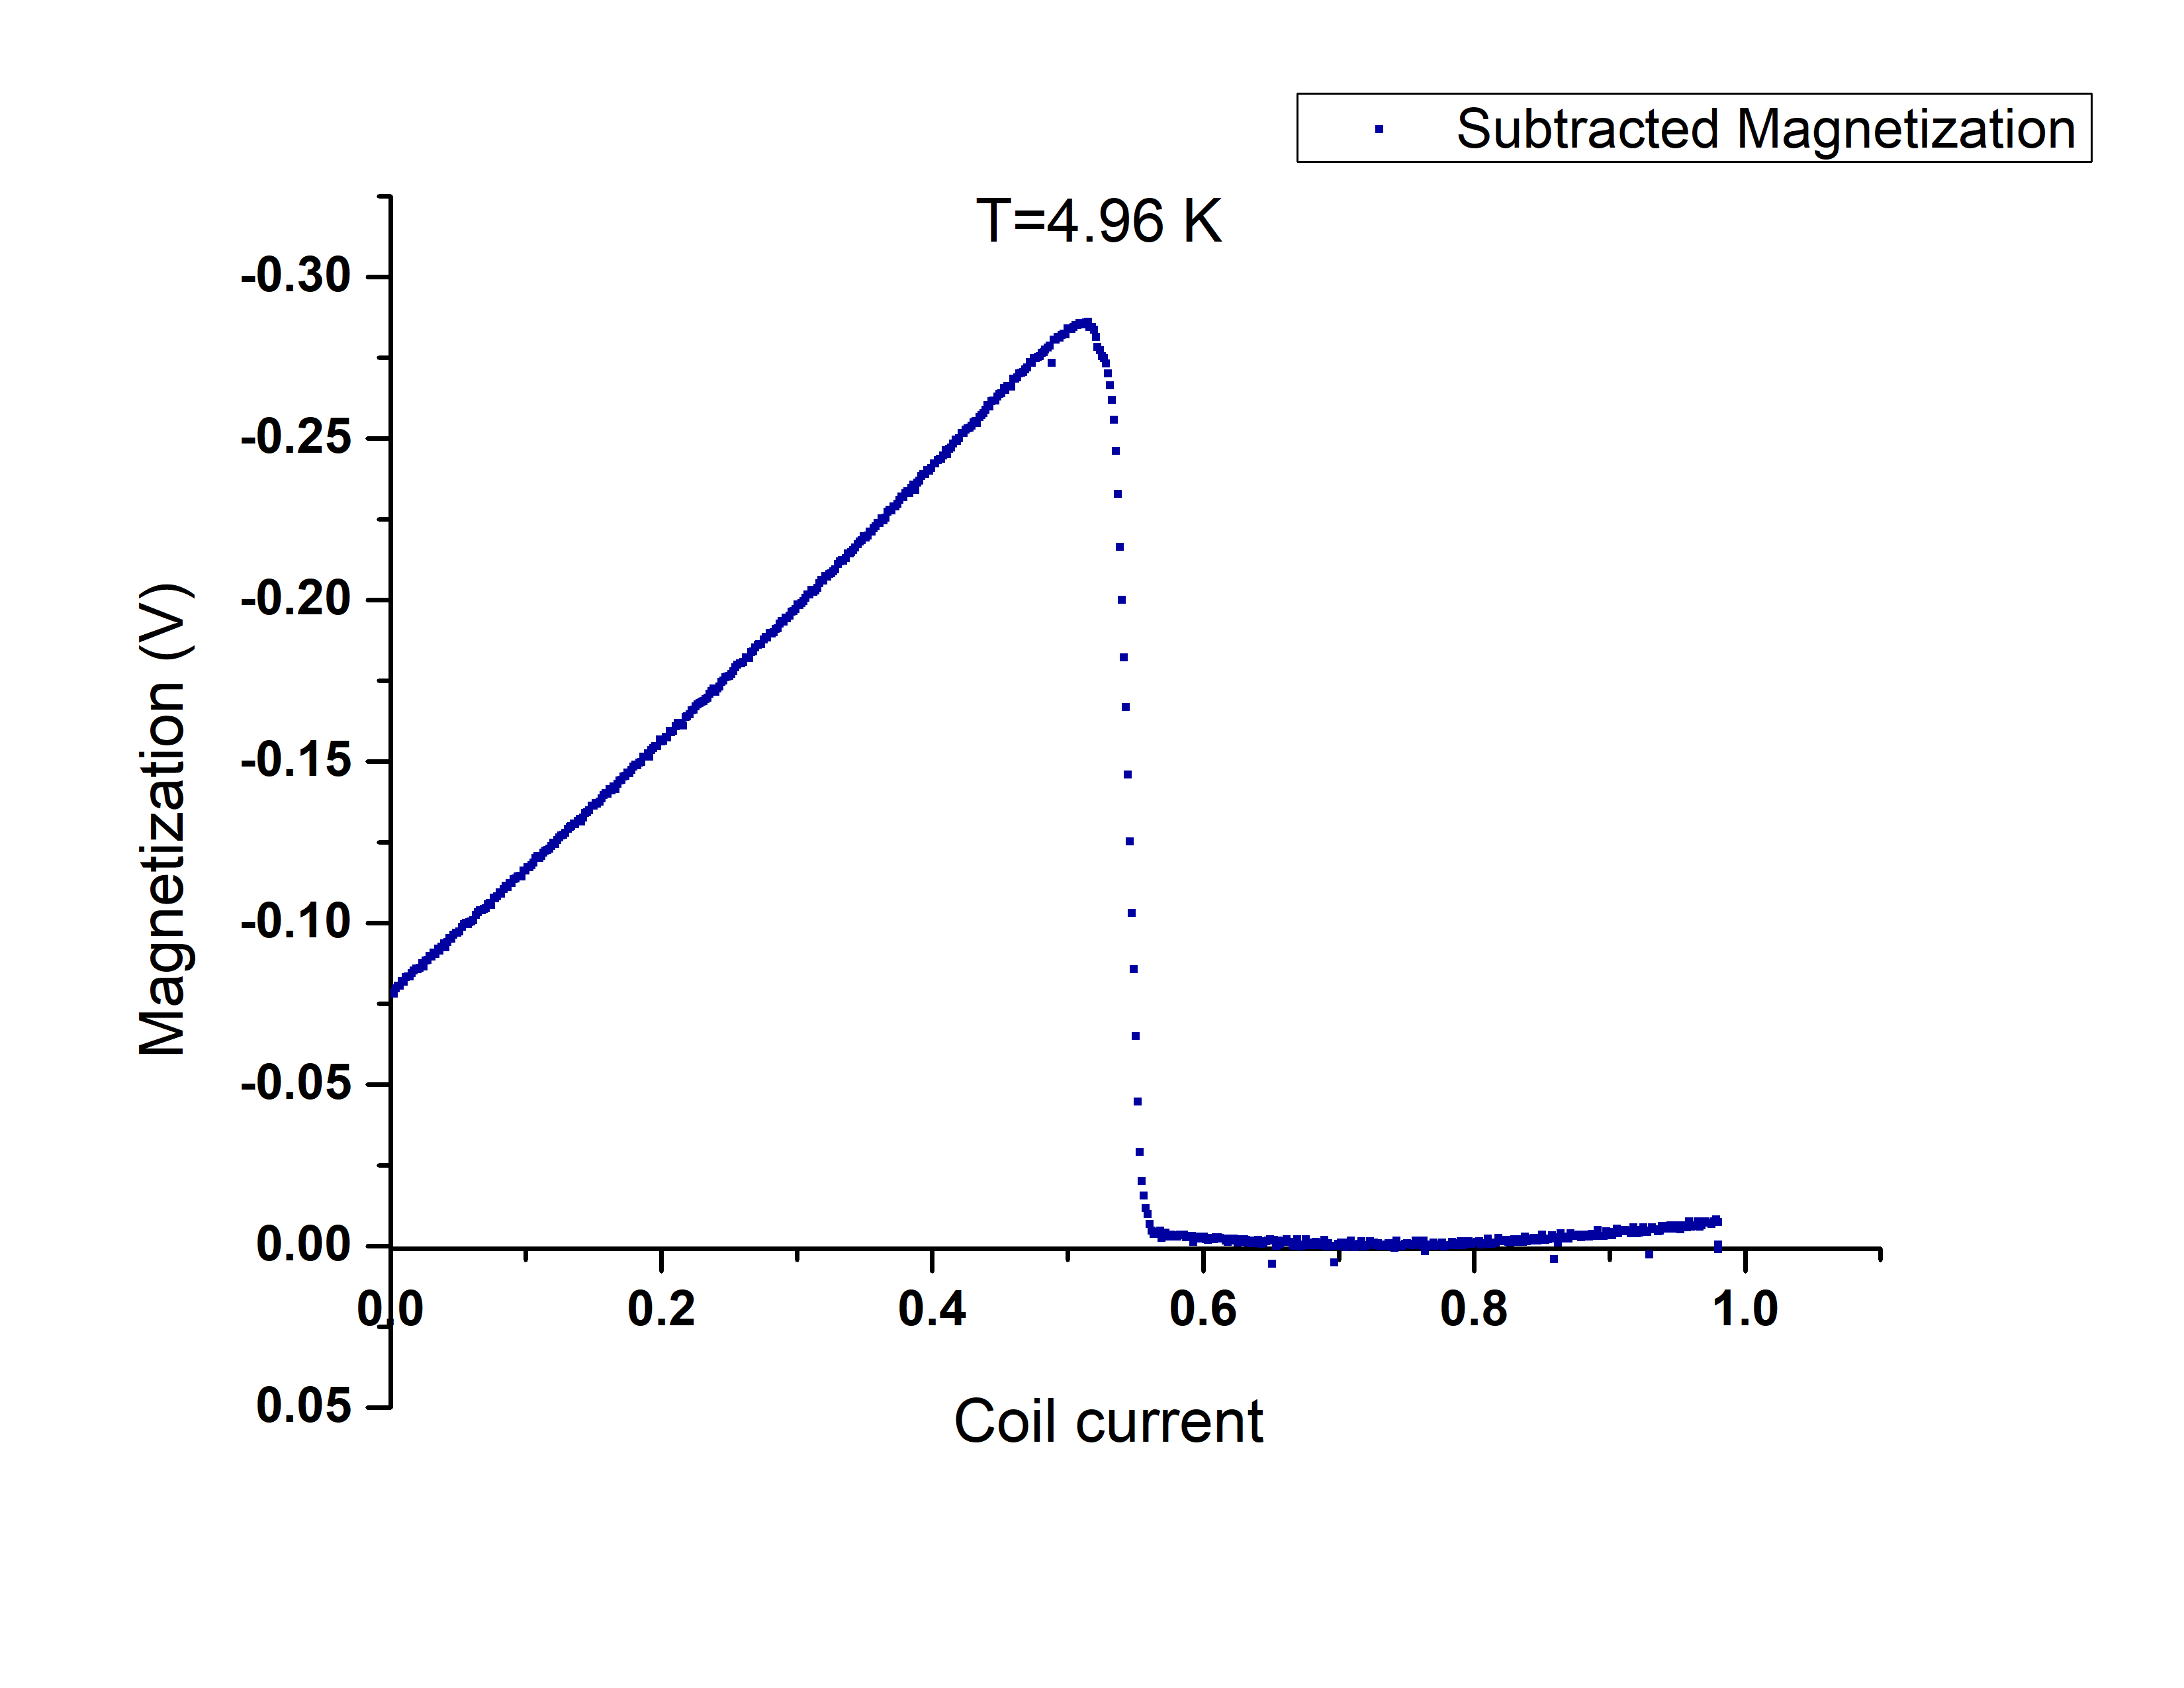
\includegraphics[scale=0.5]{496.jpg} 
\end{center}
\end{figure}


\begin{figure}[H]
\begin{center}
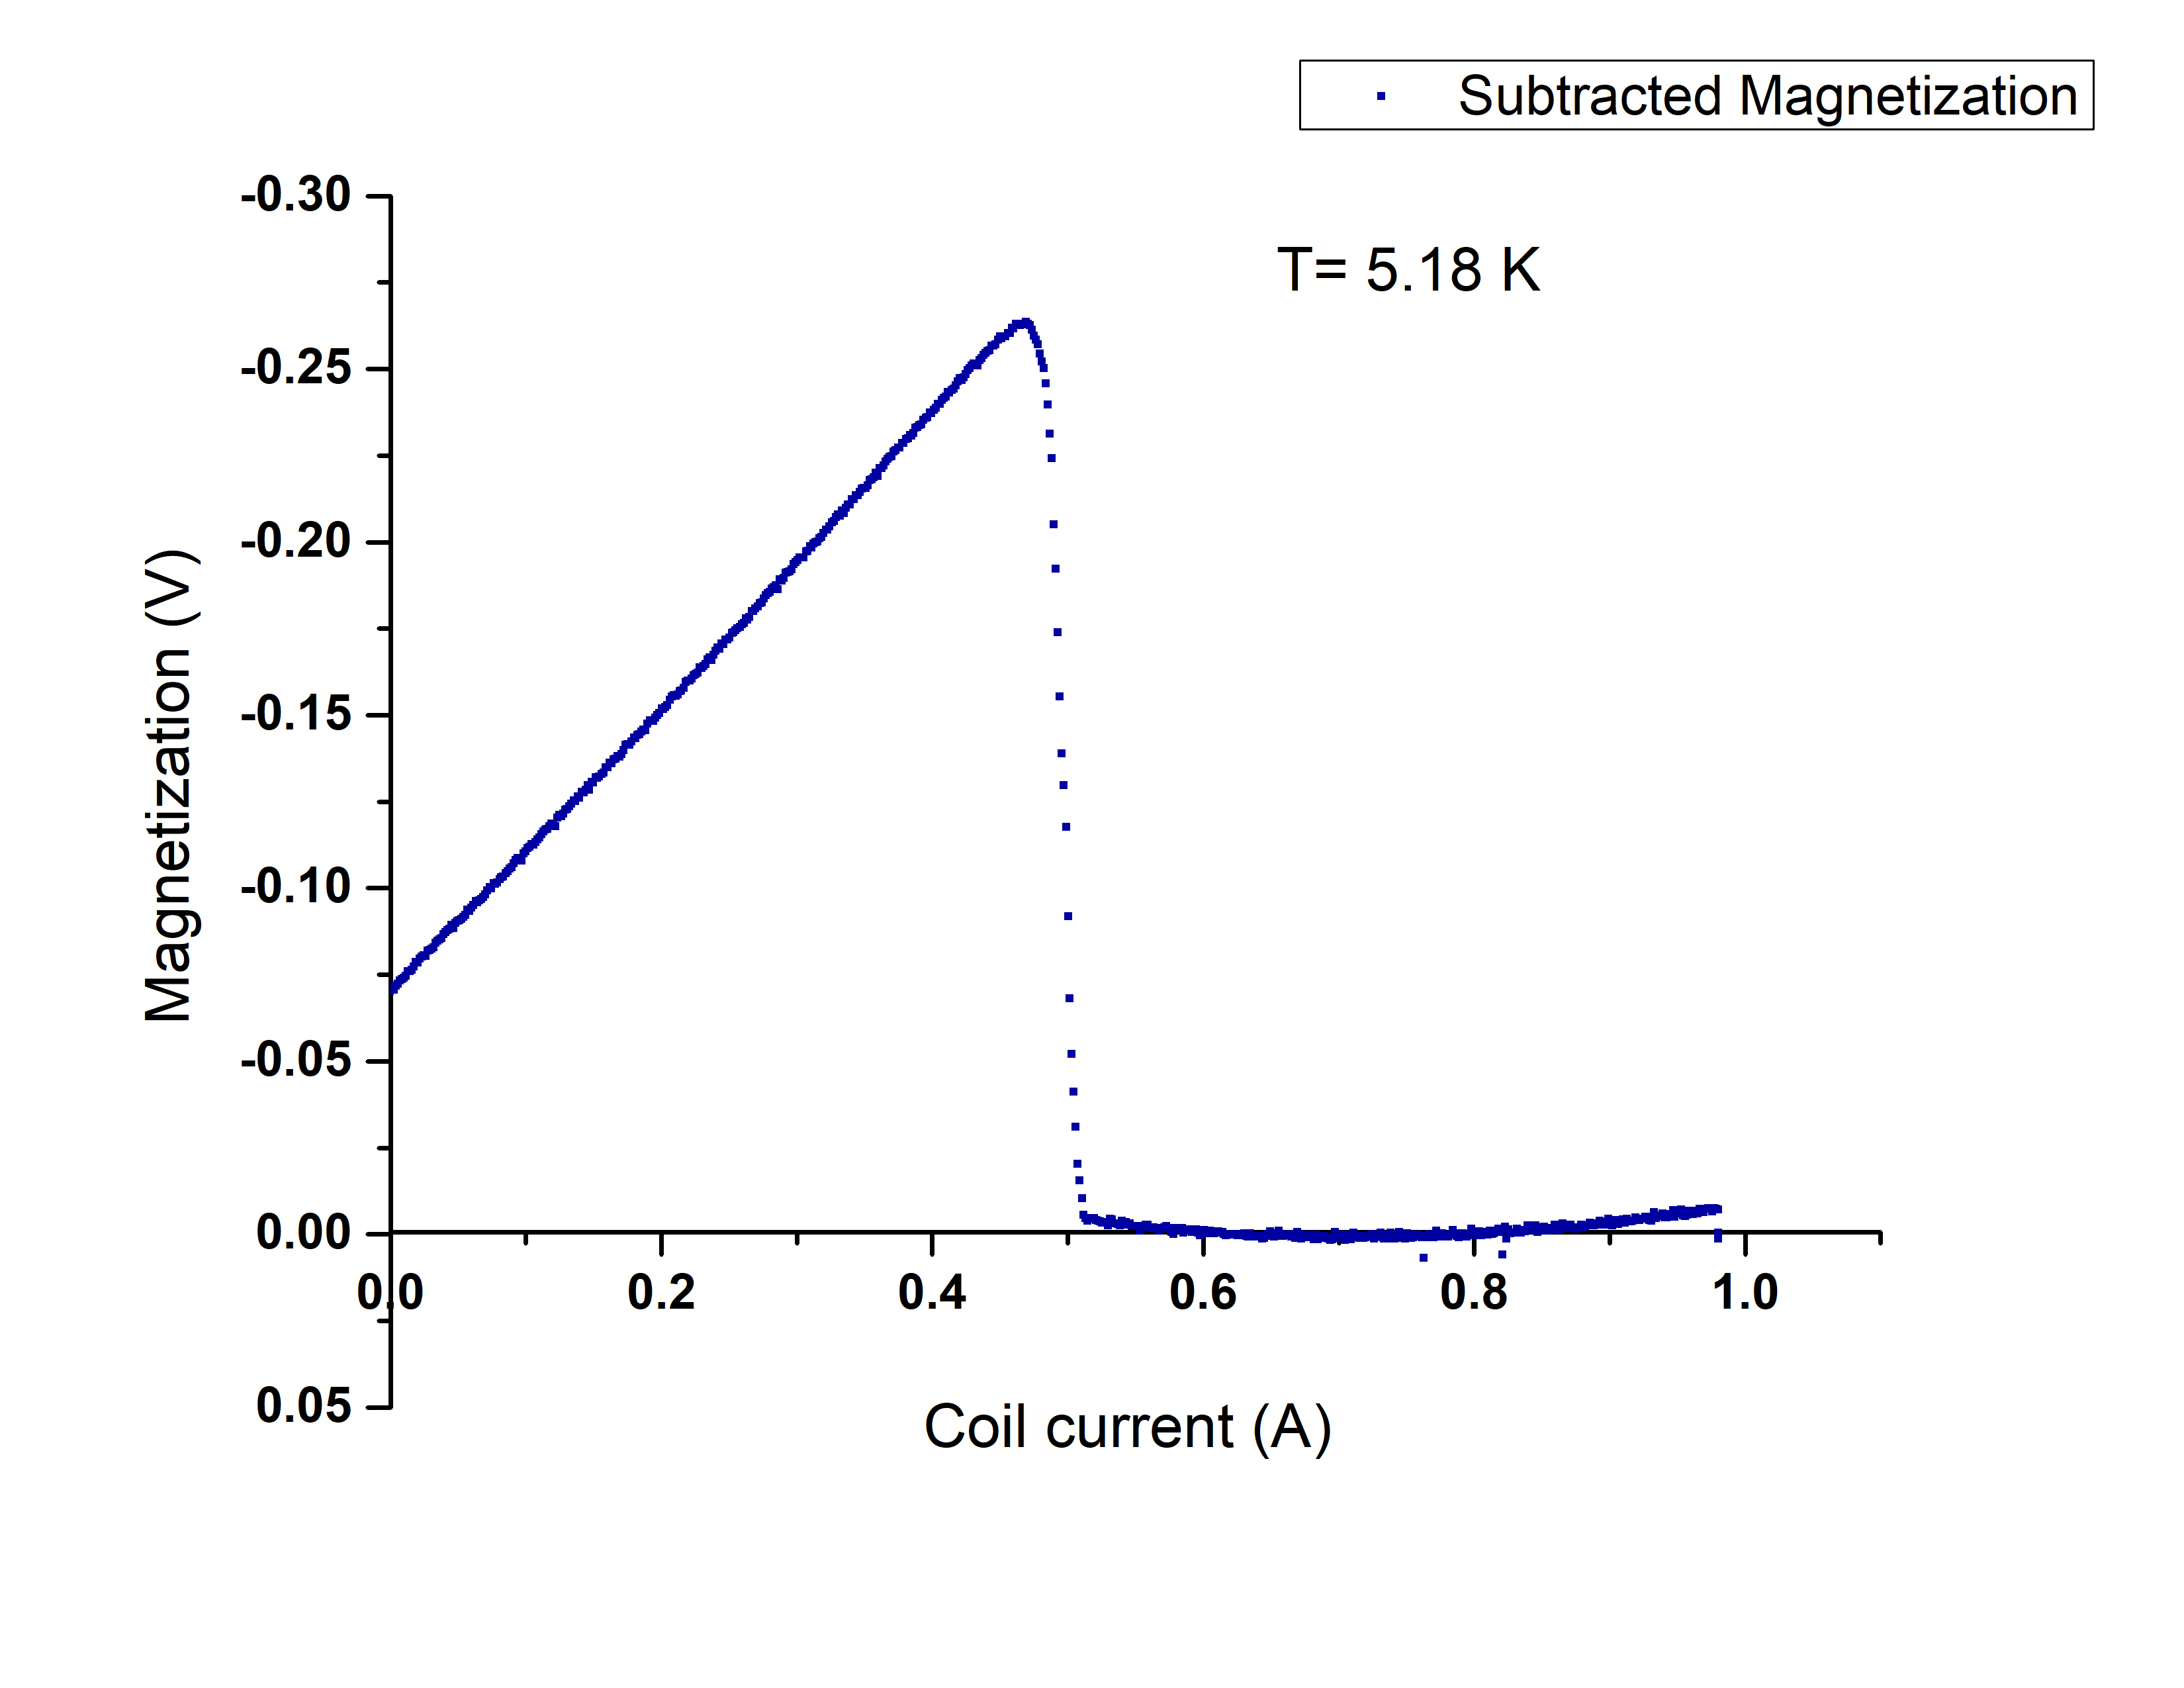
\includegraphics[scale=0.5]{518.jpg} 
\end{center}
\end{figure}

\begin{figure}[H]
\begin{center}
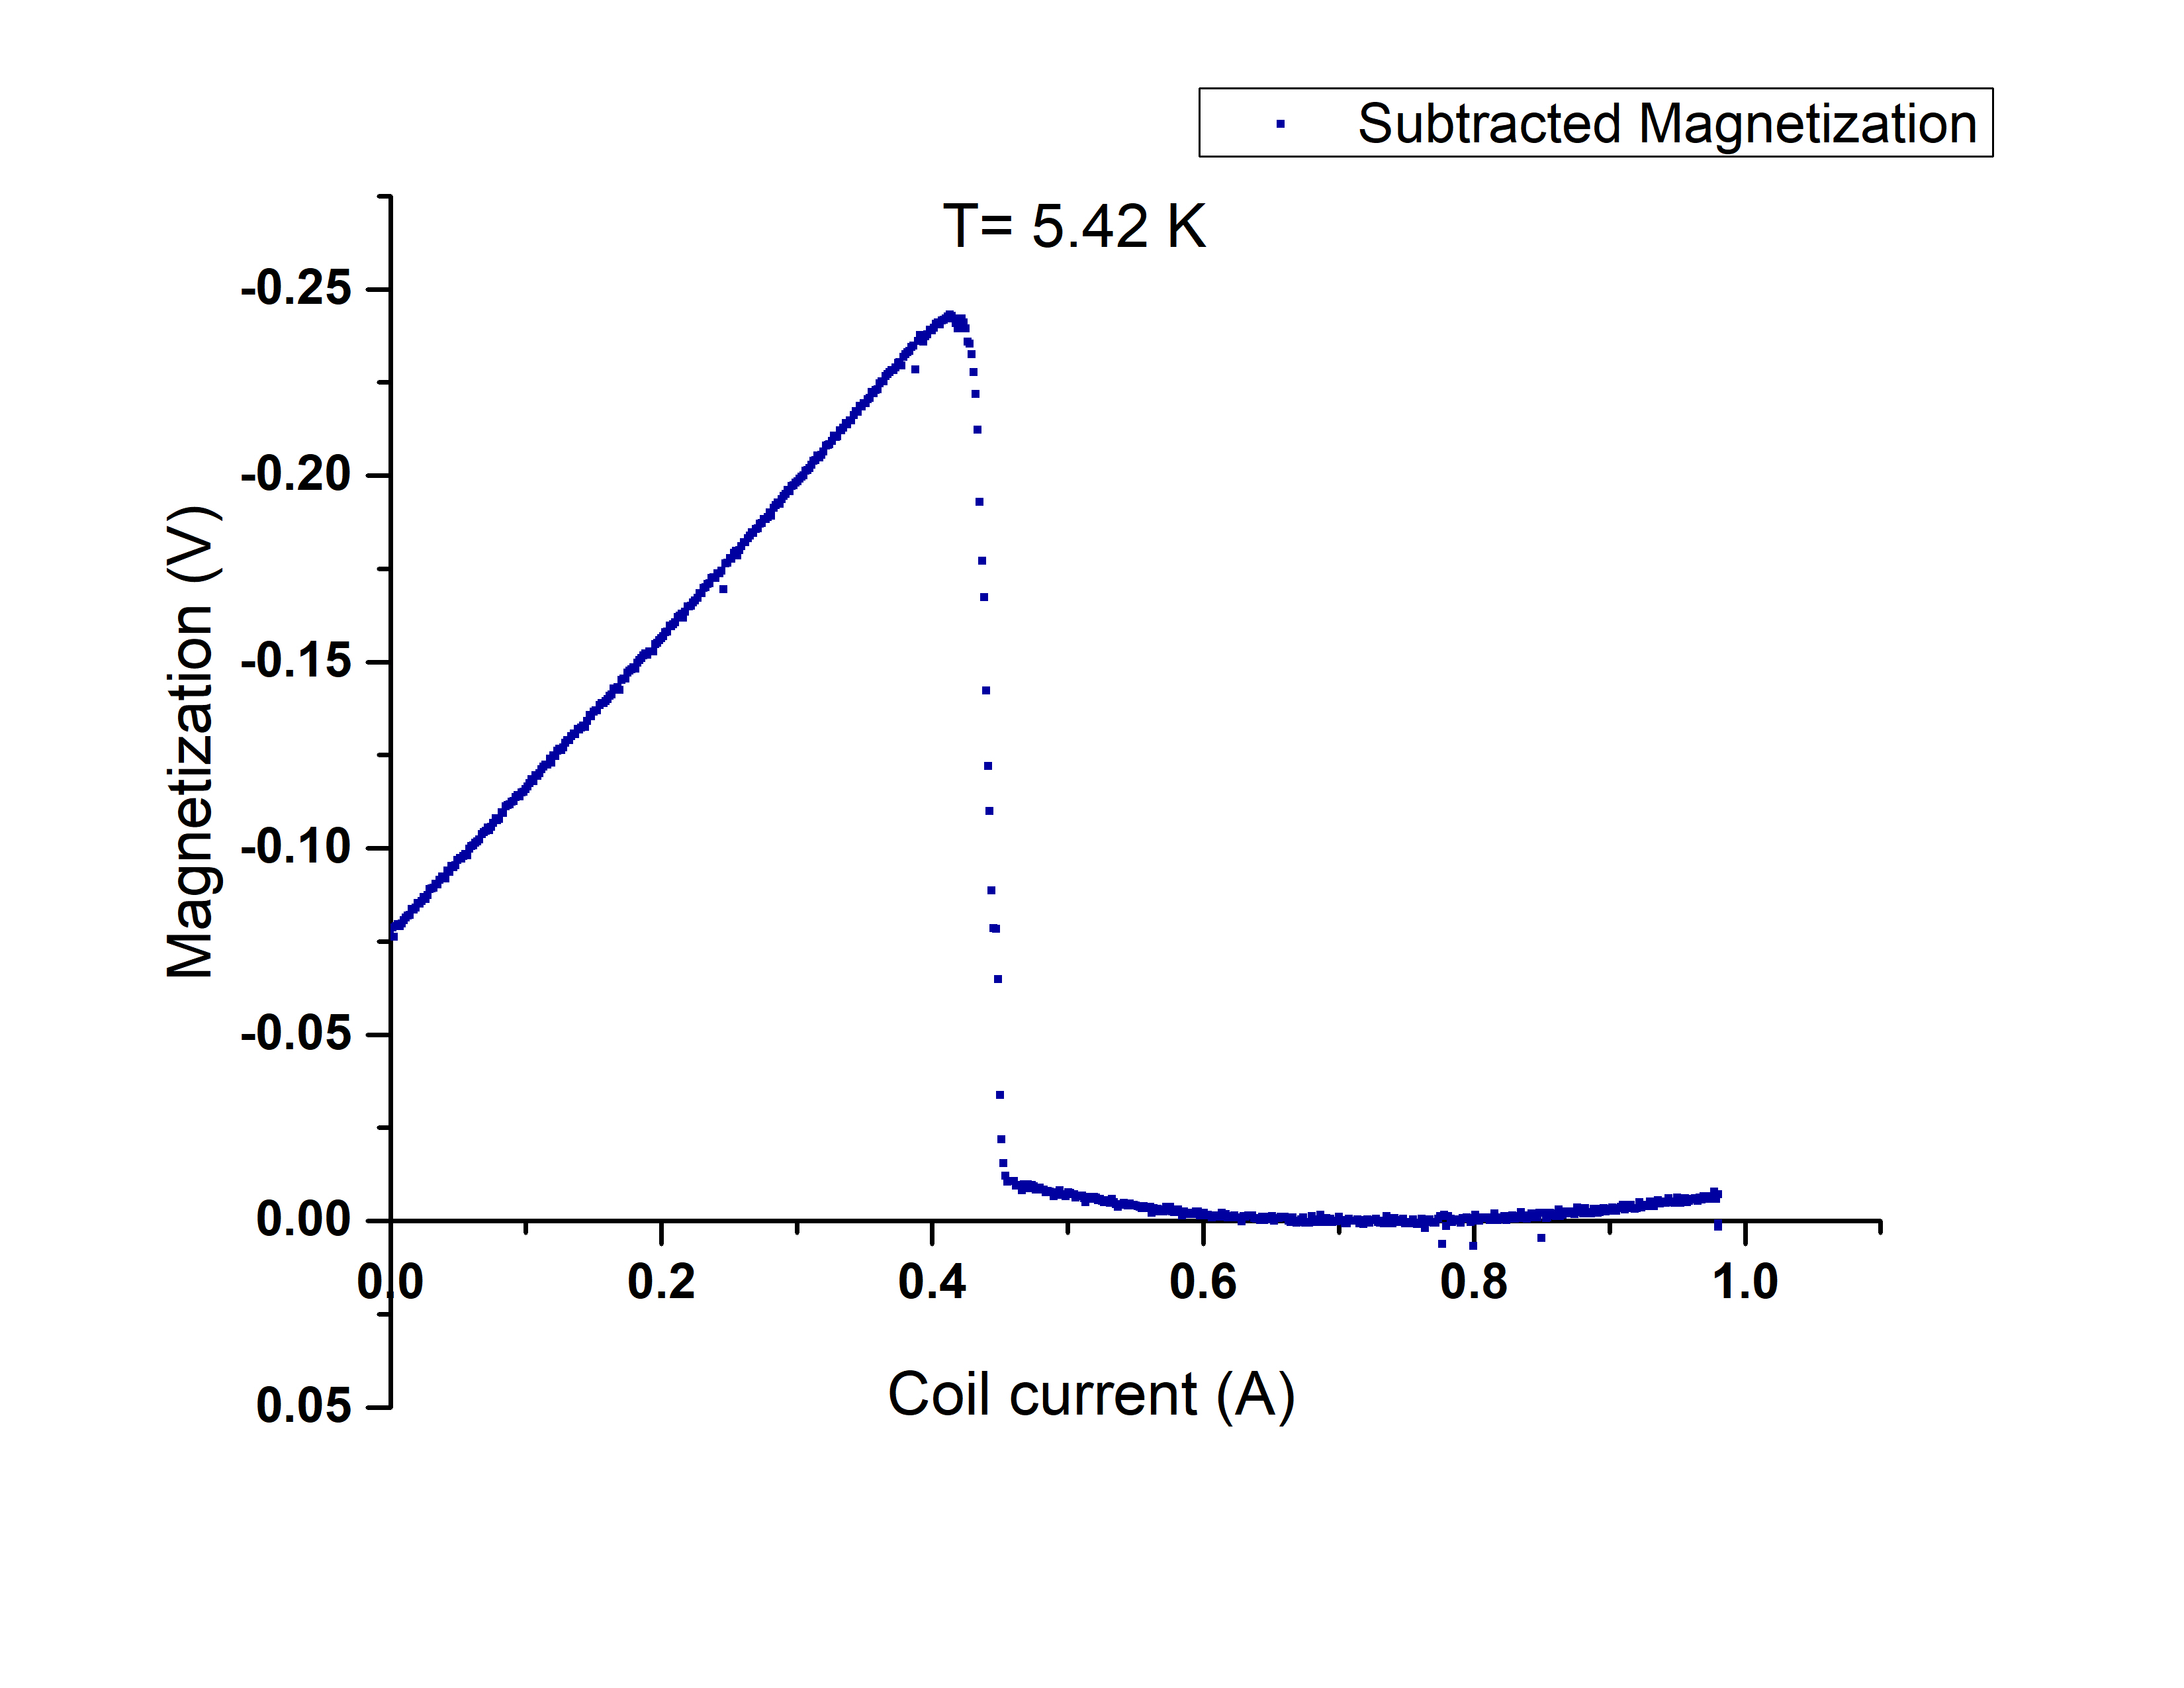
\includegraphics[scale=0.5]{542.jpg}
\end{center}
\end{figure}

\begin{figure}[H]
\begin{center}
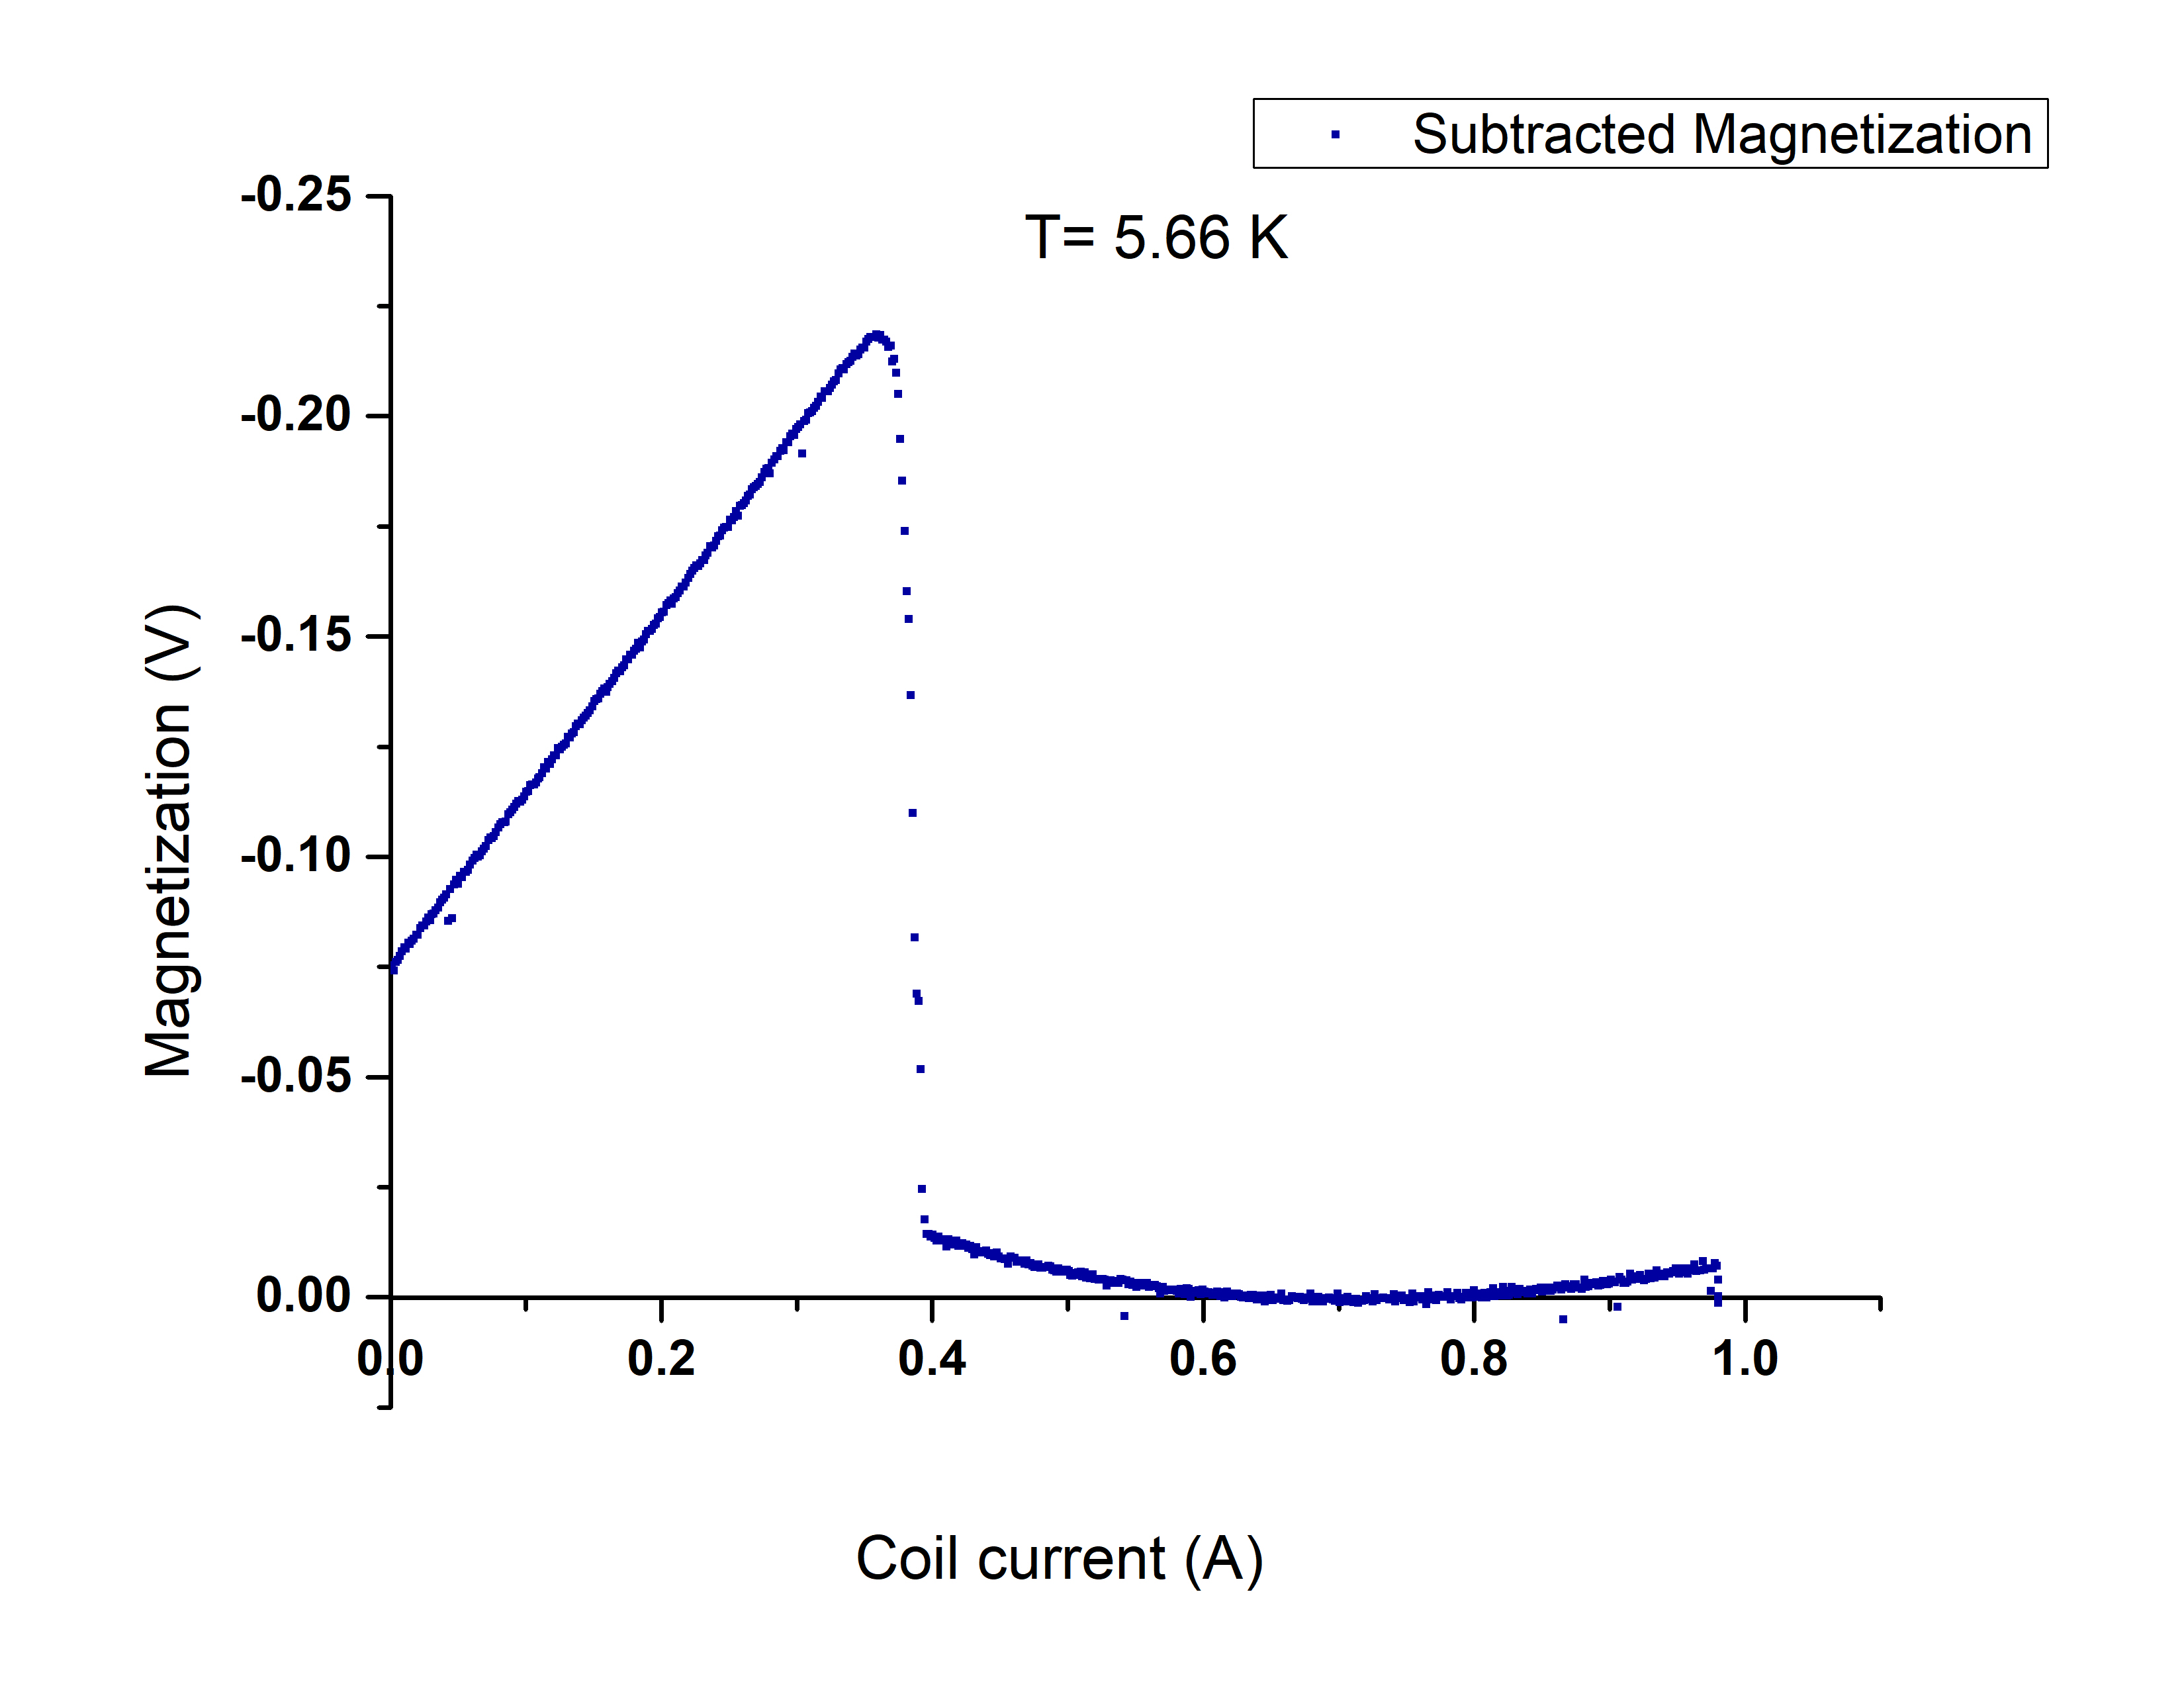
\includegraphics[scale=0.5]{566.jpg}
\end{center}
\end{figure}


\begin{figure}[H]
\begin{center}
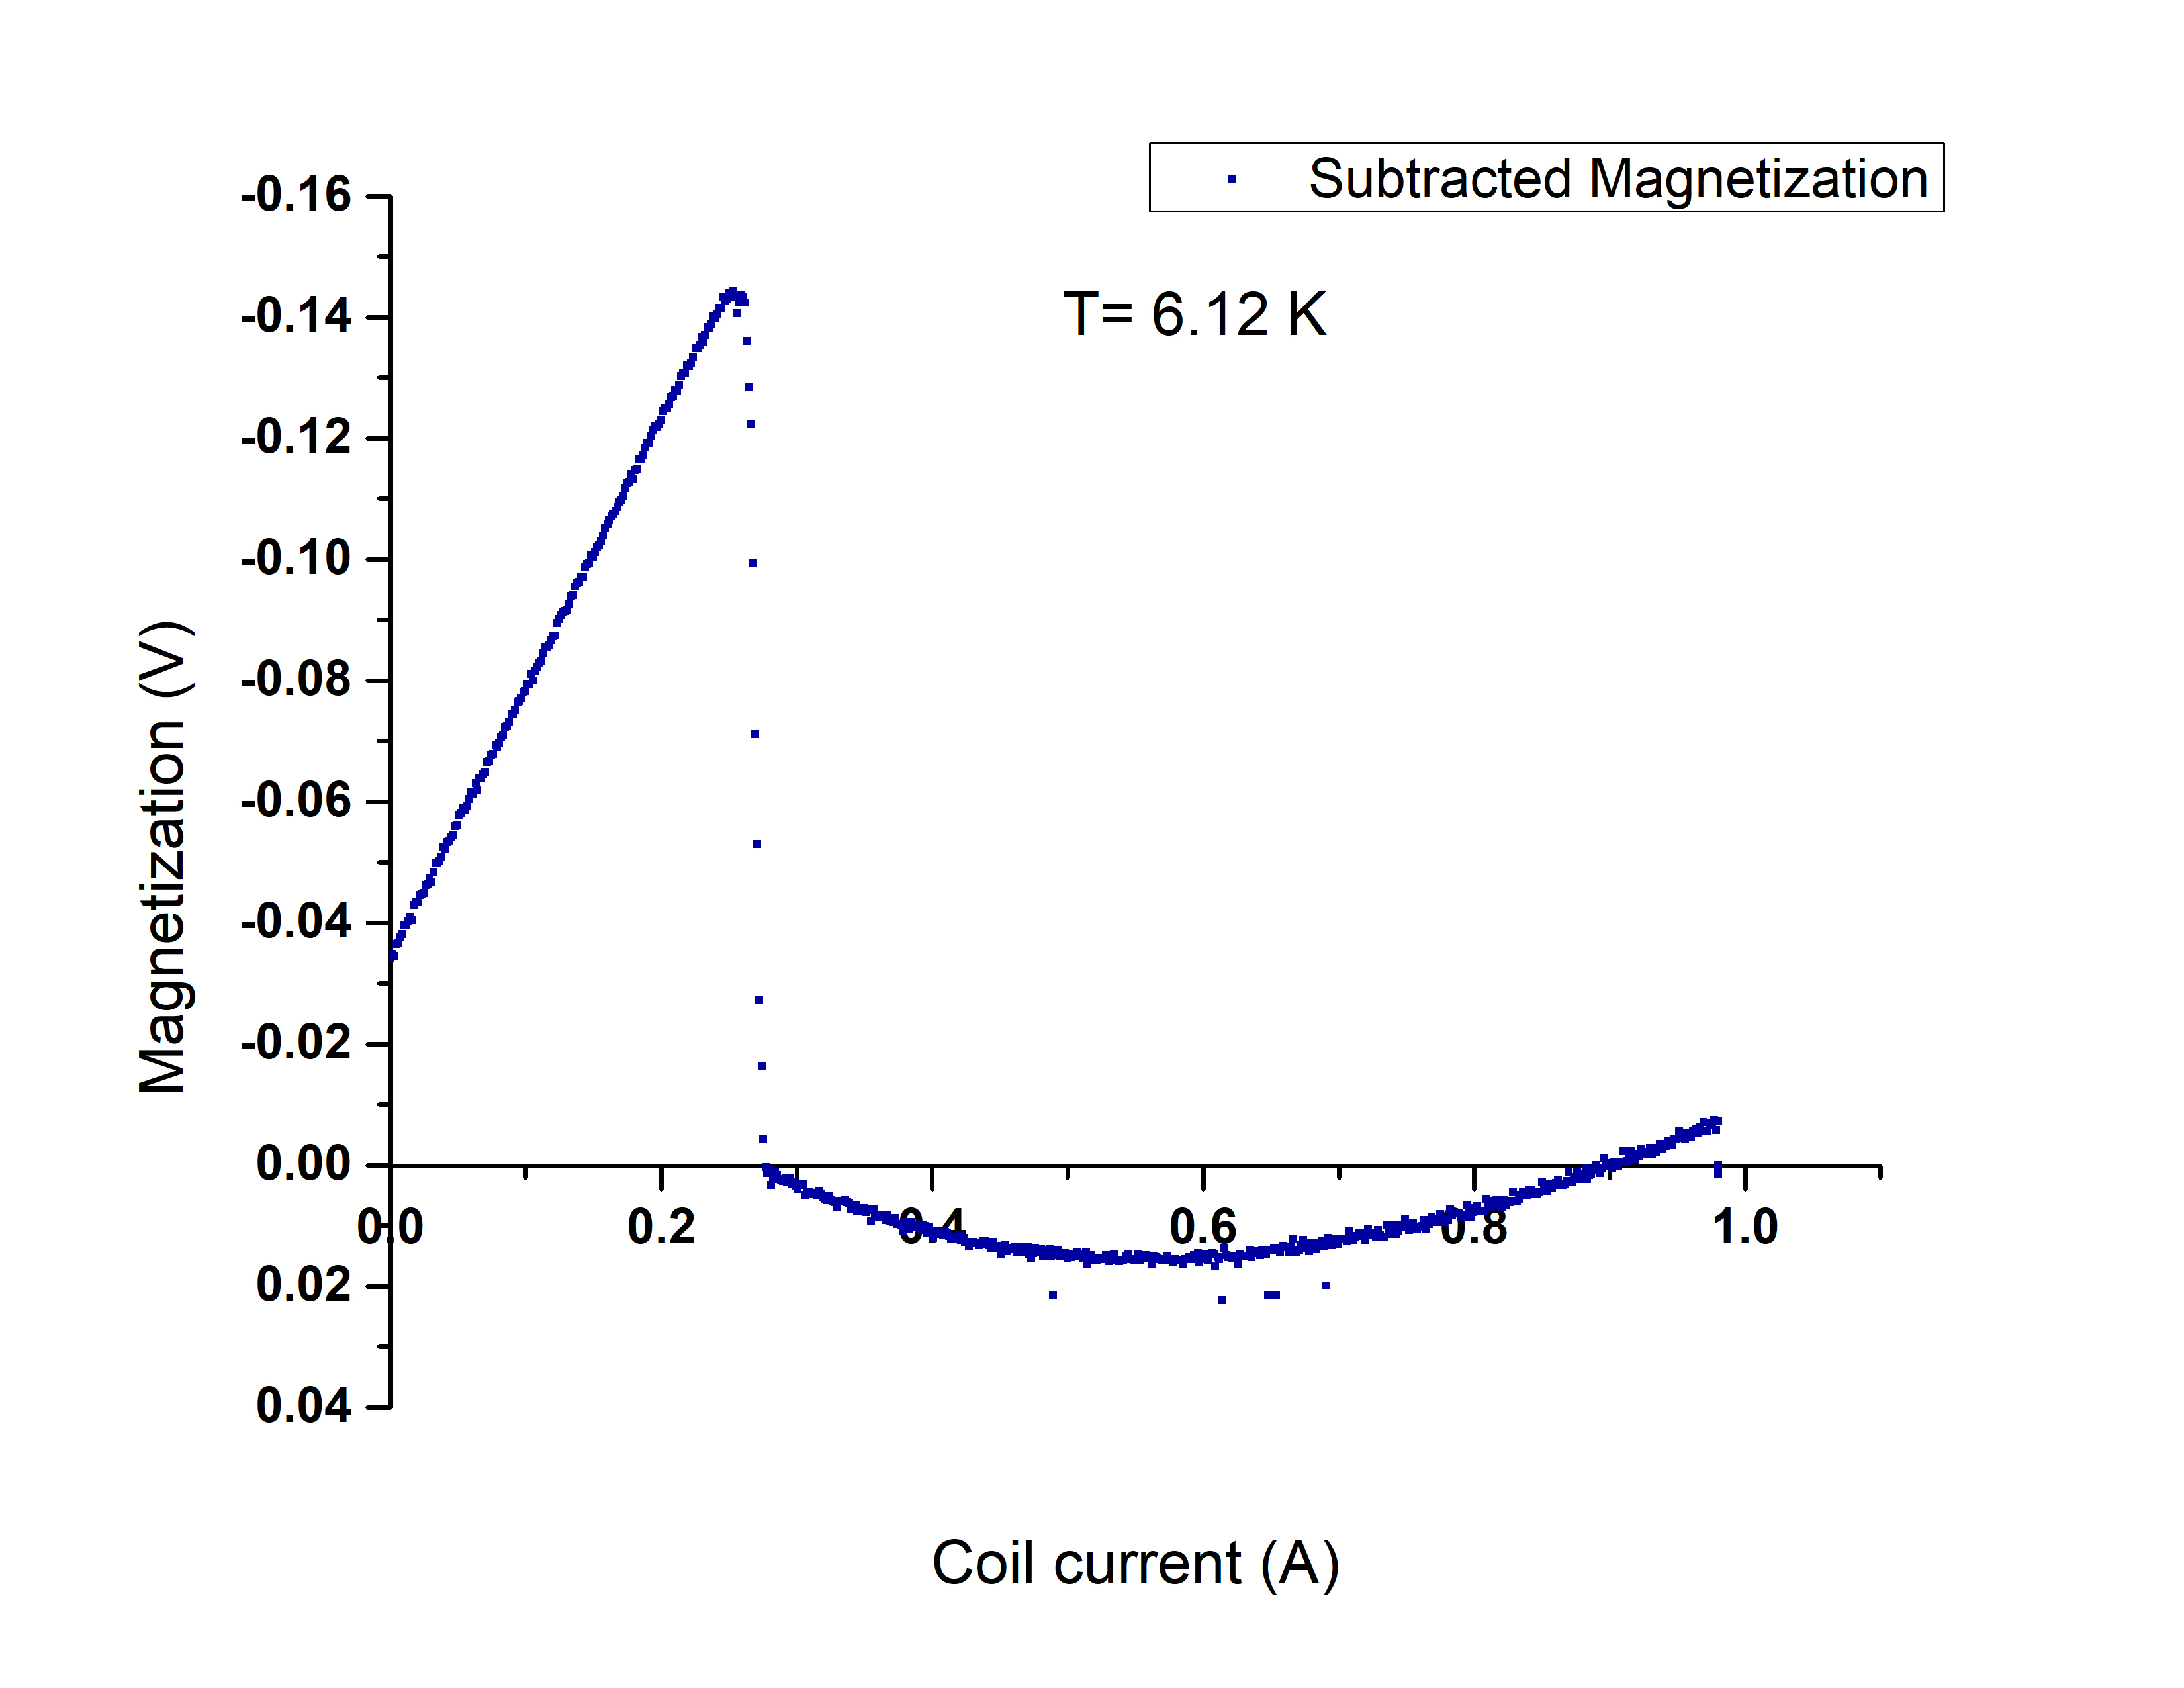
\includegraphics[scale=0.45]{612.jpg} 
\end{center}
\end{figure}



\begin{figure}[H]
\begin{center}
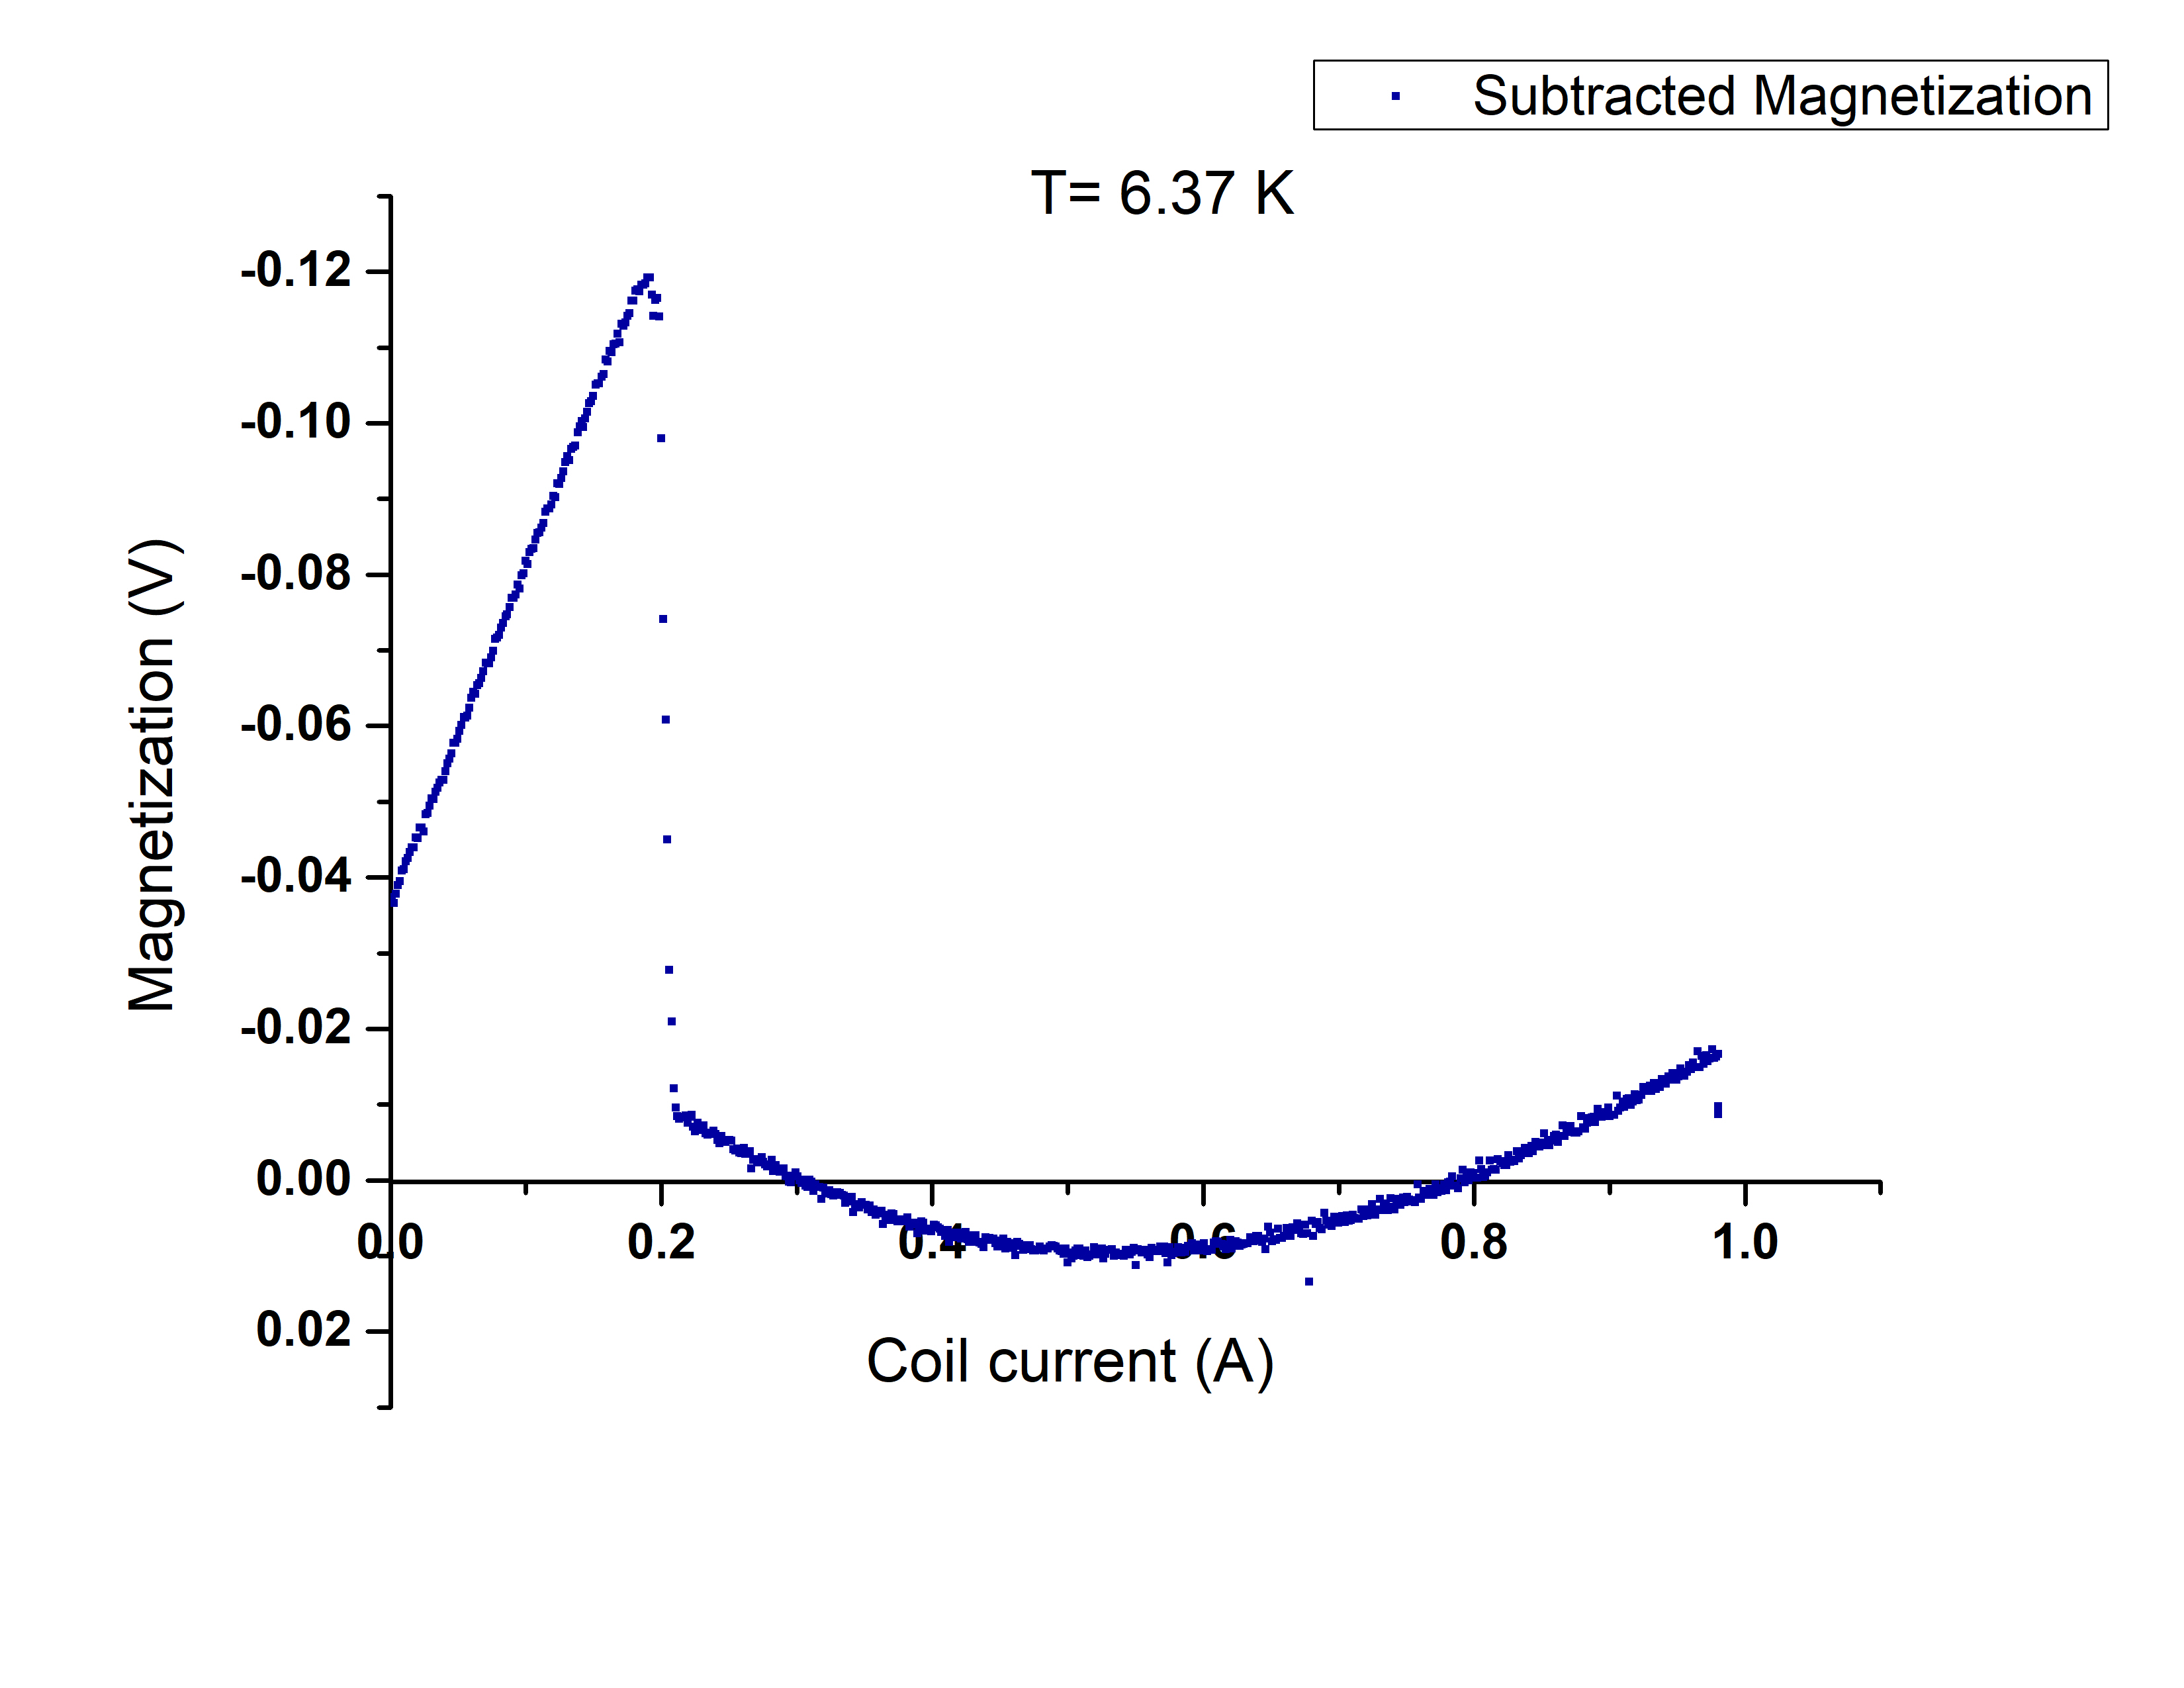
\includegraphics[scale=0.5]{637.jpg} 
\end{center}
\end{figure}


\begin{figure}[H]
\begin{center}
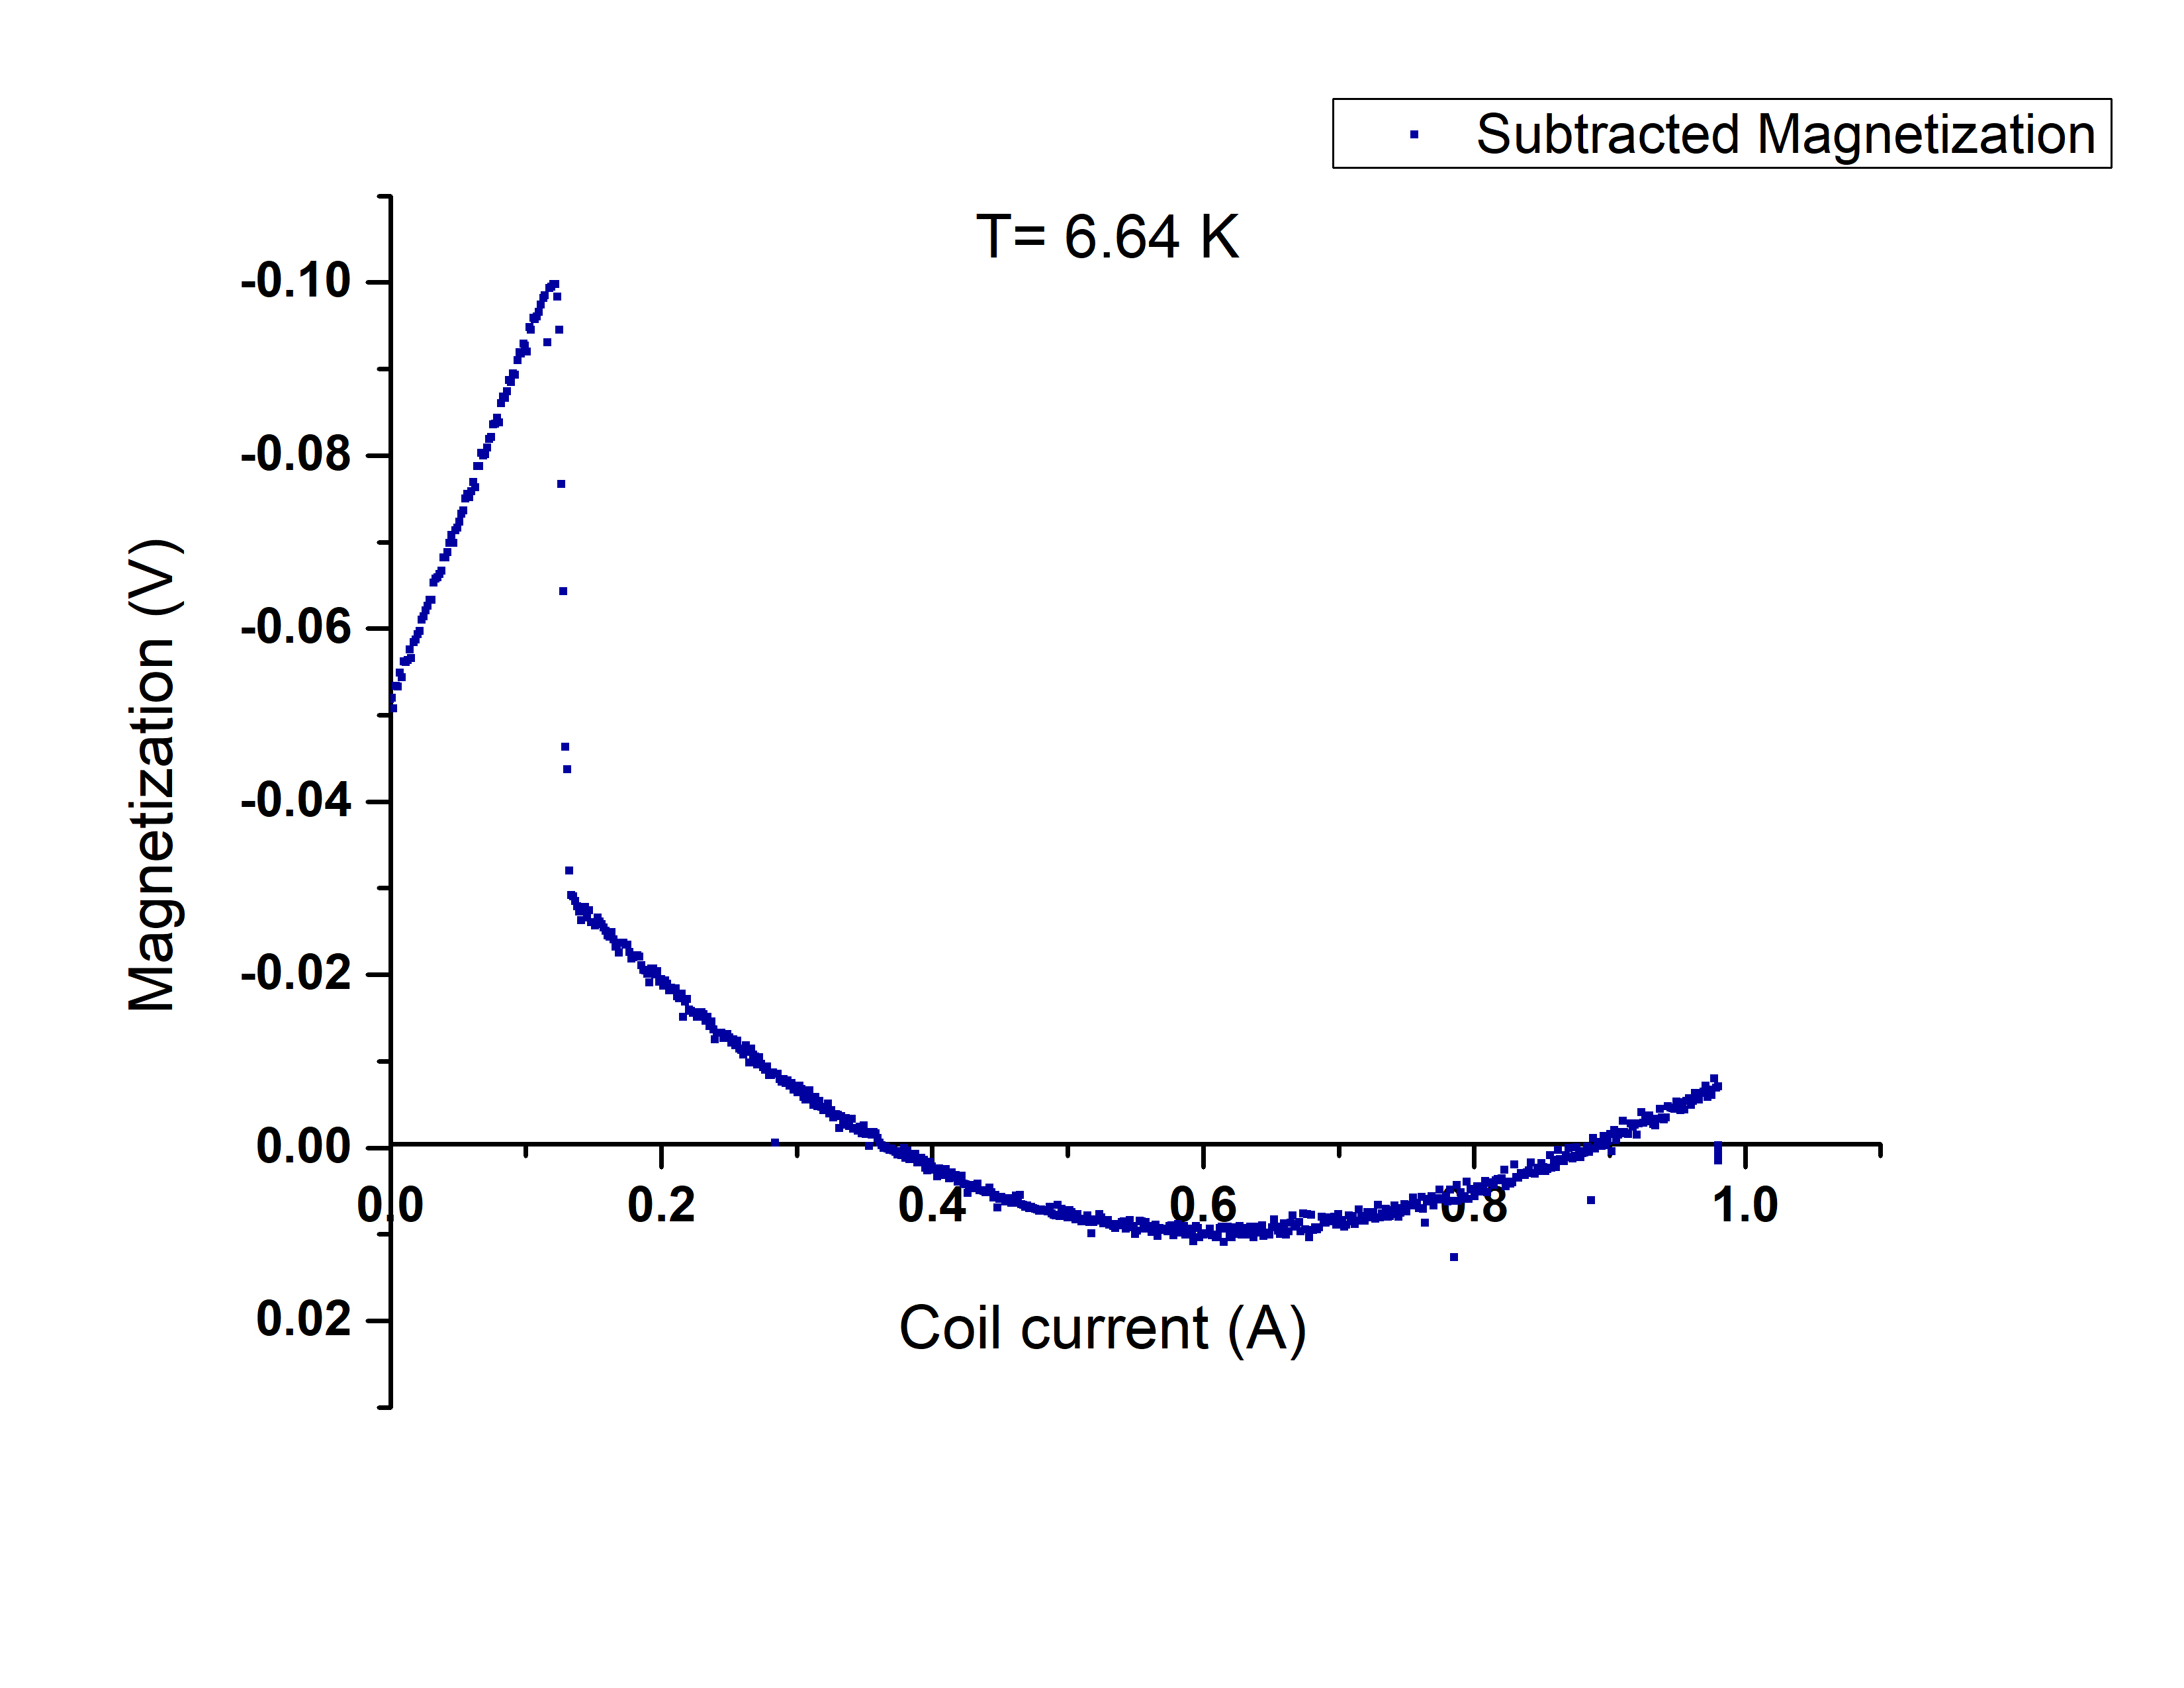
\includegraphics[scale=0.5]{664.jpg}
\end{center}
\end{figure}

\begin{figure}[H]
\begin{center}
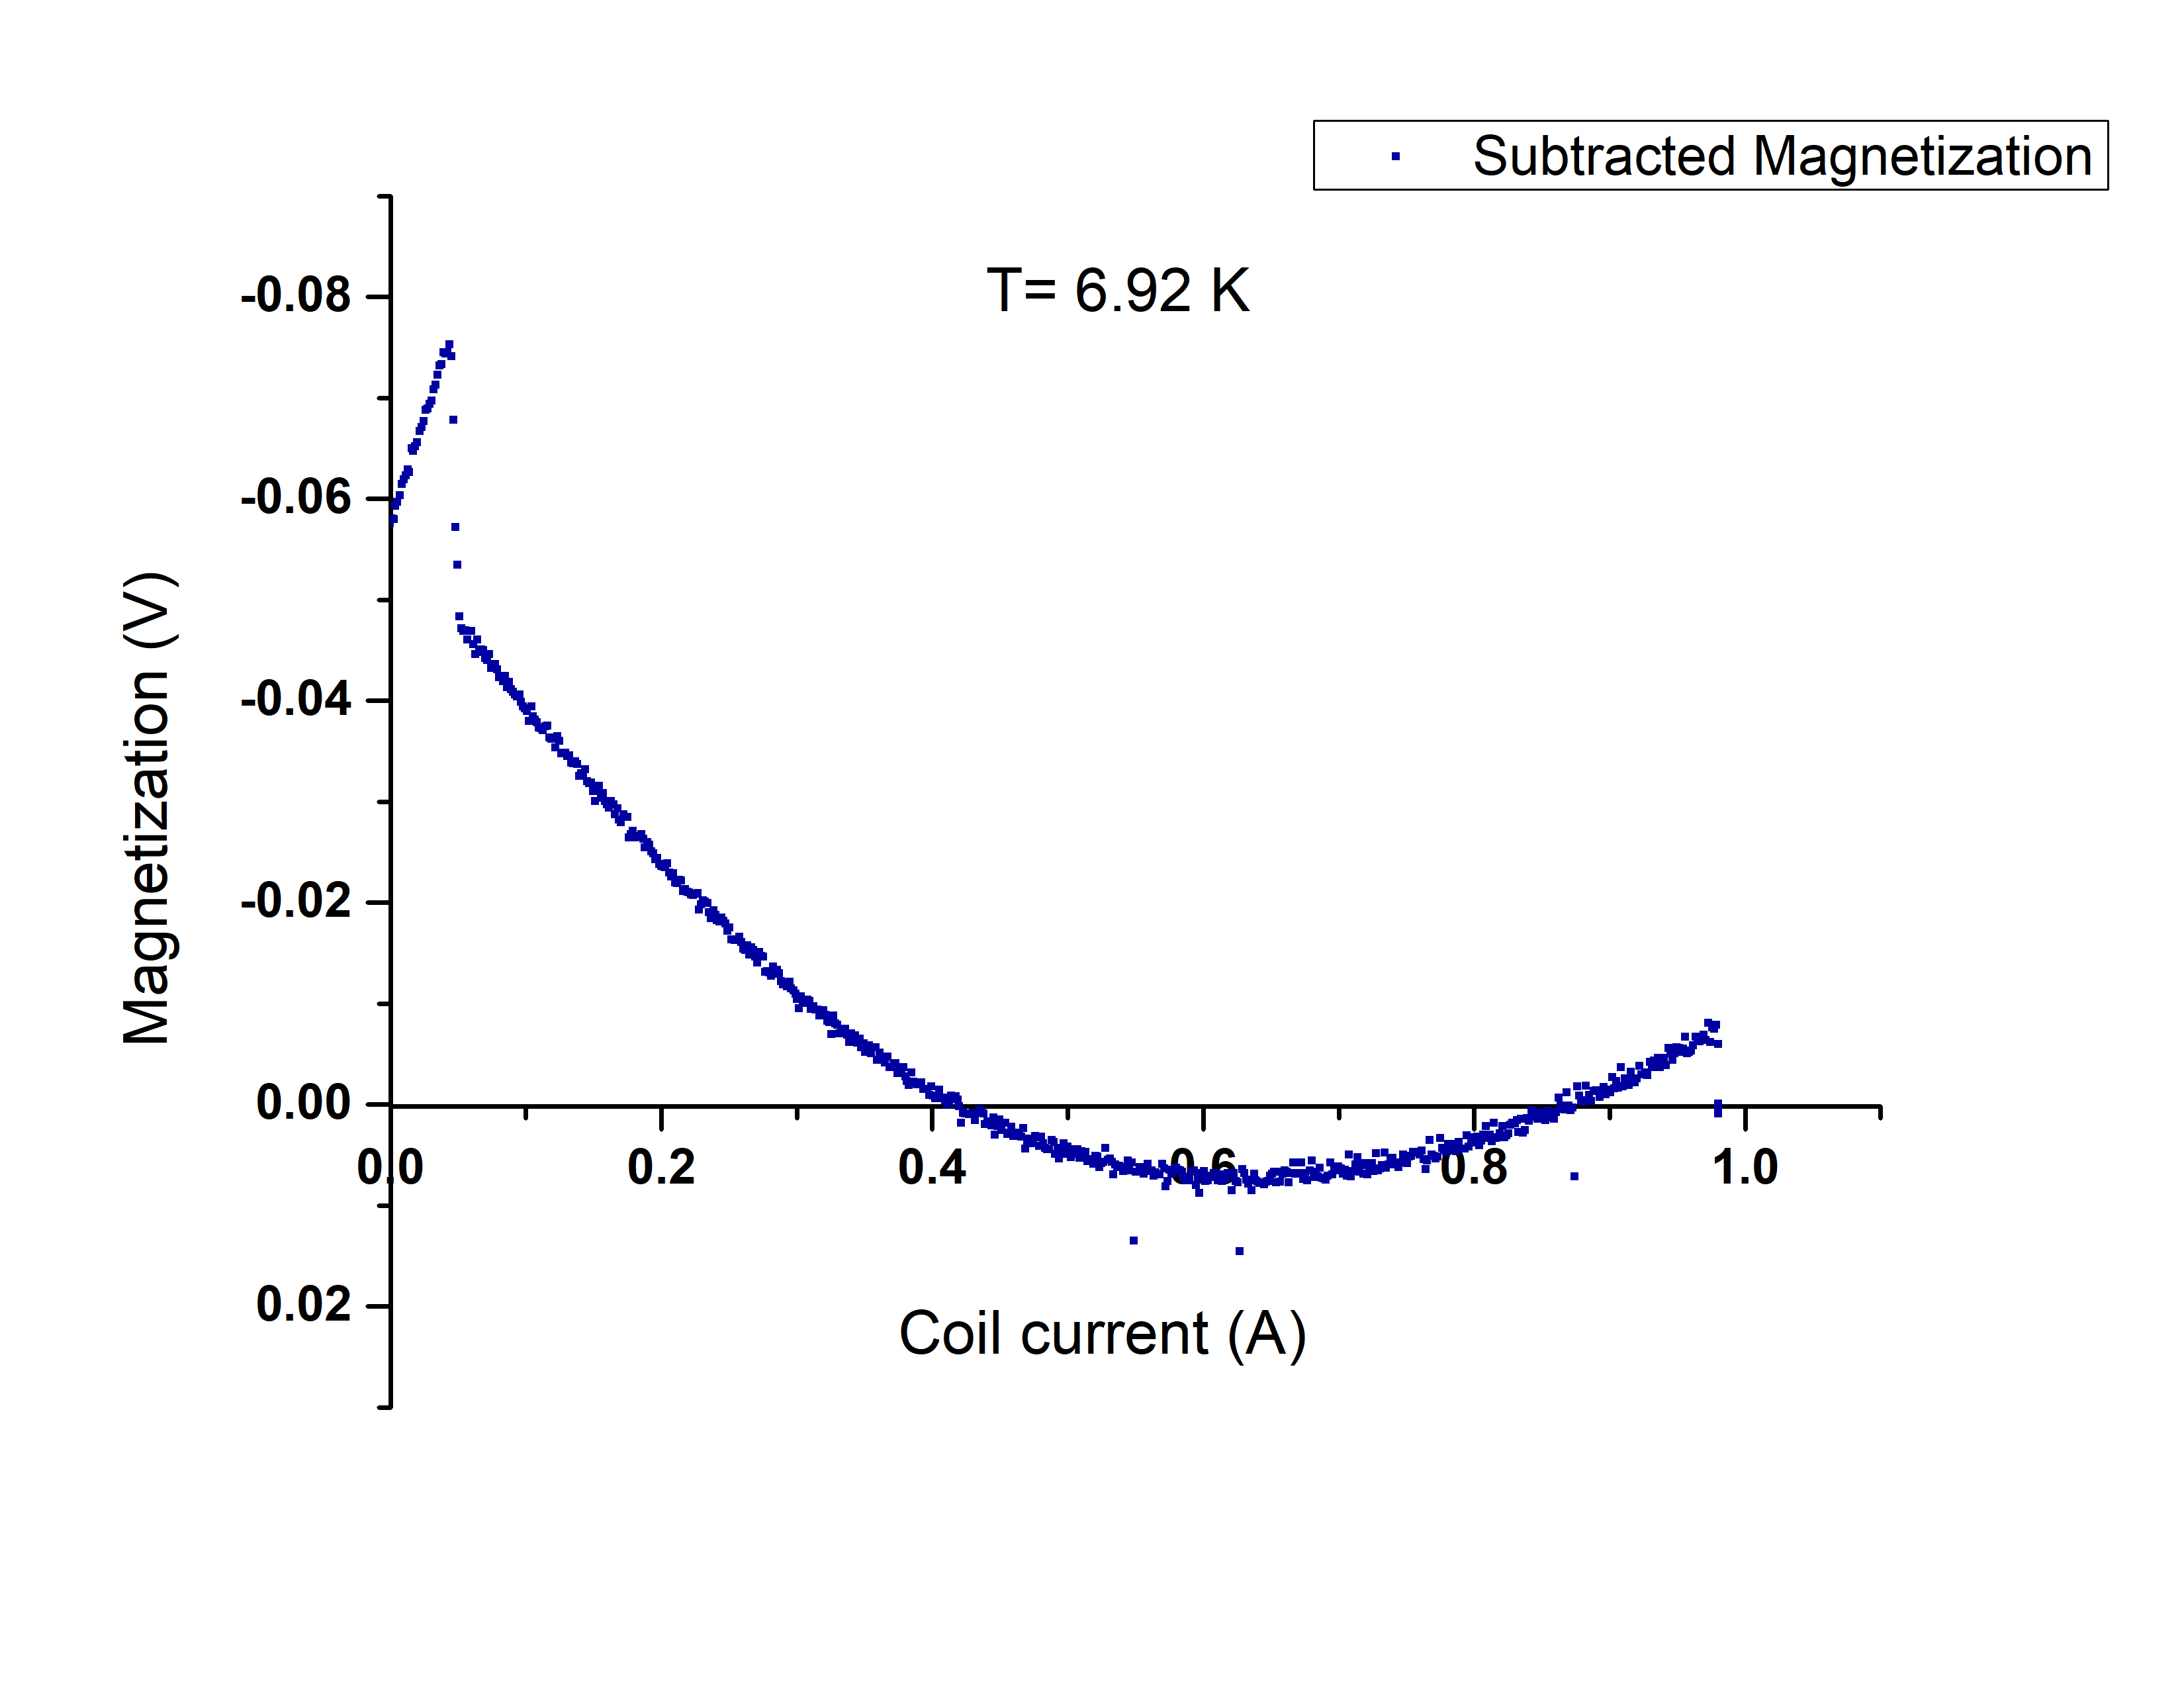
\includegraphics[scale=0.5]{692.jpg}
\end{center}
\end{figure}

\begin{figure}[H]
\begin{center}
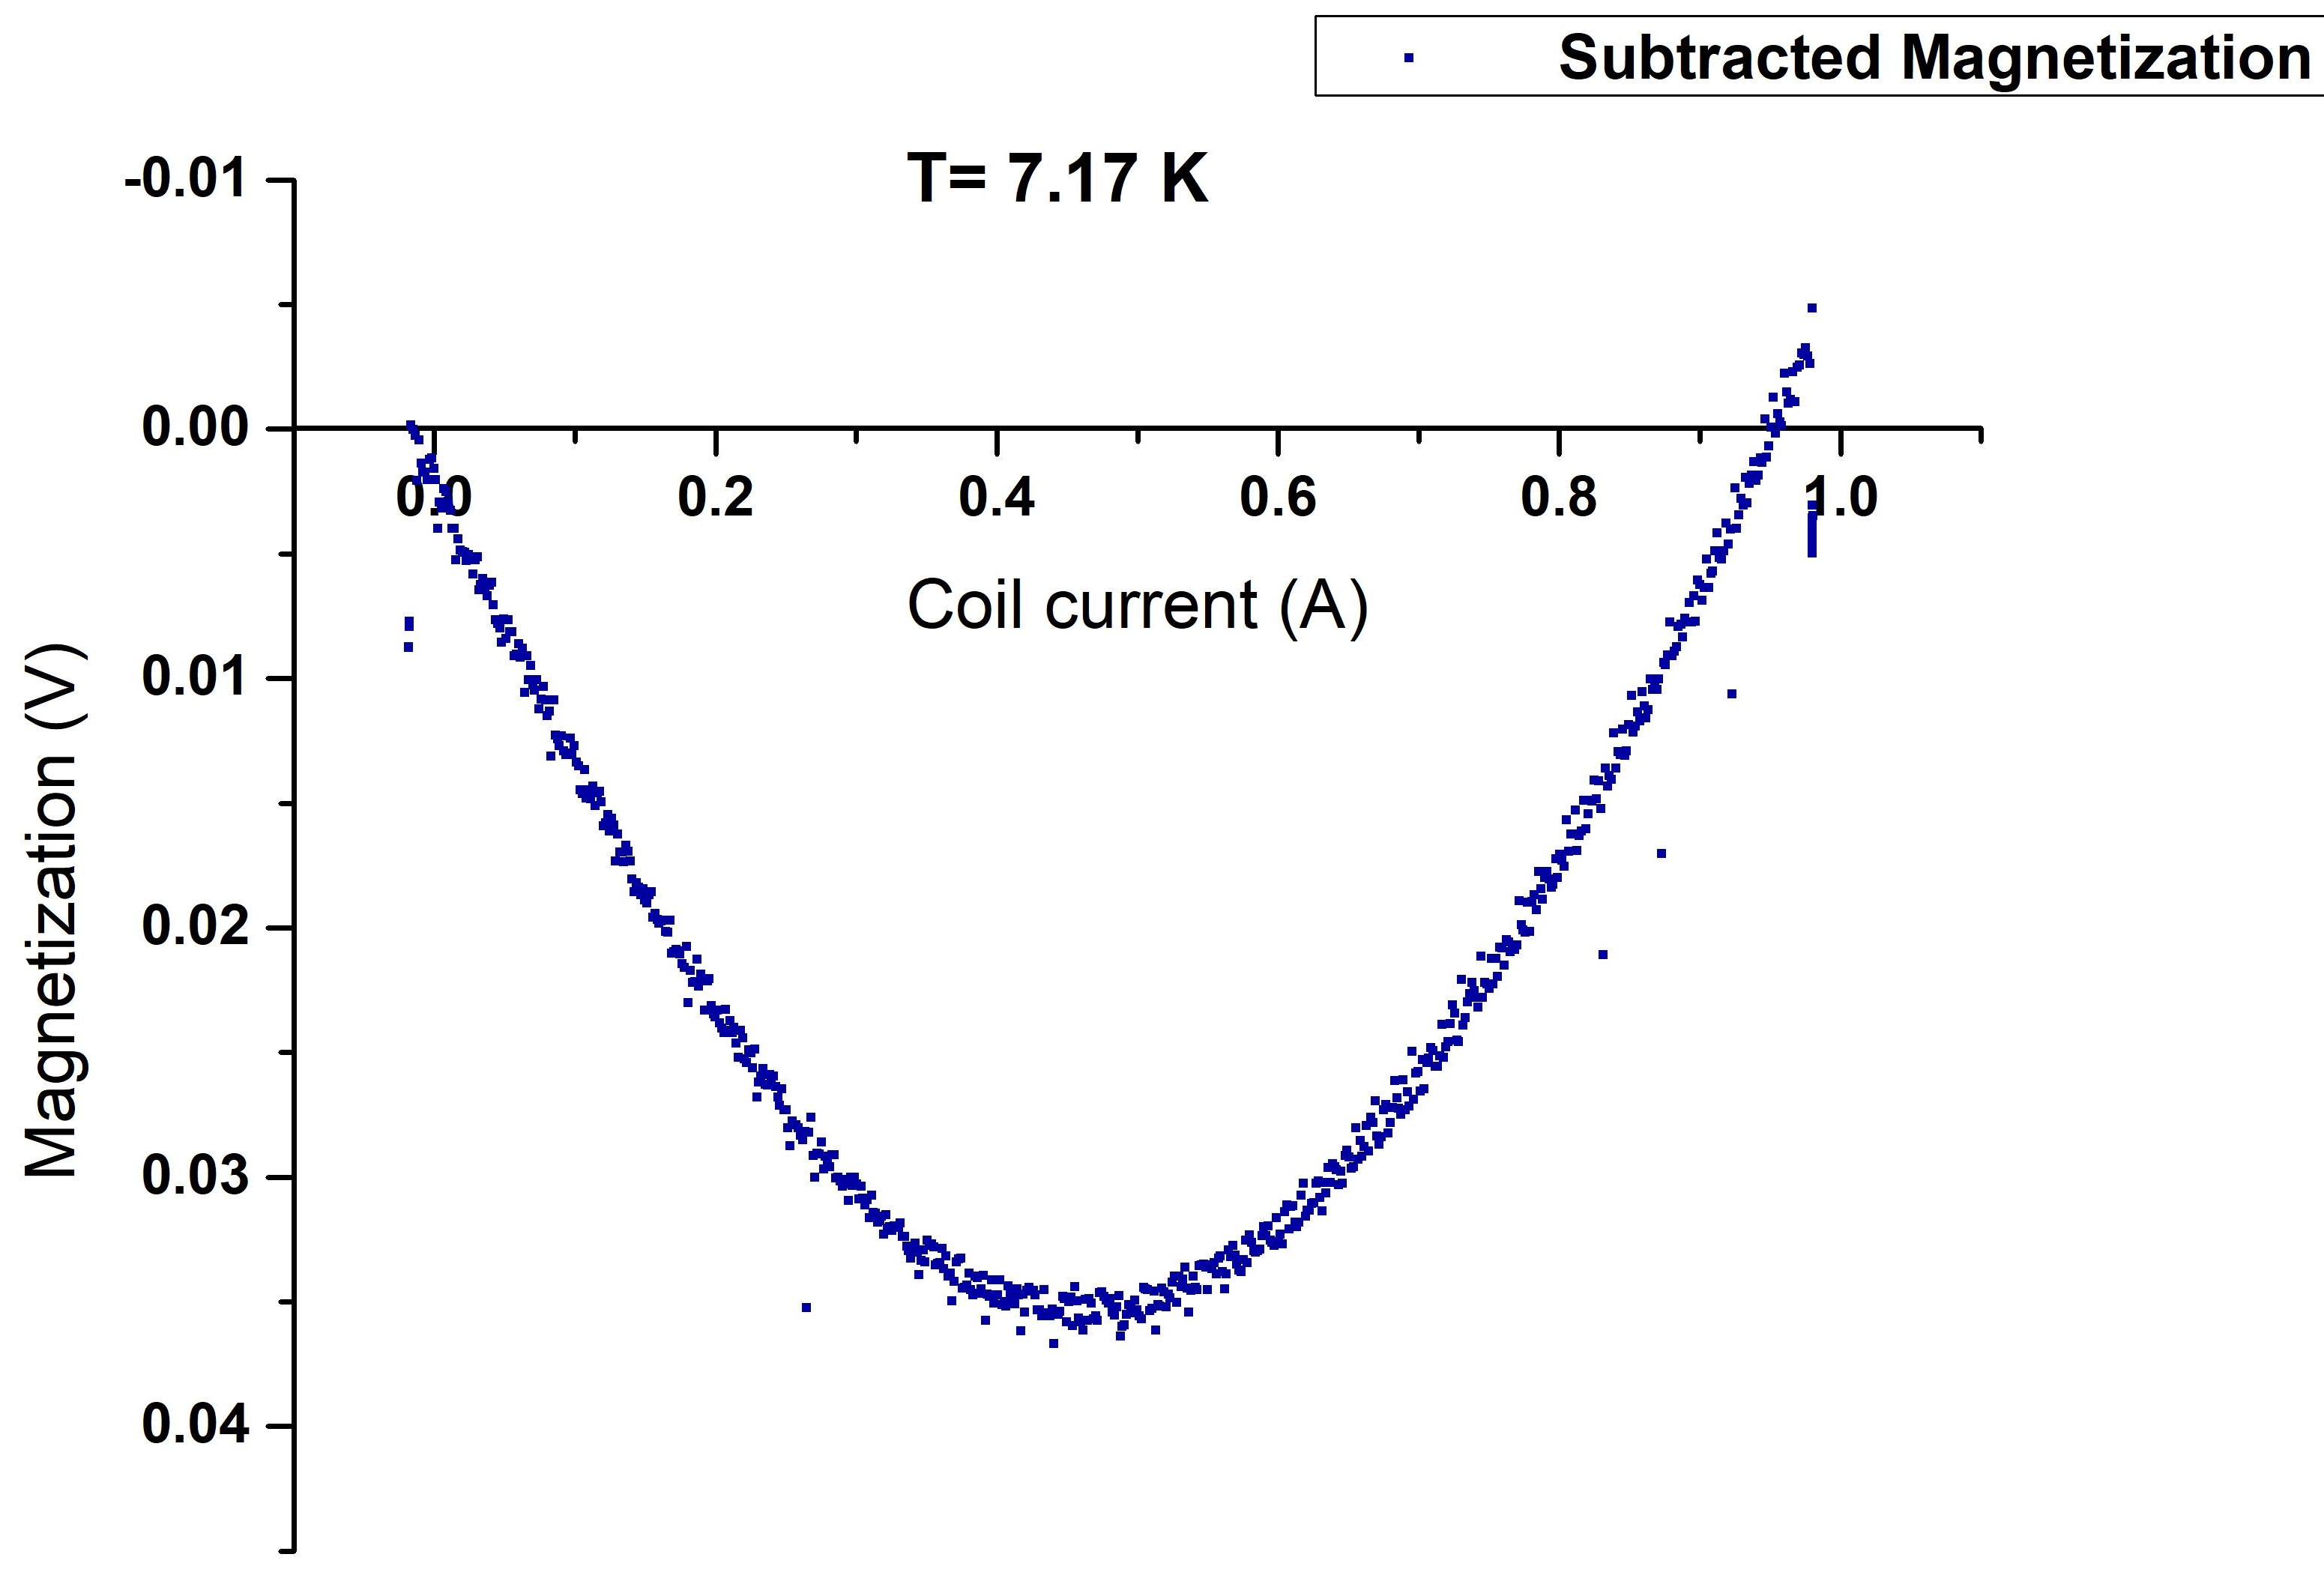
\includegraphics[scale=0.15]{717.jpg} 
\end{center}
\end{figure}

Bellow, the $H_{C}$ values were plotted against temperature and fitted according to Eq \ref{HC}, where we extracted the critical temperature at $T_{c}=7.109 \pm 0.012 K$ and $H_{0}= 814.702\pm  4.4025
$G with adjusted $R^{2}=0.9998$, meaning that the calculation is quite accurate.




\begin{figure}[H]
\centering
\caption{fitting according to function$H_{C}=H_{0} [1- (\dfrac{T}{T_{C}})^{2}]$.}
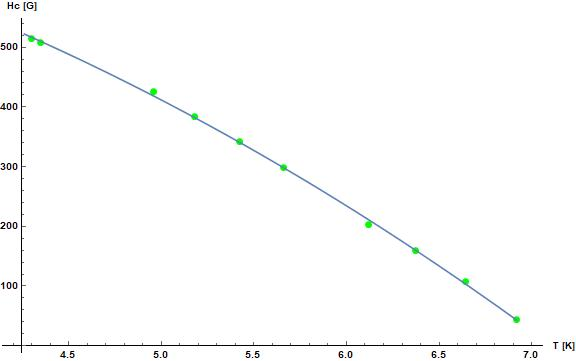
\includegraphics[scale=0.8]{HcT.jpg}
\end{figure}




A very pure sample of lead is a very characteristic example of Type I superconductors, specifically is the strongest type-I superconductor with critical temperature at $7.196$ K and critical field at $H_{C}=803$ G.\\

Further we extracted the demagnetizing factor for each temperature below $T_{C}$ and fitted the data according to Eq \ref{D}

\begin{figure}[H]
\centering
\caption{fitting according to function $D= 1- \dfrac{H_{max}}{H_{C}}$.}
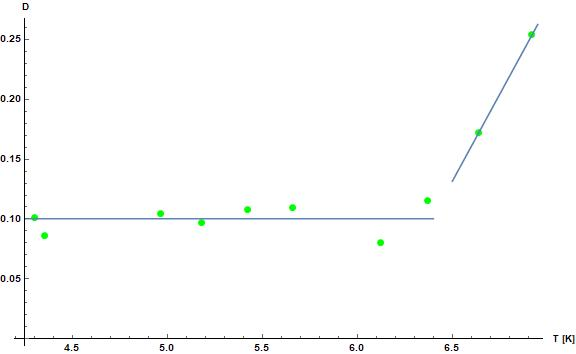
\includegraphics[scale=.8]{DT.jpg}
\end{figure}

D should be constant for the same sample against temperature, which is verified by our fit until we reach the vicinity of the critical temperature $T_{C}$, where we observe a linear increase therefore probably the loss of superconductivity. The value obtained for the steady slope is $D=0.099 \pm 0.004$, where considering that the demagnetizing factor for a cyllinder is $0$ and taking into account the factor of a probable field misalignment with the sample, we could guess that our sample's symmetry could be quite close to that.\\

The area contained in the $M-H$ plots corresponds to free Gibbs energy contributed by $M$, where the field H according to the coil current is given by
\begin{equation}
H=k I  \text { with } k=739 \mathrm{G} / \mathrm{A}
\end{equation}







\begin{figure}[H]
\begin{center}
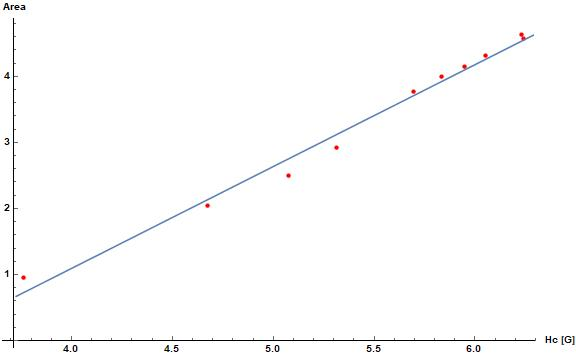
\includegraphics[scale=.6]{doublog.jpg}
\caption{double logarithmic plot fitted linearly.}
\end{center}
\end{figure}


We obtained $Log(Area)= 5.076 + 1.542 Log(H_{C})$, giving a slope at $1.542 \pm 0.393$, with adjusted $R^{2}=0.983$.

According to Eq \ref{freeE}, the area should be proportional to $H_{C}^{2}$, where considering a double logarithmic plot we obtain 

\begin{equation}
\frac{\log \left(A_{2} / A_{1}\right)}{\log \left(H_{C 2} / H_{C 1}\right)}=\frac{\log \left(H_{C 2}^{2} / H_{C 1}^{2}\right)}{\log \left(H_{C 2} / H_{C 1}\right)}=2
\end{equation}





\section{Flux change curves characterized by field
strength }
In this part of the experiment we obtained the Magnetization curves against resistance and then we plotted the flux change at the phase transition as a function of the corresponding field
strength (warming up and cooling down M(T) curves), subtracting again the constant this time background at the highest temperatures of the magnetization, as illustrated bellow. In the lab, we sweept the current values in order to increase the current in the sample heater over $T_{c}$ and then the same curves were obtained for cooling the sample heater by sweeping backwards in the same rate.\\

 
The black points in the plots represent the heating of the sample and the red points represent the cooling down, with the field constant. \

Further we determined the Meissner-Ochsenfeld effect in fraction by dividing the maximum value for heating with the one for cooling, concerning to the same field strength, against the current.




\begin{figure}[H]
\begin{center}
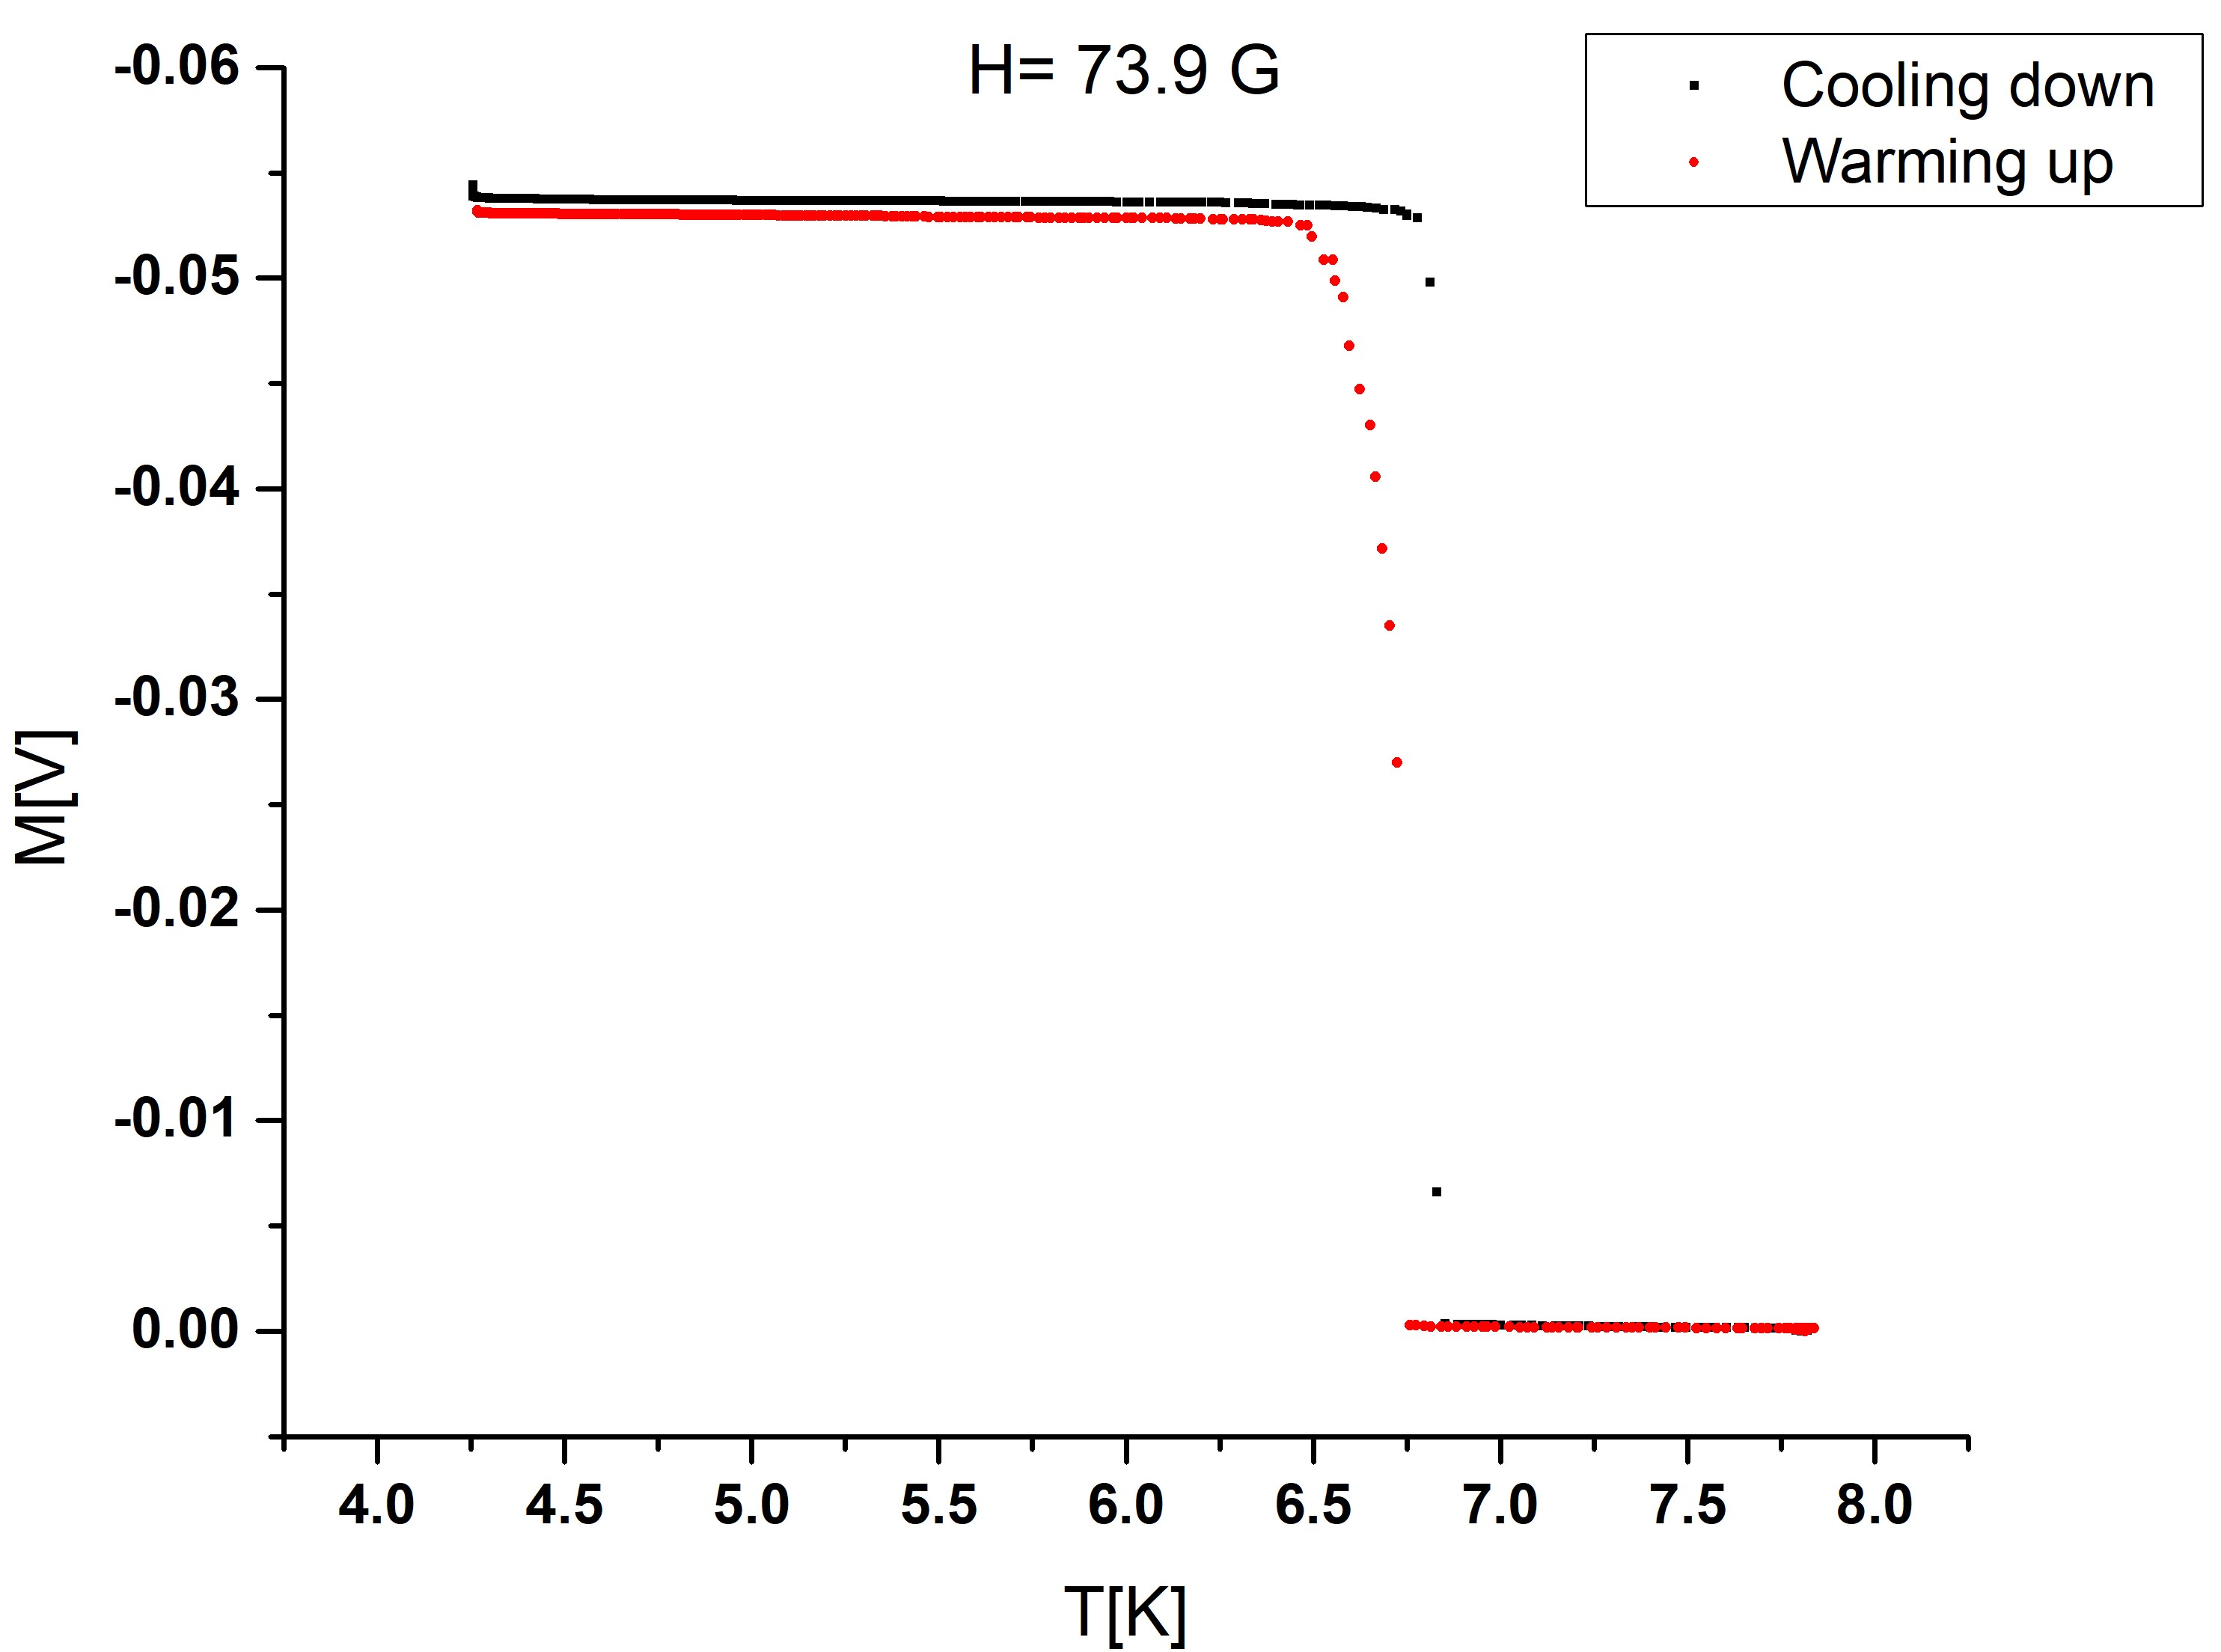
\includegraphics[scale=0.35]{finalone.jpg}
\end{center}
\end{figure}




\begin{figure}[H]
\begin{center}
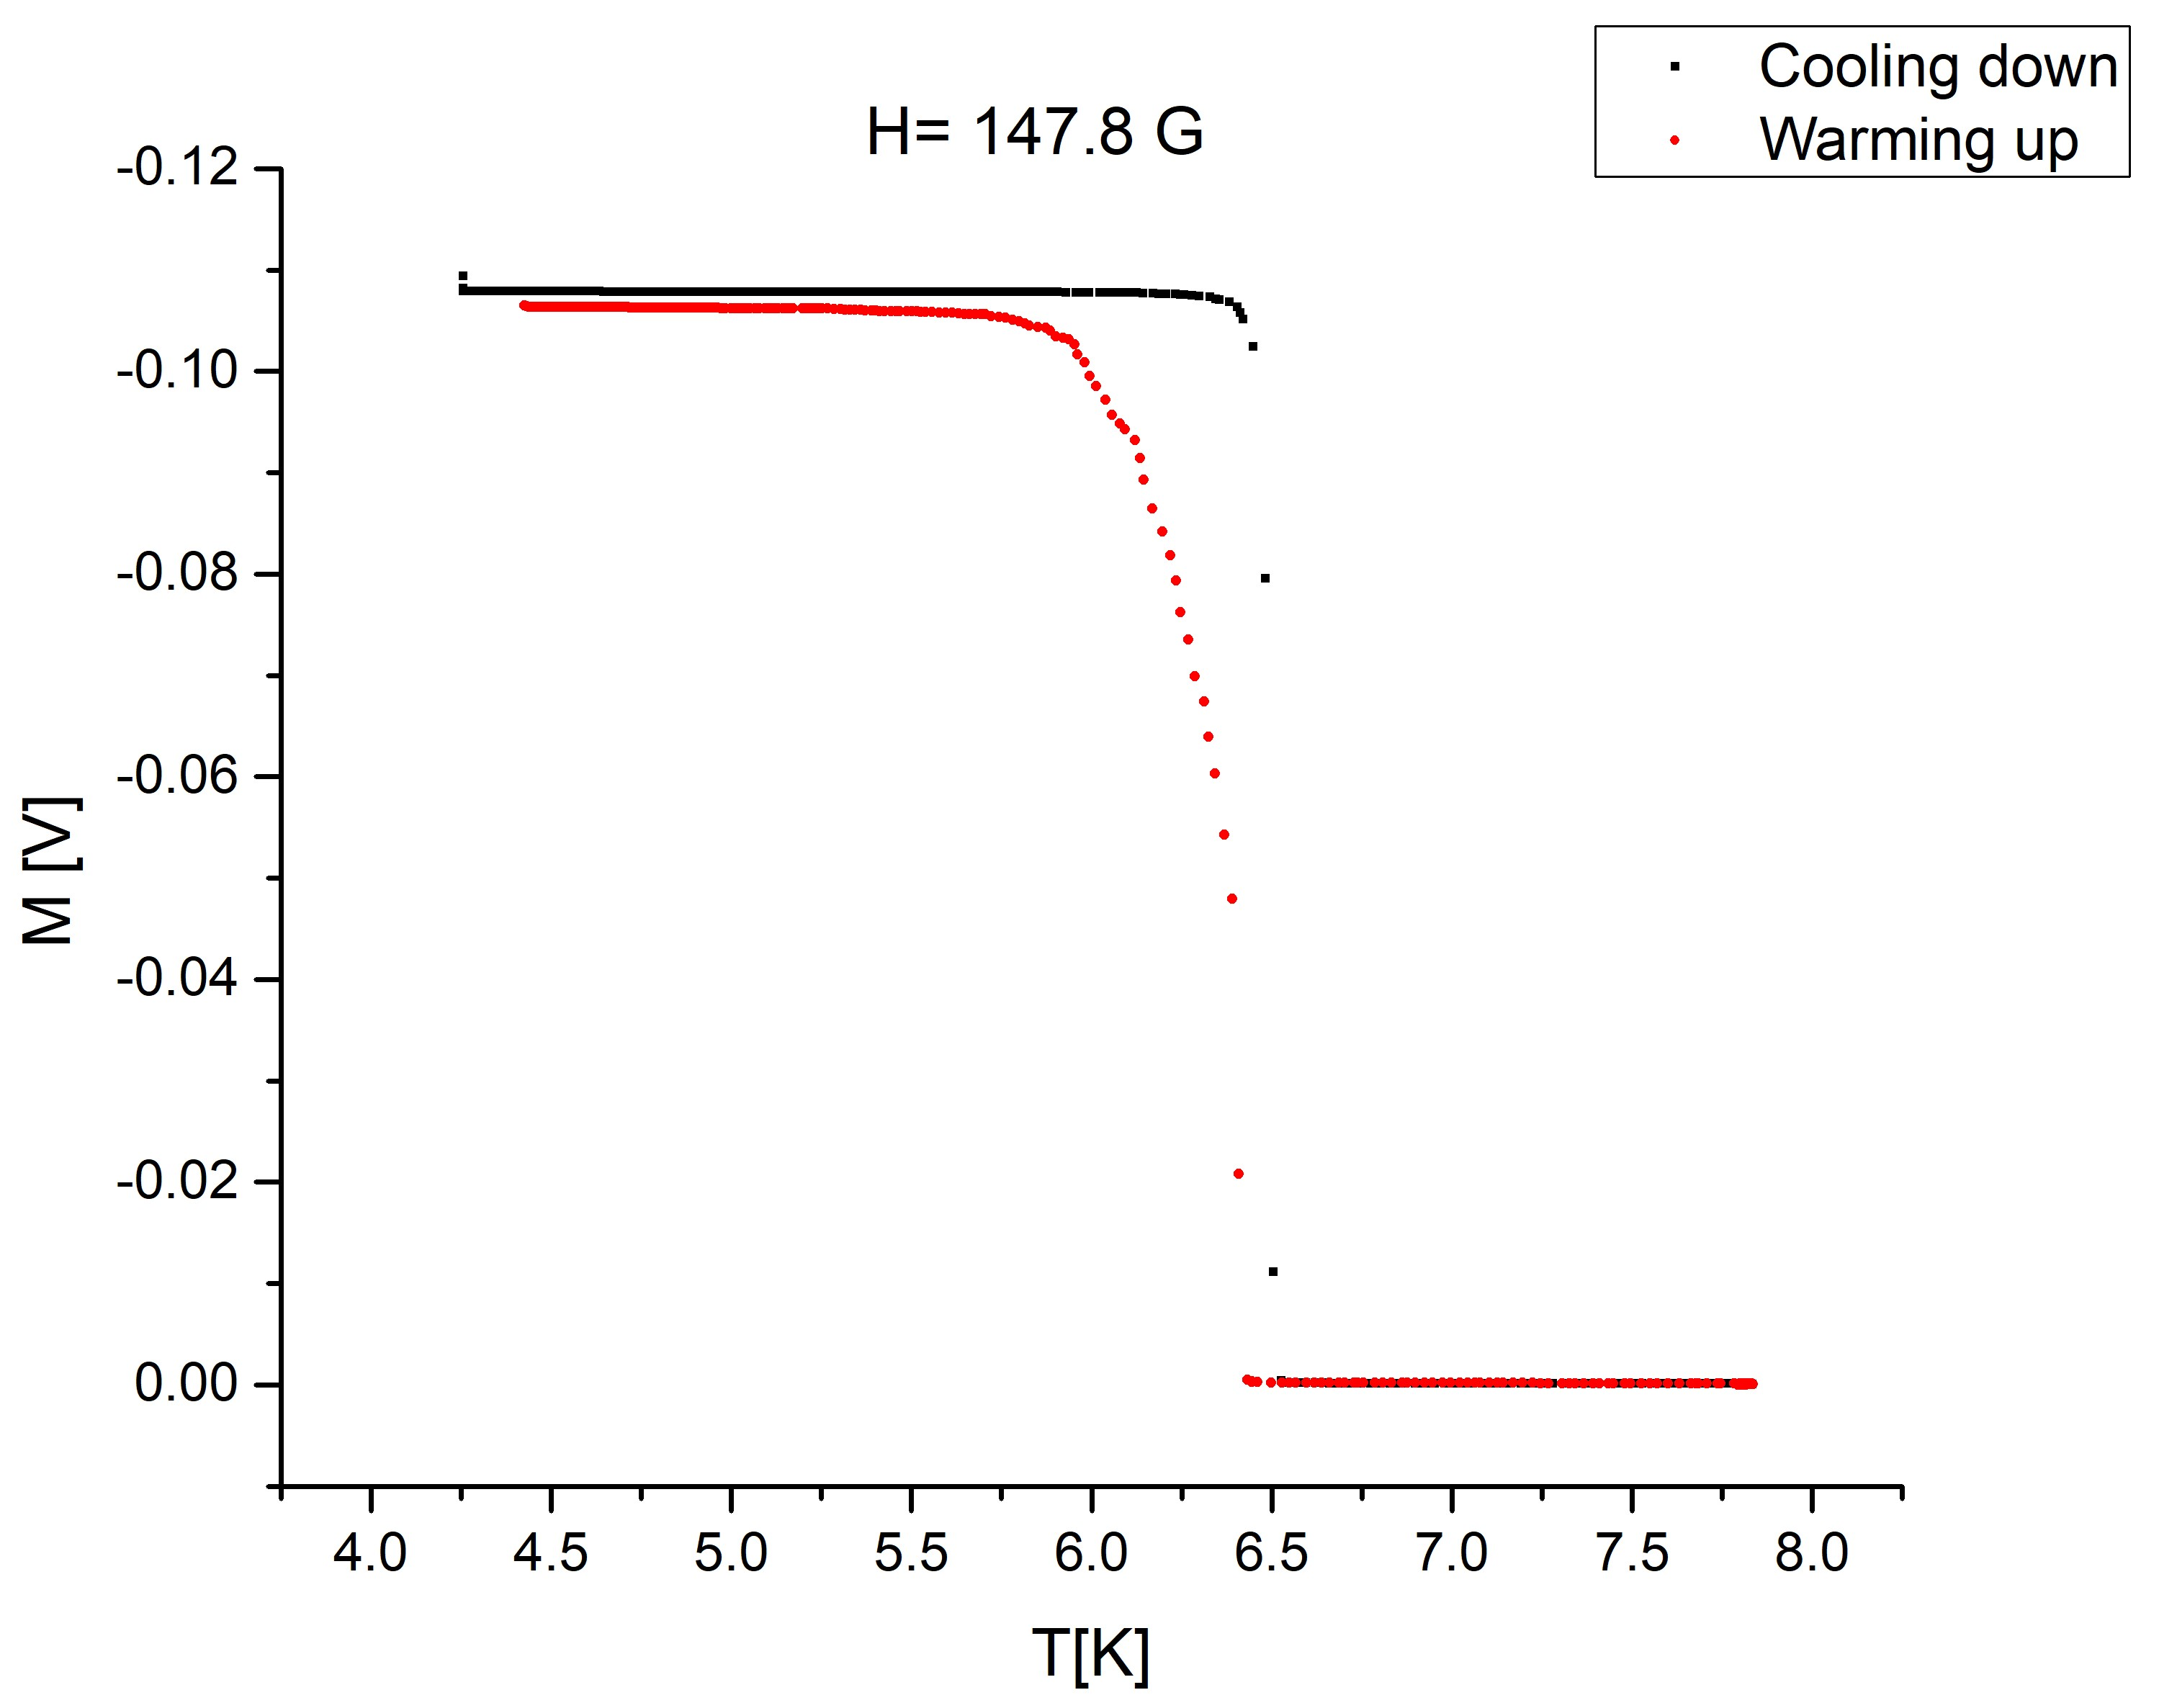
\includegraphics[scale=0.35]{finaltwo.jpg}
\end{center}
\end{figure}



\begin{figure}[H]
\begin{center}
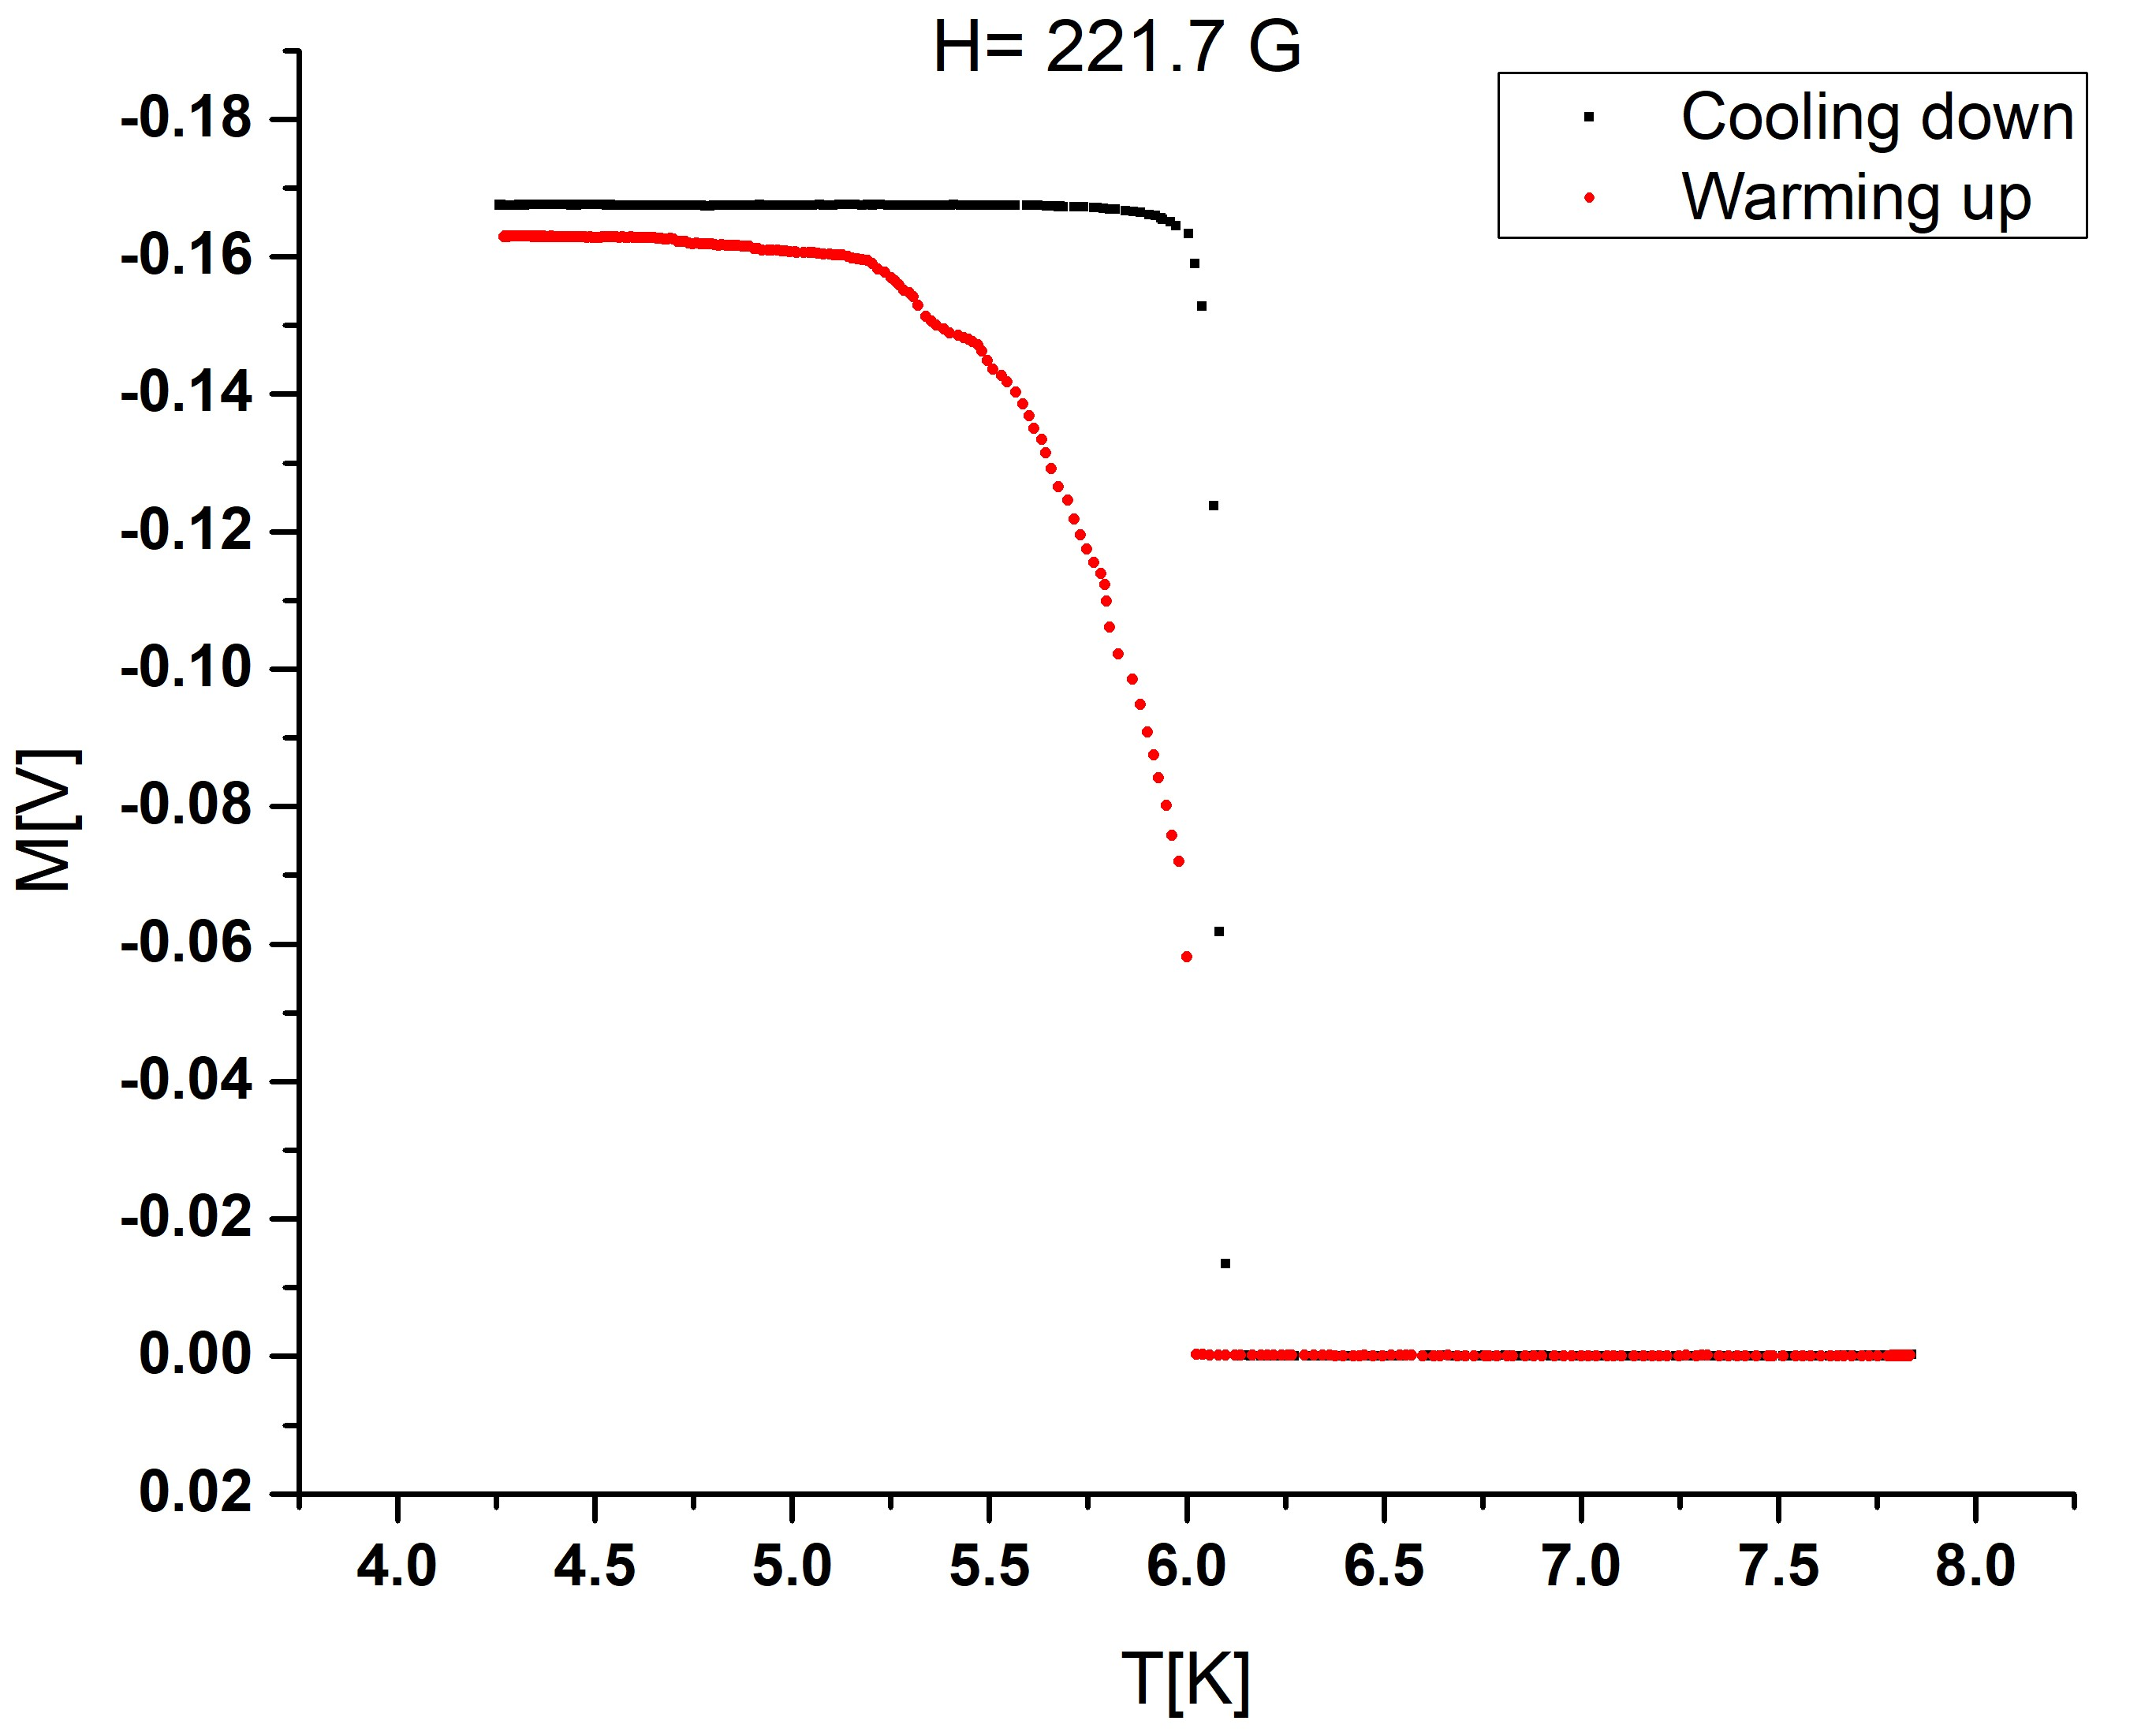
\includegraphics[scale=0.35]{finalthree.jpg}
\end{center}
\end{figure}


\begin{figure}[H]
\begin{center}
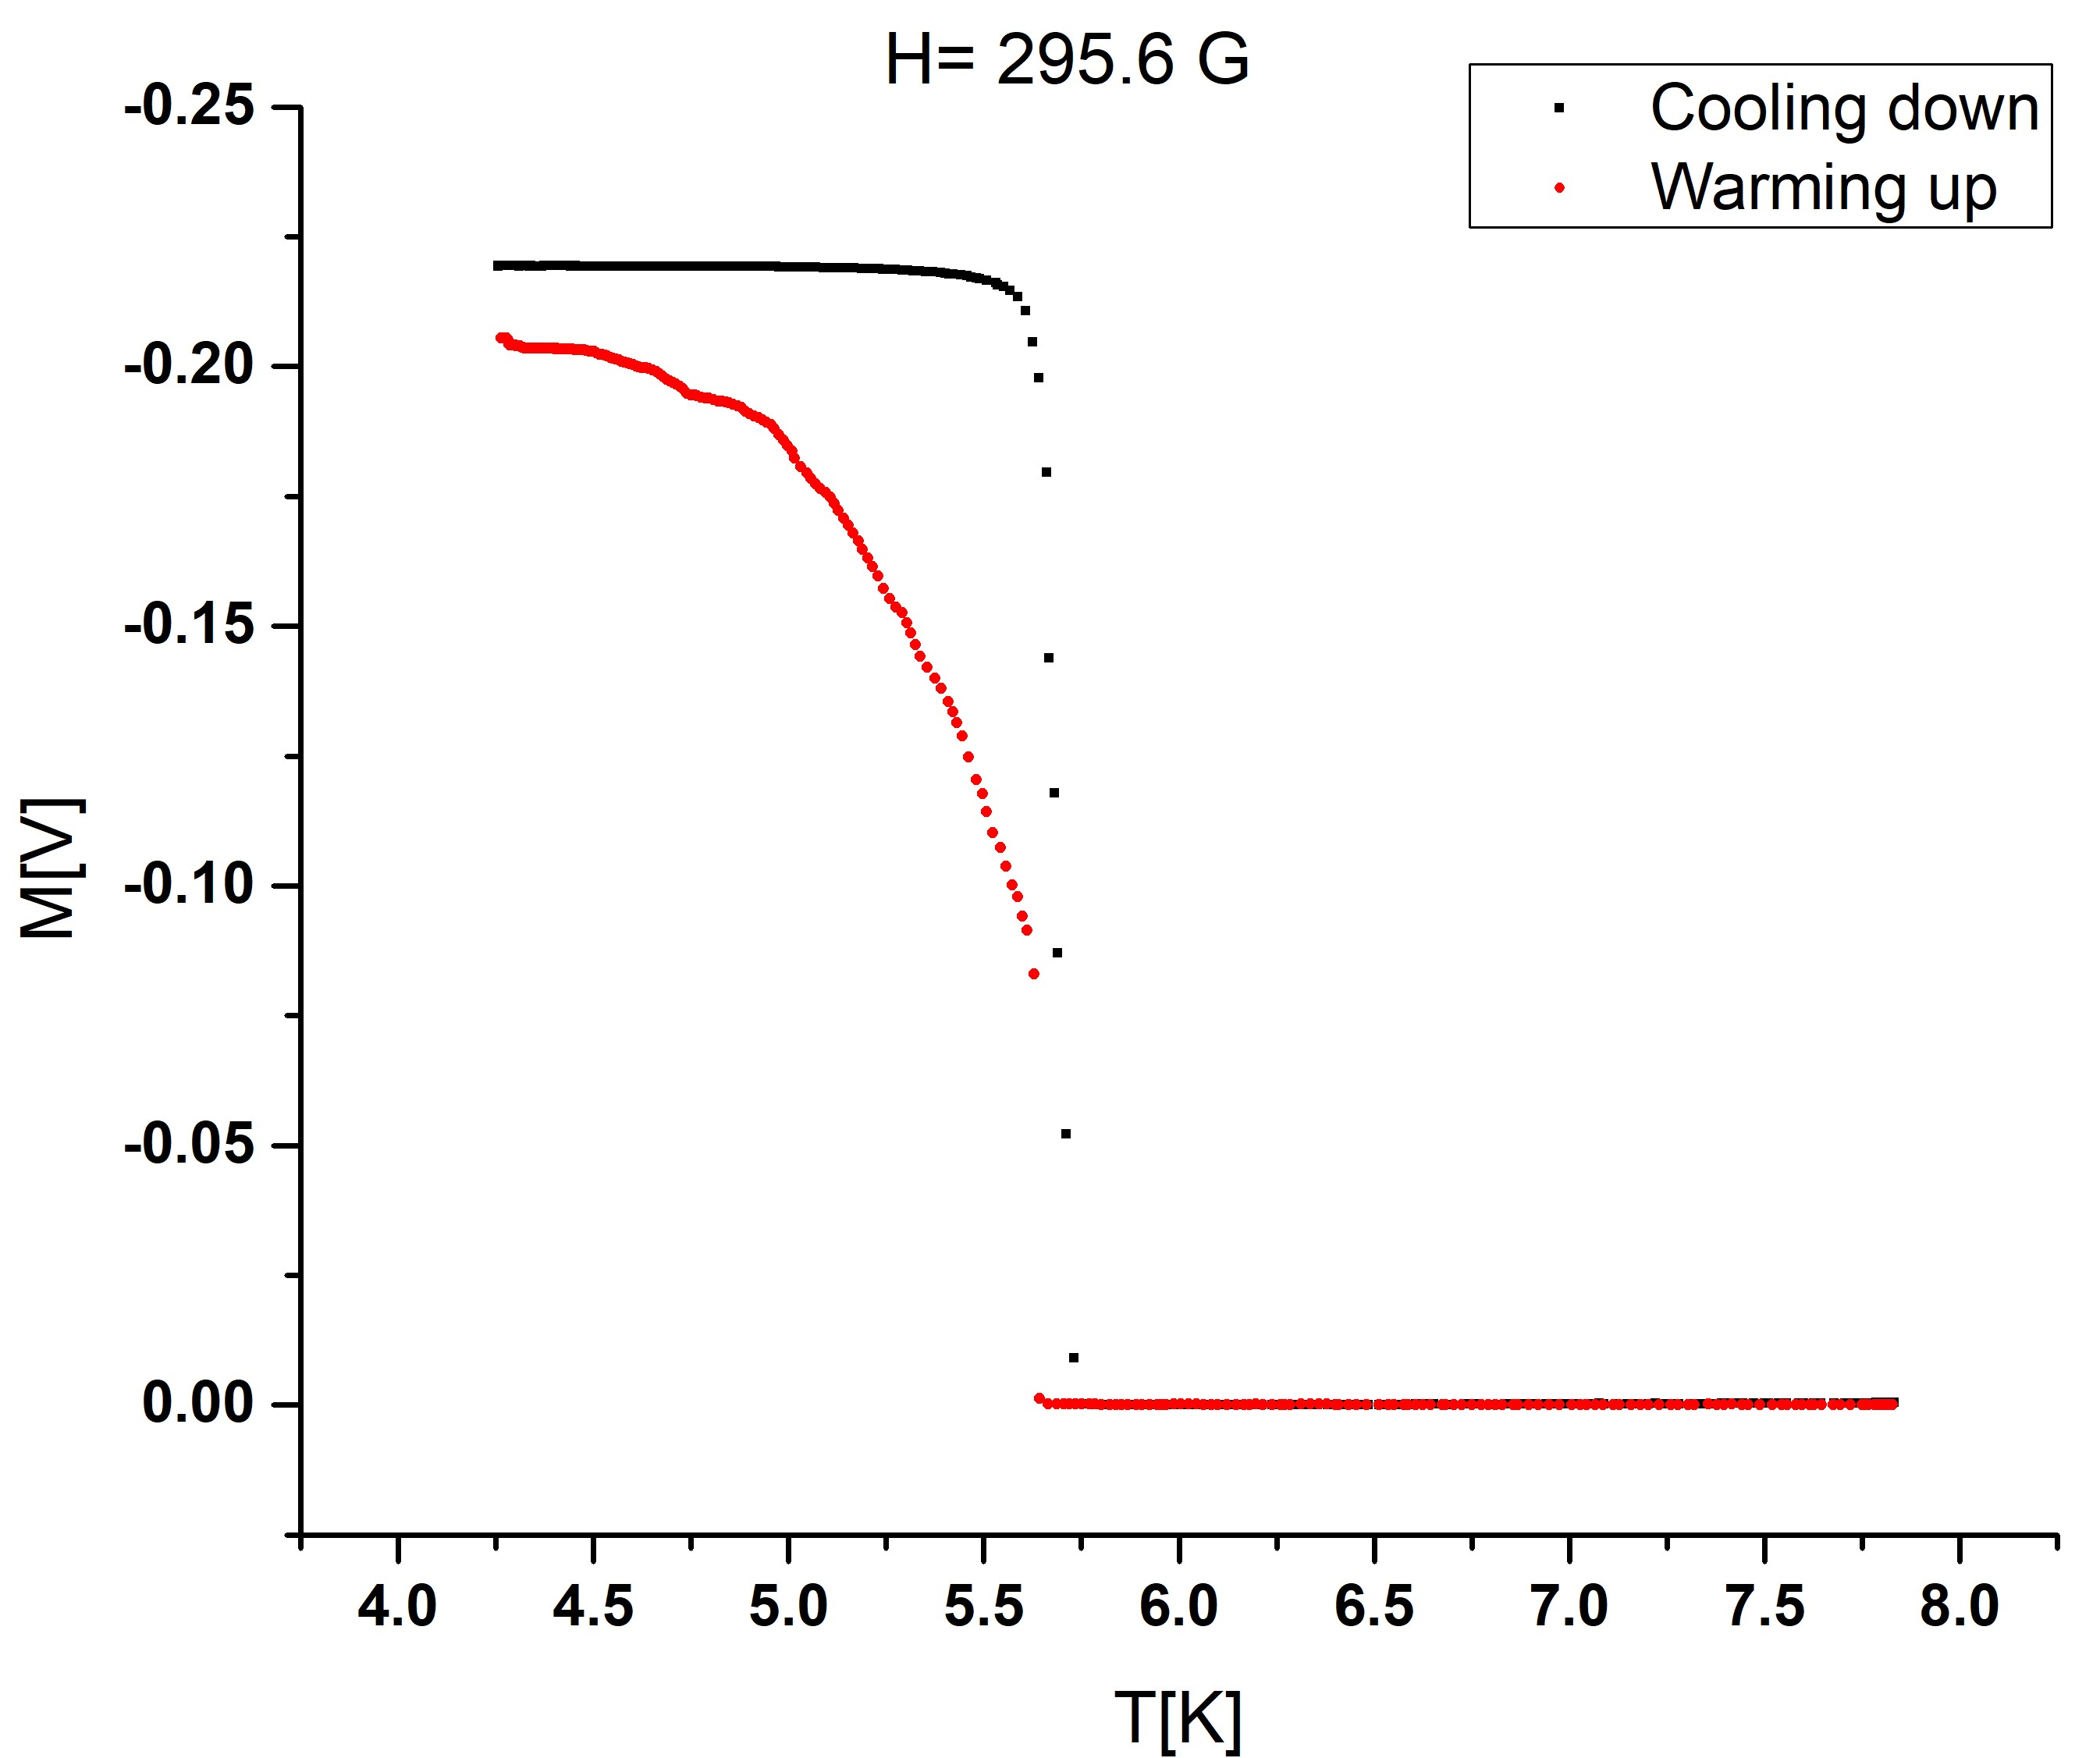
\includegraphics[scale=0.35]{finalfour.jpg}
\end{center}
\end{figure}

\begin{figure}[H]
\begin{center}
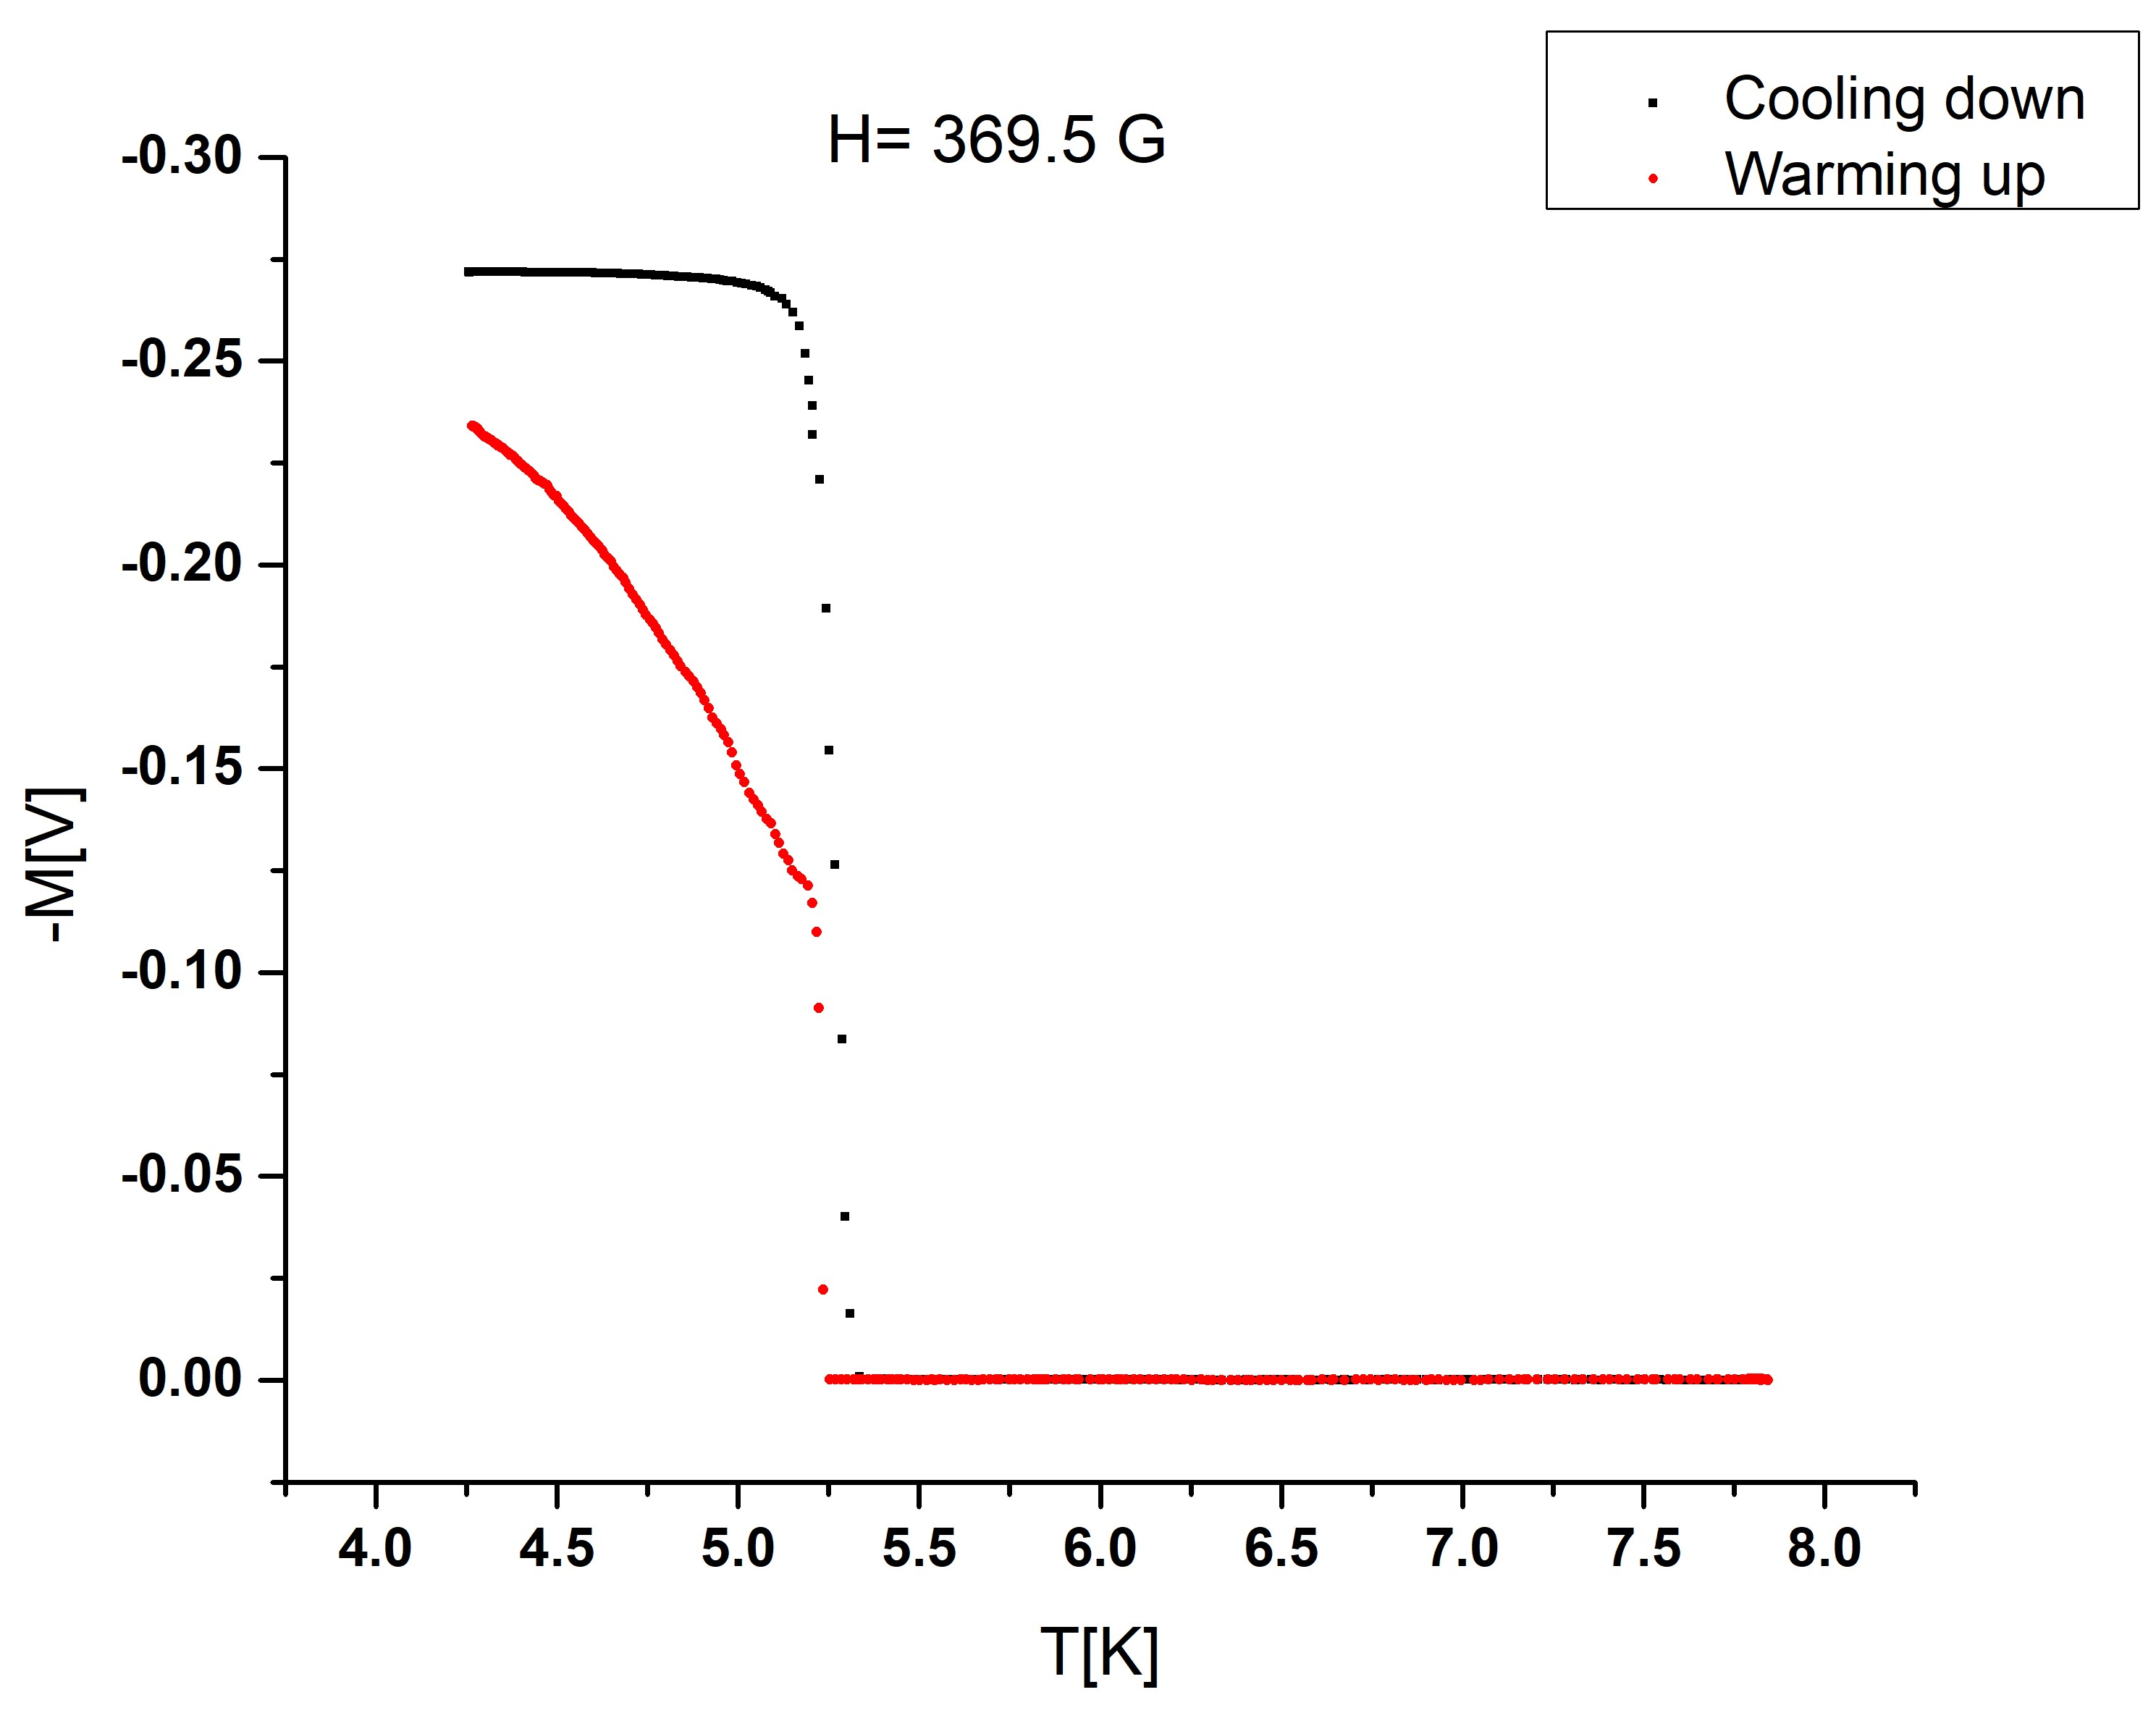
\includegraphics[scale=0.35]{finalfive.jpg} 
\end{center}
\end{figure}


\begin{figure}[H]
\begin{center}
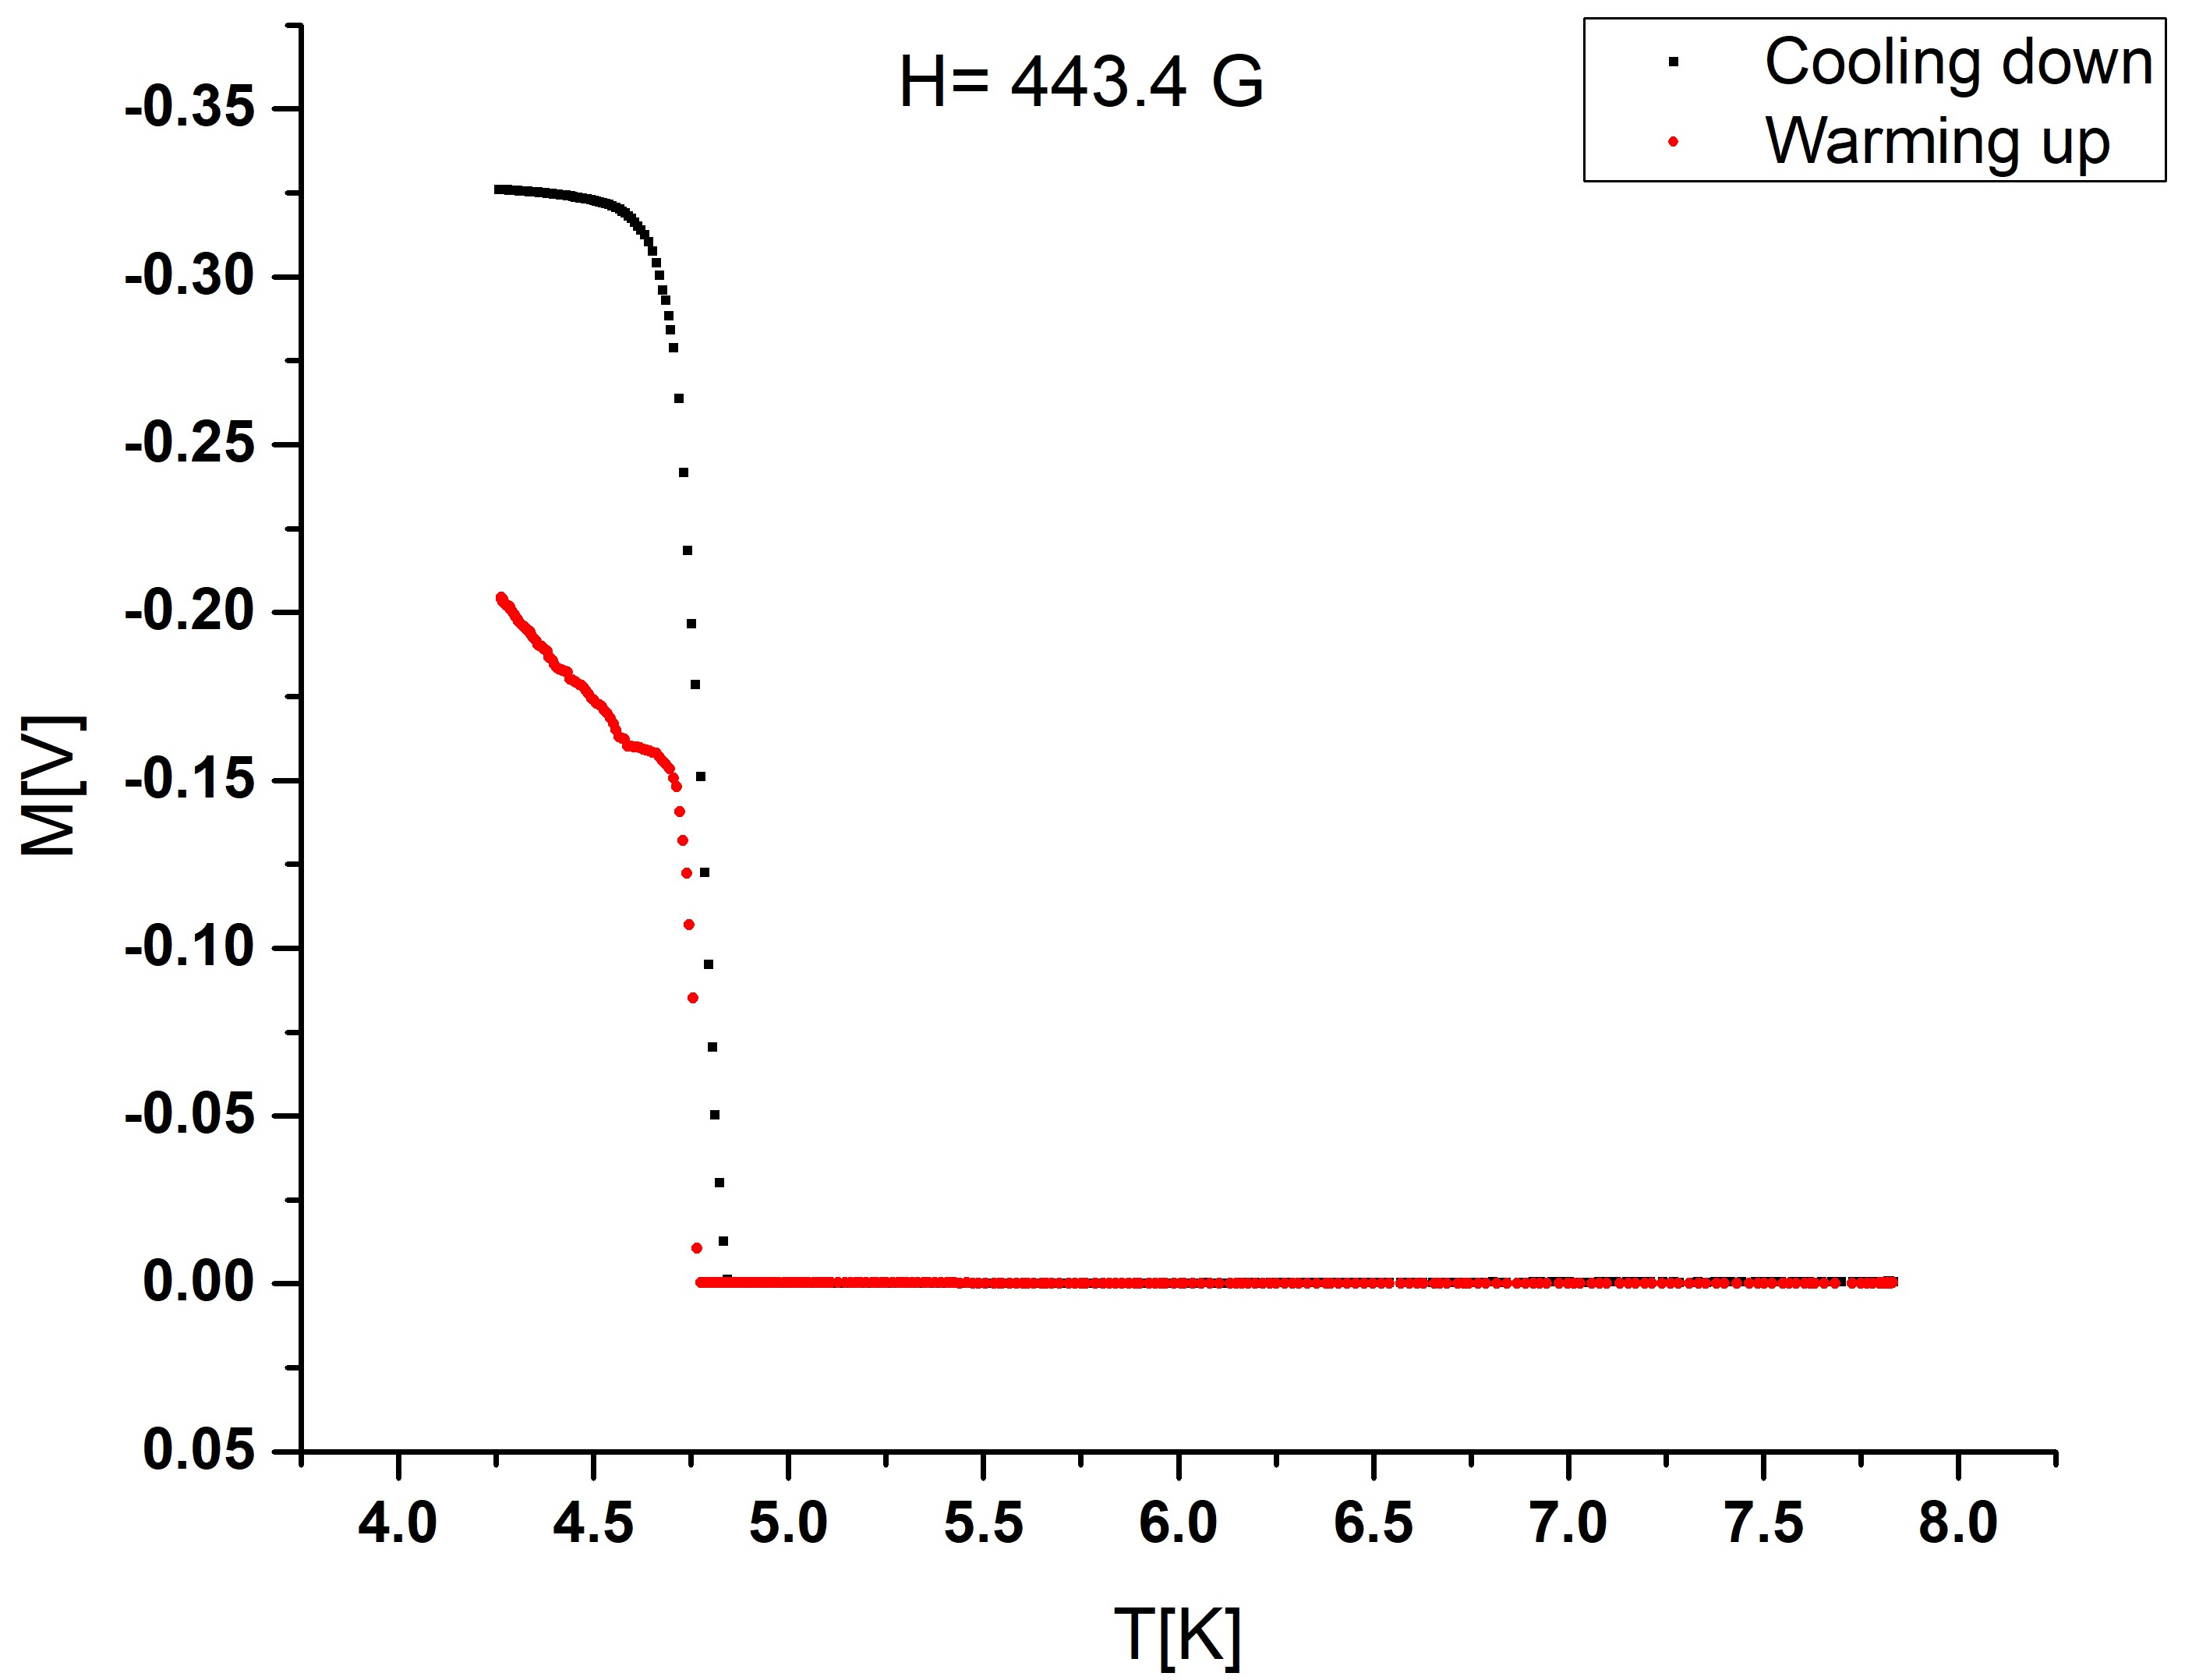
\includegraphics[scale=0.35]{finalsix.jpg}
\end{center}
\end{figure}


\begin{figure}[H]
\begin{center}
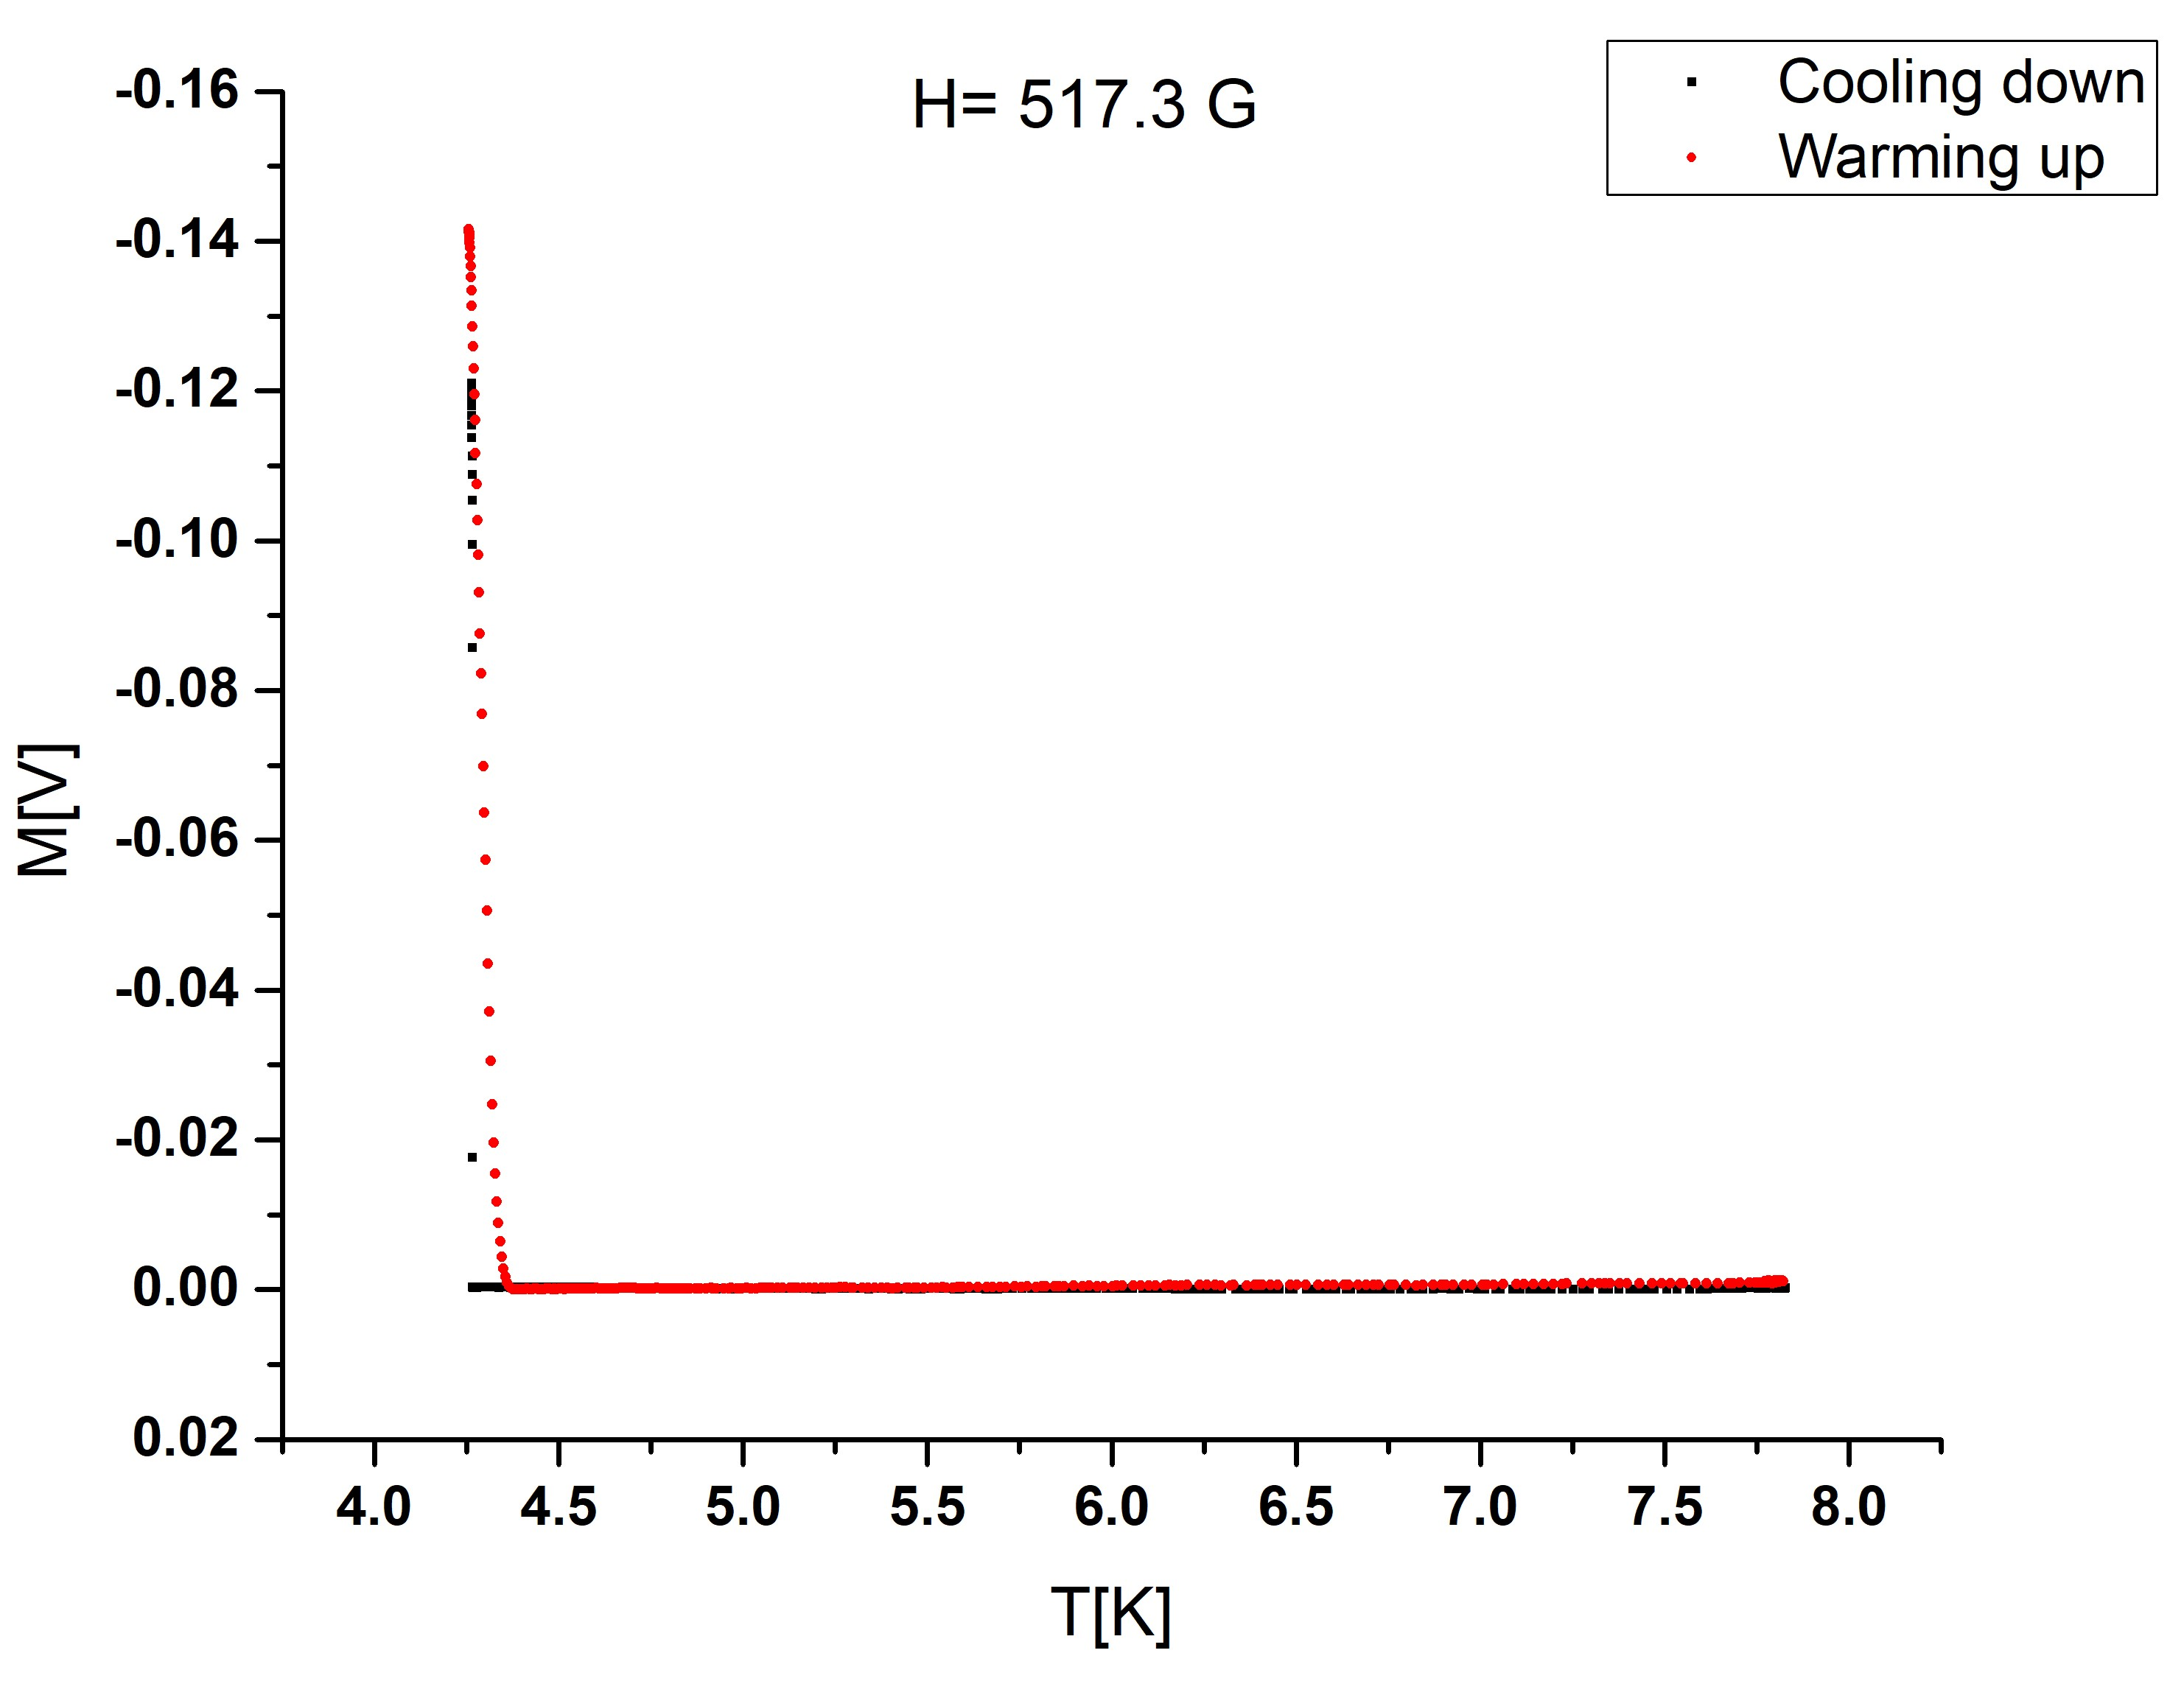
\includegraphics[scale=0.35]{finalseven.jpg}
\end{center}
\end{figure}





\begin{figure}[H]
\begin{center}
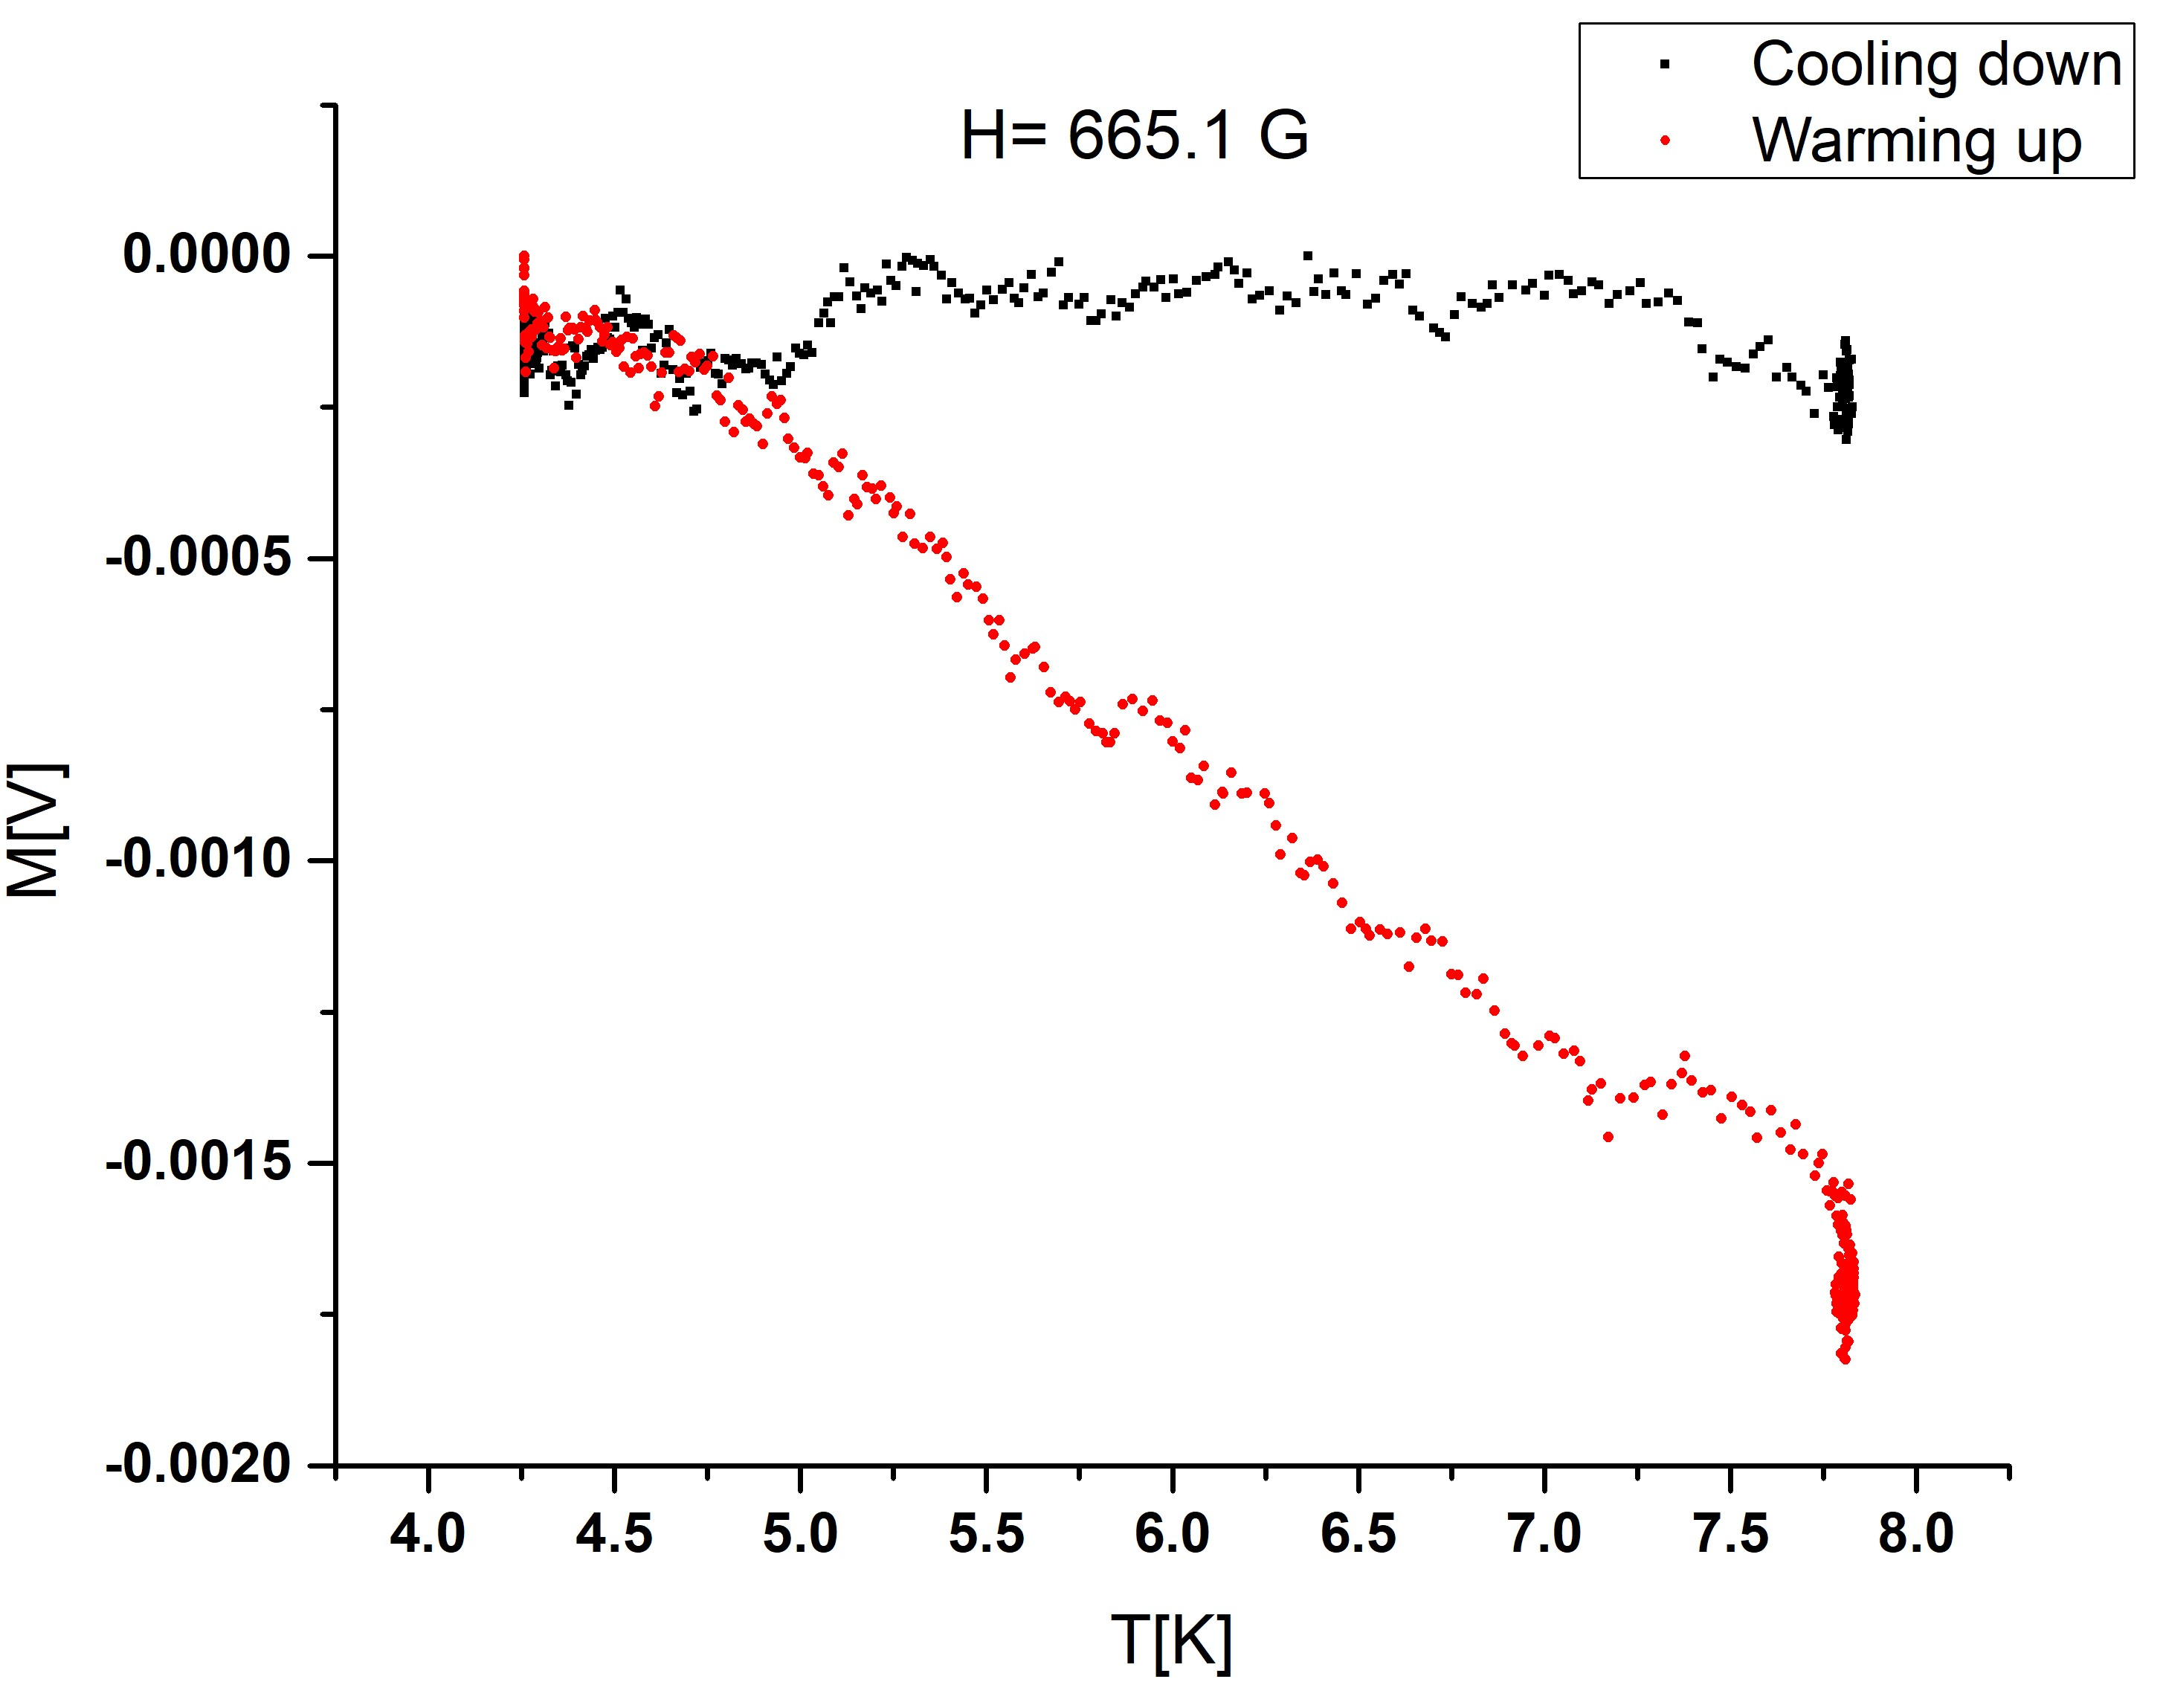
\includegraphics[scale=0.35]{finaleight.jpg}
\caption{Magnetization as a function of applied field}
\end{center}
\end{figure}



We observe from the plots above that the critical temperature is decreasing with the increase of the field strength, thus the Meissner-Ochsenfeld fraction will decrease too, as illustrated in Fig \ref{moe}.



\begin{figure}[H]
\centering
\caption{Meissner-Ochsenfeld fraction}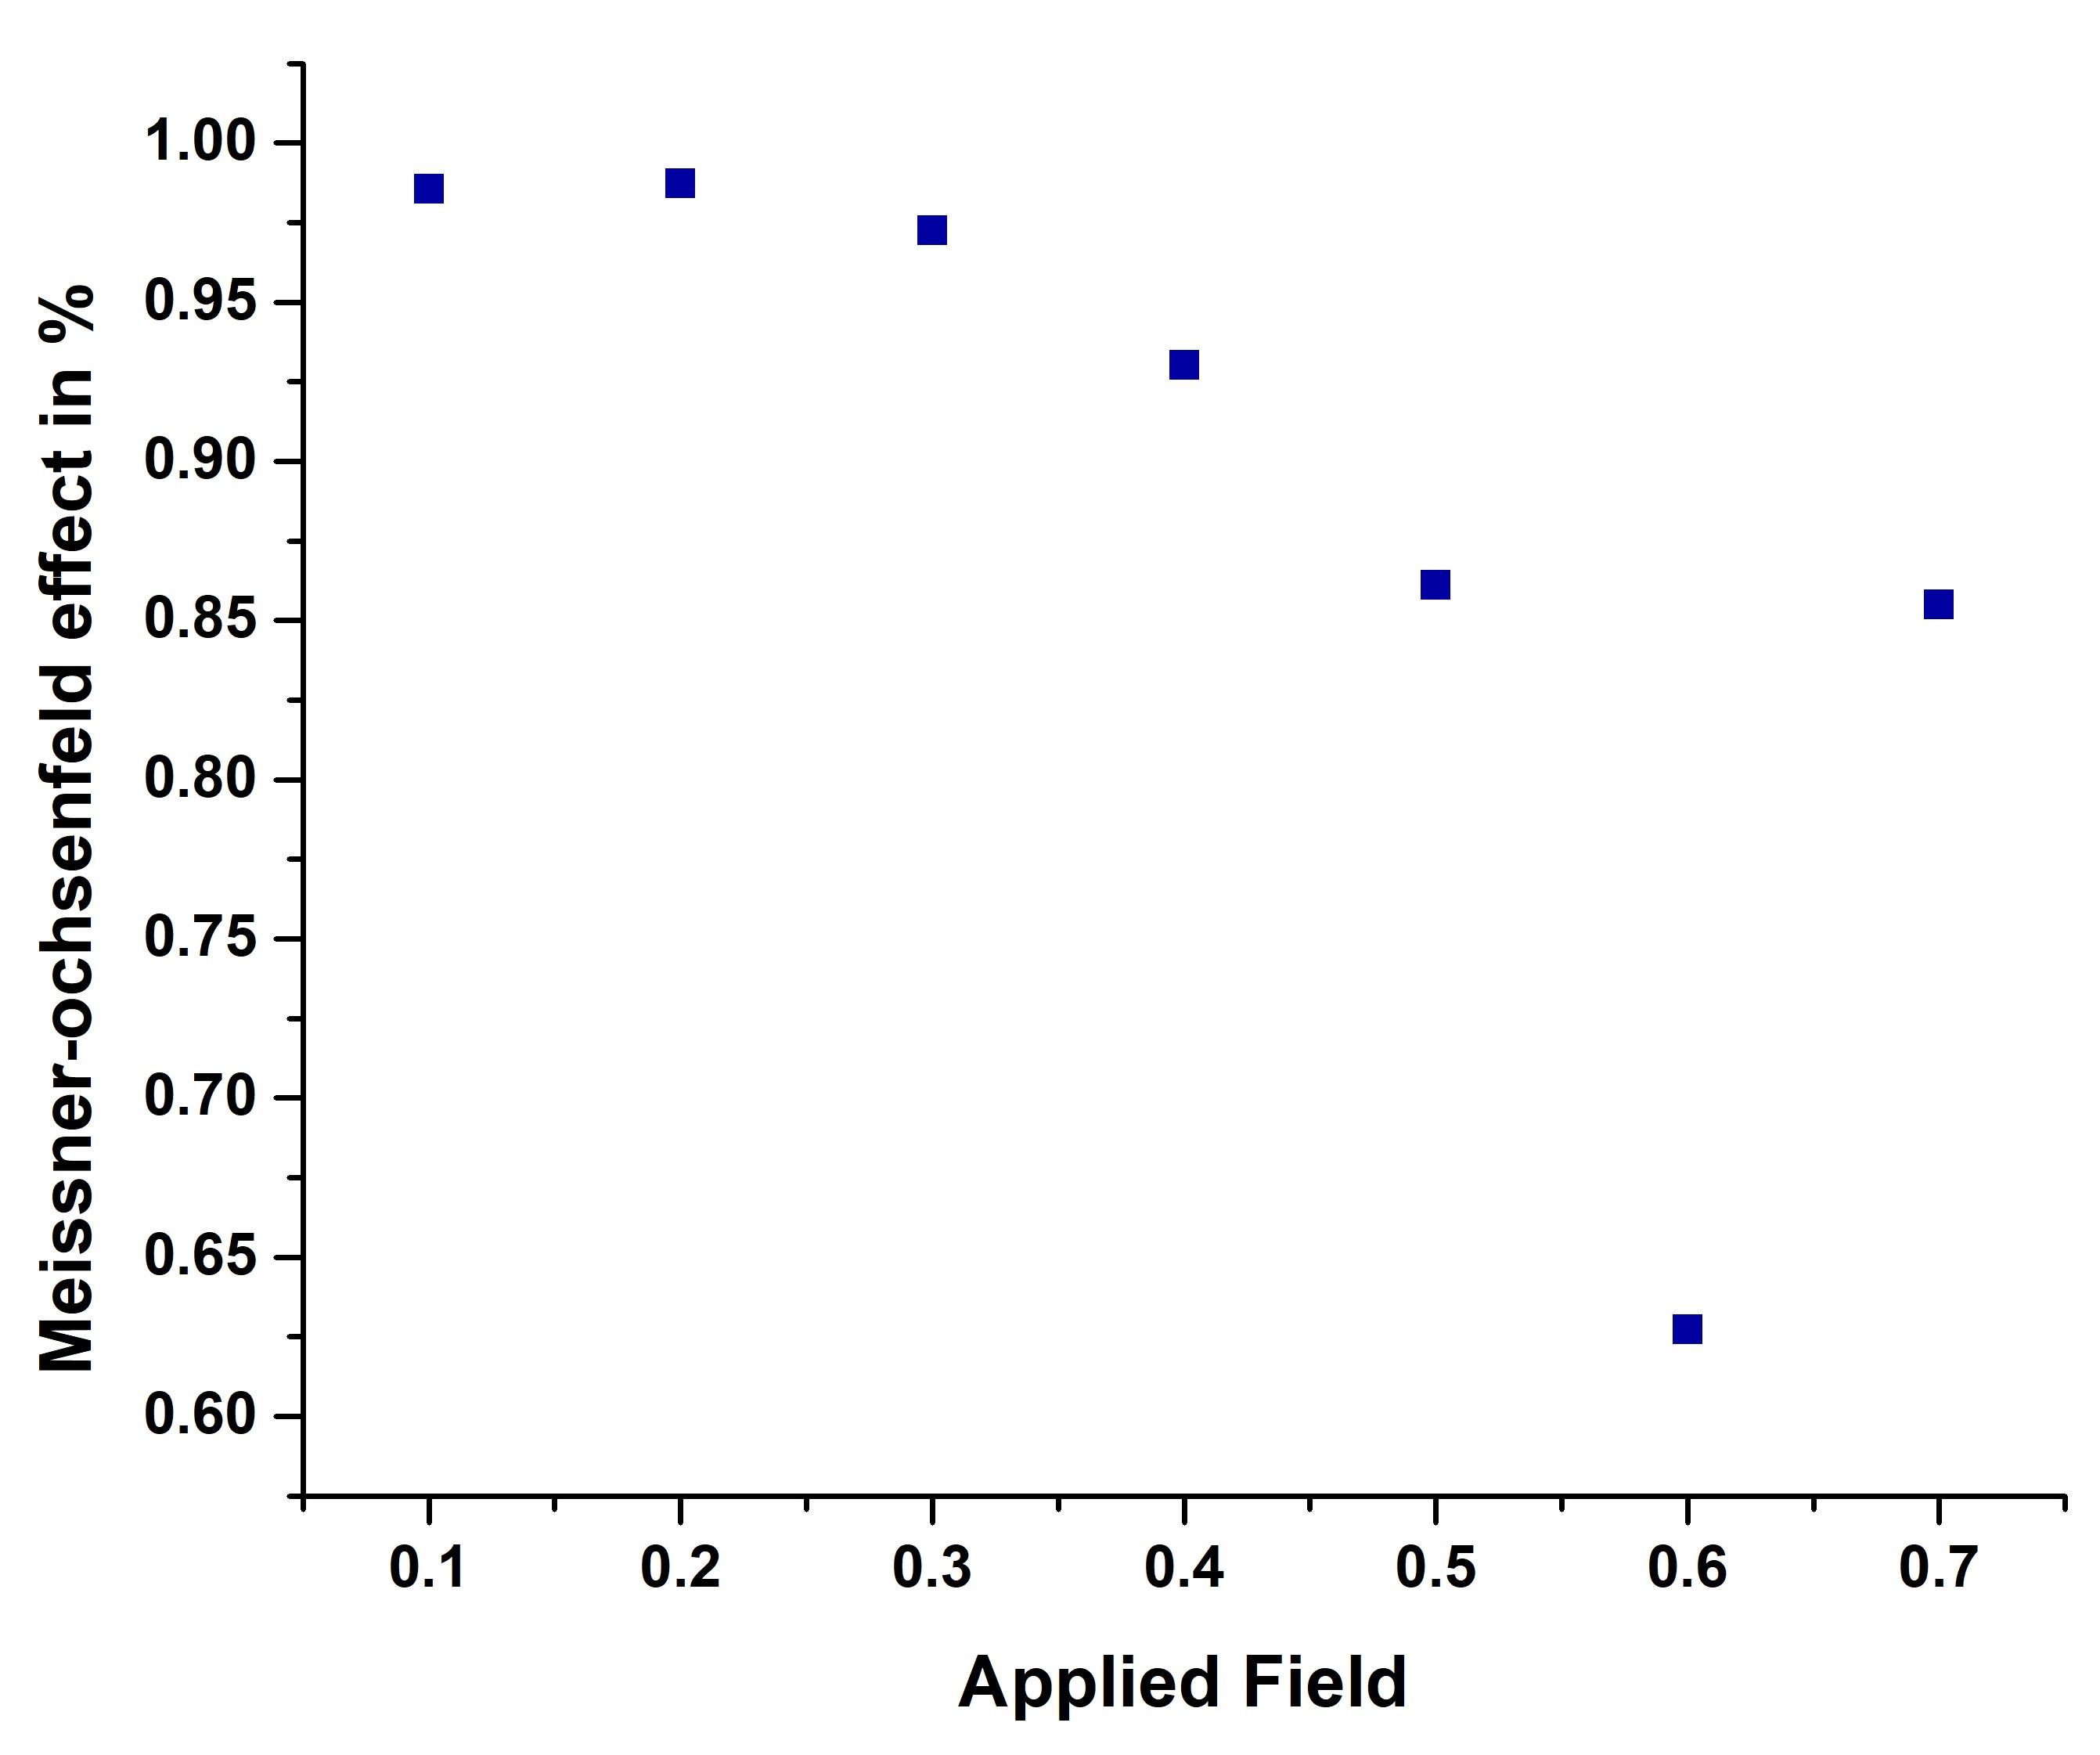
\includegraphics[scale=0.5]
{moe.jpg}  
\label{moe}
\end{figure}

The plot obeys the normal decreasing behaviour and its maximum value does not exceed 1. The last point corresponding to $0.7 A$ is the vinicity that is higher than the critical temperature of Lead so the superconductivity is lost.


\begin{thebibliography}{99}



\bibitem{kittel} 
Kittel, Charles, Introduction to Solid State Physics, 7th Ed., Wiley, (1996)


\bibitem{script} Script of the Practical course M,
Experiment M2.4:
Magnetization of a superconductor, Version 2014-07-14, Universitat zu Koln
II. Physikalisches Institut 

\bibitem{1} \url{http://hyperphysics.phy-astr.gsu.edu/hbase/Solids/scond.html}

\bibitem{meis} \url{http://hyperphysics.phy-astr.gsu.edu/hbase/Solids/meis.html#c1}


\bibitem{tinkham}\url{http://copilot.caltech.edu/documents/395-tinkham_intro_superconductivity_2nded_ch1_ch2.pdf}


\bibitem{demag} \url{http://www.phys.ubbcluj.ro/~iosif.deac/courses/ASSP/7_superconductivity.pdf}

\bibitem{slides}  \url{https://www.slideshare.net/VighneshDamodar/magnetic-properties-and-superconductivity}

\bibitem{Dfact} \url{http://ezphysics.nchu.edu.tw/15_course/sc_kuo/SC\%20ch6\%20&\%20ch7.pdf}

\bibitem{intermediate}
Vladimir Kozhevnikov, Intermediate State in Type-I Superconductors\\
 \url{https://www.intechopen.com/books/superfluids-and-superconductors/intermediate-state-in-type-i-superconductors}




\end{thebibliography}




\end{document}
